% March 2015 (TOC contents linked in red in pdf file)
%This template was prepared by Dorothea F. Brosius of the 
%Institute for Electronics and Applied Physics, University of Maryland, College Park, MD
%The template was last updated in March 2015
%Thesis Main Page used with thesis.sty based on the
%University of Maryland Electronic Thesis and Dissertation (ETD) Style Guide

%The YourInformation file was created by Freja Nordsiek, 2014.
%Code for linking the TOC titles to the text in the pdf file was created by Freja Nordsiek, 2014.


% Select the version that fits how you are making this LaTeX document (its driver).
% The first two are the most likely ones to be needed.
%
\newcommand{\mydriver}{pdftex} %Making a PDF directly using pdflatex.
%\newcommand{\mydriver}{dvipdfmx} %Making a DVI and converting that to PDF using dvipdfmx.
% \newcommand{\mydriver}{dvipdfm} %Making a DVI and converting that to PDF using dvipdfm.
% \newcommand{\mydriver}{dvips} %Making a DVI and converting that to PS using dvips (may later be converted to PDF).  (Used with my pc)
% \newcommand{\mydriver}{dvipsone} %Making a DVI and converting that to PS using dvipsone (may later be converted to PDF).
% \newcommand{\mydriver}{ps2pdf} %Same as the one for dvips except it is compatible with Ghostscript's PDF writer.


\documentclass[12pt,\mydriver]{thesis}  %12pt is larger than 11pt

\usepackage{titlesec}
   \titleformat{\chapter}
      {\normalfont\large}{Chapter \thechapter:}{1em}{}

\usepackage{hyperref} 
\usepackage{graphicx}
\usepackage{cite}
\usepackage{lscape}
\usepackage{indentfirst}
\usepackage{latexsym}
\usepackage{multirow}
\usepackage{tabls}
\usepackage{wrapfig}
\usepackage{slashbox}
\usepackage{longtable}
\usepackage{supertabular}
%\usepackage{subeqn}
\usepackage{subfigure}
\usepackage[cmex10]{amsmath}

\newcommand{\tbsp}{\rule{0pt}{18pt}} %used to get a vertical distance after \hline
\renewcommand{\baselinestretch}{2}
\setlength{\textwidth}{5.9in}
\setlength{\textheight}{9in}
\setlength{\topmargin}{-.50in}
%\setlength{\topmargin}{0in}    %use this setting if the printer makes the the top margin 1/2 inch instead of 1 inch
\setlength{\oddsidemargin}{.55in}
\setlength{\parindent}{.4in}
\pagestyle{empty}

\begin{document}

%Abstract Page

\hbox{\ }

\renewcommand{\baselinestretch}{1}
\small \normalsize

\begin{center}
\large{{ABSTRACT}}

\vspace{3em}

\end{center}
\hspace{-.15in}
\begin{tabular}{ll}
Title of dissertation:    & {\large  NOVEL METHODS FOR COMPARING}\\
&				      {\large AND EVALUATING SINGLE AND  } \\
&                     {\large METAGENOMIC ASSEMBLIES} \\
\ \\
&                          {\large  Christopher Michael Hill, Doctor of Philosophy, 2015} \\
\ \\
Dissertation directed by: & {\large  Professor Mihai Pop} \\
&  				{\large	 Department of Computer Science } \\
\end{tabular}

\vspace{3em}

\renewcommand{\baselinestretch}{2}
\large \normalsize

% The genome is the blueprint for building an organism and helps researchers better understand the organism's function and evolution.
% Initially published in 2001, the human genome has undergone dozens of revisions over the years.
% Researchers fill in gaps, and correct mistakes in the sequence.
% It is not an easy task determining what parts of the genome are missing, what parts are mistakes, and what are due to experimental artifacts from the sequencing machine.

The current revolution in genomics has been made possible by software tools called genome assemblers, which stitch together DNA fragments ``read'' by sequencing machines into complete or nearly complete genome sequences. Despite decades of research in this field and the development of dozens of genome assemblers, assessing and comparing the quality of assembled genome sequences still relies on the availability of independently determined standards, such as manually curated genome sequences, or independently produced mapping data. The focus of this work was to develop reference-free computational methods to accurately compare and evaluate genome assemblies.

%In the first part of my talk, I will describe our de novo probabilistic measure of assembly quality which allows for an objective comparison of multiple assemblies generated from the same set of reads. I will detail extensions to our probabilistic framework that allows for an accurate evaluatation of metagenomic assemblies in addition to single genomes.

Here we introduce a reference-free likelihood-based measure of assembly quality which allows for an objective comparison of multiple assemblies generated from the same set of reads. We define the quality of a sequence produced by an assembler as the conditional probability of observing the sequenced reads from the assembled sequence. A key property of our metric is that the true genome sequence maximizes the score, unlike other commonly used metrics.

Despite the unresolved challenges of single genome assembly, the decreasing costs of sequencing technology has led to a sharp increase in metagenomics projects over the past decade.
These projects allow us to better understand the diversity and function of microbial communities found in the environment, including the ocean, Arctic regions, other living organisms, and the human body.
We extend our likelihood-based framework and show that we can accurately evaluate assemblies of these complex bacterial communities.


%While our previous research has focus on comparing the overall quality of the genome assembly,

After an assembly has been produced, it is not an easy task determining what parts of the underlying genome are missing, what parts are mistakes, and what parts are due to experimental artifacts from the sequencing machine.
Here we introduce VALET, the first reference-free pipeline that flags regions in metagenomic assemblies that are statistically inconsistent with the data generation process.
VALET has detected mis-assemblies in publicly available datasets and highlights the current shortcomings in available metagenomic assemblers.

By providing the computational methods for researchers to accurately evaluate their assemblies, we decrease the chance of incorrect biological conclusions and misguided future studies.


% For the final part of my talk, I will discuss my ongoing work with long read sequencing technologies. Long read sequencing technologies have brought us closer to the goal of a complete genome assembly.  The first computationally difficult step in most assembly algorithms is identifying sequences that overlap.  Here, we propose an efficient filtering method relying on SPQR tree-based decomposition that allows us to provide a locality sensitive labeling for these long, high-error reads.  In addition to providing us with a more efficient assembly, the tree-based decomposition of the assembly graph allows us to uncover population variatints when with multiple samples.
 %(must be first, required, non-numbered)
%Titlepage

\thispagestyle{empty}
\hbox{\ }
\vspace{1in}
\renewcommand{\baselinestretch}{1}
\small\normalsize
\begin{center}

\large{{\large  NOVEL METHODS FOR COMPARING AND EVALUATING}\\
			 {\large  SINGLE AND METAGENOMIC ASSEMBLIES }}\\
\ \\
\ \\
\large{by} \\
\ \\
\large{Christopher Michael Hill}%Your full name as it appears in University records.
\ \\
\ \\
\ \\
\ \\
\normalsize
Dissertation submitted to the Faculty of the Graduate School of the \\
University of Maryland, College Park in partial fulfillment \\
of the requirements for the degree of \\
Doctor of Philosophy \\
2015
\end{center}

\vspace{7.5em}

\noindent Advisory Committee: \\
Professor Mihai Pop, Chair/Advisor \\
Professor Atif Memon \\
Professor H\'{e}ctor Corrado Bravo \\
Professor Michael Cummings \\
Professor Stephen Mount, Dean$\text{'}$s Representative
 %(must follow Abstract, required, non-numbered)
%Copyright

\thispagestyle{empty}
\hbox{\ }

\vfill
\renewcommand{\baselinestretch}{1}
\small\normalsize

\vspace{-.65in}

\begin{center}
\large{\copyright \hbox{ }Copyright by\\
Christopher Michael Hill  %Type your name as it appears in University records
\\
2015}
\end{center}

\vfill
 %(highly recommended, non-numbered)

%Pages from this point start at lower-case Roman number ii)
\pagestyle{plain}
\pagenumbering{roman}
\setcounter{page}{2}

%Preface

\renewcommand{\baselinestretch}{2}
\small\normalsize
\hbox{\ }

\vspace{-.65in}

\begin{center}
\large{Preface}
\end{center}


The algorithms, software, and results in this dissertation have either been published in peer-reviewed journals and conferences or are currently under preparation for submission.
At the time of this writing, Chapters 2, 3, 4, and 6 have already been published or submitted and are reformatted here. Chapter 5 is under preparation for submission.
I am indebted to my co-authors on these projects - their dedication and knowledge in the areas of computer science, statistics, and biology have resulted in much stronger scientific papers. \\

\noindent\textbf{Chapter 2}:

\noindent - Mohammadreza Ghodsi*, Christopher M. Hill*, Irina Astrovskaya, Henry Lin, Dan D. Sommer, Sergey Koren, and Mihai  Pop. \textit{De novo likelihood-based measures for comparing genome assemblies}. BMC research notes 6, no. 1 (2013): 334.

The authors would like to thank H\'{e}ctor Corrada Bravo and Bo Liu for their advice on the sampling procedure and associated statistics, Todd Treangen for advice on accessing the GAGE data, and the other members of the Pop lab for valuable discussions on all aspects of our work. This work was supported in part by the National Science Foundation
(grants IIS-0812111, IIS-1117247 to MP), and by the National
Institutes of Health (grant R01-HG-004885 to MP).\\

\noindent\textbf{Chapter 3}:

\noindent - Christopher M. Hill, Irina Astrovskaya, Heng Huang, Sergey Koren, Atif Memon, Todd J. Treangen, and Mihaela Pop. \textit{De novo likelihood-based measures for comparing metagenomic assemblies}. In Bioinformatics and Biomedicine (BIBM), 2013 IEEE International Conference on, pp. 94-98. IEEE, 2013.

The authors would like to thank the members of the Pop lab for valuable discussions on all aspects of our work. This work was supported in part by the NIH, grant R01-AI-100947 to MP, and the NSF, grant IIS-1117247 to MP. \\

\noindent - Koren, Sergey, Todd J. Treangen, Christopher M. Hill, Mihai Pop, and Adam M. Phillippy. \textit{Automated ensemble assembly and validation of microbial genomes}. BMC bioinformatics 15, no. 1 (2014): 126.

The authors would like to thank Magoc et al. and Comas et al. who submitted the raw data that was used in this study. We thank Lex Nederbragt and an anonymous reviewer for detailed comments on the manuscript and iMetAMOS software, usability, and documentation.  MP and CMH were supported by NIH grant R01-AI-100947and the NSF grant IIS-1117247. \\

\noindent\textbf{Chapter 4}:

\noindent - Christopher M. Hill, Sergey Koren, Daniel Sommer, Bryan Dzung Ta, Atif Memon. and Mihai Pop. \textit{De novo genome assembly regression testing}. Under revision.

The authors would like to thank members of the Memon and Pop labs for their support and valuable discussions. This work was supported by NIH grant R01-AI-100947 to MP. \\

\noindent\textbf{Chapter 5}:

\noindent - Christopher M. Hill, Jonathan Gluck, Atif Memon, and Mihai Pop. \textit{VALET: a de novo pipeline for finding metagenomic mis-assemblies}. In preparation. \\

\noindent\textbf{Chapter 6}:

\noindent - Christopher M. Hill, Carl H. Albach, Sebastian G. Angel, and Mihai Pop. \textit{K-mulus: Strategies for BLAST in the Cloud}. In Parallel Processing and Applied Mathematics, pp. 237-246. Springer Berlin Heidelberg, 2014.

The authors would like to thank Mohammadreza Ghodsi for advice on clustering, Daniel Sommer for advice on Hadoop, Lee Mendelowitz for manuscript feedback, Katherine Fenstermacher for the name K-mulus, and the other members of the Pop lab for valuable discussions on all aspects of our work. \\

\noindent - Christopher M. Hill, Andras Szolek, Mohamed El Hadidi, and Michael Cummings. \textit{Lossy compression of DNA sequencing quality data}. Under review.

The authors would like to thank the 2014 Bioinformatics
Exchange for Students and Teachers (\textsc{best}) Summer School,
funded by the offices of the Dean of The Graduate School at University
of Maryland and the Rektor of University of T\"{u}bingen, where this
research was initiated.
  %(if present, start at lower-case Roman number ii)
%Foreword

\renewcommand{\baselinestretch}{2}
\small\normalsize
\hbox{\ }
 
\vspace{-.65in}

\begin{center}
\large{Foreword} 
\end{center} 

If needed.
 %(if present, lower-case Roman)
%Dedication

\renewcommand{\baselinestretch}{2}
\small\normalsize
\hbox{\ }

\vspace{-.65in}

\begin{center}
\large{Dedication}
\end{center}

%To those who inspired it and will not read it.
To the Washington Redskins whose constant disappointment has prepared me for academia.

%To my parents- who always
 %(if present, lower-case Roman)
%Acknowledgments

\renewcommand{\baselinestretch}{2}
\small\normalsize
\hbox{\ }

\vspace{-.65in}

\begin{center}
\large{Acknowledgments}
\end{center}

\vspace{1ex}

Acknowledgments.
 %(if present, lower-case Roman)

\renewcommand{\baselinestretch}{1}
\small\normalsize
\tableofcontents %(required, lower-case Roman)
\newpage
%\listoftables %(if present, lower-case Roman)
%\newpage
\listoffigures %(if present, lower-case Roman)
\newpage
% LIST OF ABBREVIATIONS
\addcontentsline{toc}{chapter}{List of Abbreviations}
%List of Abbreviations

\renewcommand{\baselinestretch}{1}
\small\normalsize
\hbox{\ }

\vspace{-4em}

\begin{center}
\large{List of Abbreviations}
\end{center} 

\vspace{3pt}

\begin{tabular}{ll}
$\alpha$ & alpha \\
$\beta$  & beta \\
&  \\ 
IREAP & Institute for Research in Electronics and Applied Physics \\
NSA & National Security Agency
\end{tabular}


\newpage
\setlength{\parskip}{0em}
\renewcommand{\baselinestretch}{2}
\small\normalsize

%Pages from this point start at Arabic numeral 1
\setcounter{page}{1}
\pagenumbering{arabic}
%%Chapter 1

\newcommand{\edit}[1]{\textcolor{black}{#1}}

\renewcommand{\thechapter}{1}

\chapter{Introduction}

\section{Genome assembly}

The genome sequence of an organism is a critical resource for
biologists trying to understand the organism's function and
evolution.  Obtaining this sequence is difficult as modern sequencing
technologies can only ``read'' small pieces of the genome (called
\emph{reads}).  The fact that these tiny \emph{reads} (under a few
thousands of basepairs/characters in length) can be glued together to reconstruct genomes
comprising millions to billions of basepairs is by no means evident
and was the subject of vigorous scientific debate during the early
days of sequencing technologies~\cite{green1997against,weber1997human}. The modern genomic revolution was in no small part made
possible by the development of algorithms and computational tools called
\emph{genome assemblers} able to reconstruct near-complete
representations of a genome's sequence from the fragmented data
generated by sequencing instruments.  Despite tremendous advances made
over the past 30 years in both sequencing technologies and assembly
algorithms, genome assembly remains a highly difficult computational
problem.  In all but the simplest cases, genome assemblers cannot
fully and correctly reconstruct an organism's genome.  Instead, the
output of an assembler consists of a set of contiguous sequence
fragments (\emph{contigs}), which can be further ordered and oriented
into \emph{scaffolds}, representing the relative placement of the
contigs, with possible intervening gaps, along the genome.

% The genome of an organism is a blueprint for life.
% The human genome was published in 2001.
% Even a genome as highly researched as the human periodically releases updates correcting mistakes.
% The main reference has undergone over 38 revisions.
% Filling in gaps.
% Correcting misassemblies.
% When a new organism is assembled, it is not easy determining what is missing, what is a mistake, and what is experimental artifact.


\subsection{Computational challenges of assembly}

Theoretical analyses of the assembly problem, commonly formulated as
an optimization problem within an appropriately defined graph, have
shown that assembly is
NP-hard~\cite{myers1995,medvedev2007computability}, i.e., finding the
correct optimal solution may require an exhaustive search of an
exponential number of possible solutions.  The difficulty of genome
assembly is due to the presence of repeated DNA
segments (\emph{repeats}) in most genomes. Repeats longer than the length of the sequenced reads lead to ambiguity in the reconstruction of the genome
-- many different genomes can be built from the same set of
reads~\cite{nagarajan2009complexity,kingsford2010assembly}.

As a result, practical implementations of assembly algorithms (such as
ABySS~\cite{ABySS}, Velvet~\cite{Velvet},
SOAPdenovo~\cite{li2010novo}, etc.) return just an approximate
solution that either contains errors, or is fragmented, or both.
Ideally, in a genomic experiment, assembly would be followed by the
scrupulous manual curation of the assembled sequence to correct the
hundreds to thousands of errors~\cite{salzberg2005misassemblies}, and
fill in the gaps between the assembled
contigs~\cite{nagarajan2010finishing}. Despite the value of fully
completed and verified genome sequences~\cite{fraser2002value}, the
substantial effort and associated cost necessary to conduct a
finishing experiment to its conclusion can only be justified for a
few high-priority genomes (such as reference strains or model
organisms). The majority of the genomes sequenced today are
automatically reconstructed in a ``draft'' state.  Despite the fact
that valuable biological conclusions can be derived from draft
sequences~\cite{branscomb2002high}, these genomes are of uncertain
quality~\cite{chain2009genome}, possibly impacting the conclusions of
analyses and experiments that rely on their primary sequence.

\subsection{Assessing the quality of an assembly}

% Currently, there are two ways to evaluate assemblies -
% reference-based and \emph{de novo} evaluation. When a reference
% genome is available, an assembly quality can be estimated
% based on percentage of a true genome reconstructed (comple- teness statistics) or some biologically relevant scores such as a number of bases covered by GenBank or a number of amino

Assessing the quality of the sequence output by an assembler is
of critical importance, not just to inform downstream analyses, but
also to allow researchers to choose from among a rapidly increasing
collection of genome assemblers. Despite apparent incremental
improvements in the performance of genome assemblers, none of the
software tools available today outperforms the rest in all assembly
tasks. As highlighted by recent assembly
bake-offs~\cite{earl2011assemblathon,salzberg2011gage}, different
assemblers ``win the race'' depending on the specific characteristics
of the sequencing data, the structure of the genome being assembled,
or the specific needs of the downstream analysis process.
Furthermore, these recent competitions have highlighted the inherent
difficulty of assessing the quality of an assembly.  More
specifically, all assemblers attempt to find a trade-off between
contiguity (the size of the contigs generated) and accuracy of the
resulting sequence.  Evaluating this trade-off is difficult even when
a gold standard is available, e.g., when re-assembling a genome with
known sequence.  In most practical settings, a reference genome
sequence is not available, and the validation process must rely on
other sources of information, such as independently derived data from
mapping experiments~\cite{zhou2007validation}, or from transcriptome
sequencing~\cite{adamidi2011novo}. Such data are, however, often not
generated due to their high cost relative to the rapidly decreasing
costs of sequencing. Most commonly, validation relies on \emph{de
  novo} approaches based on the sequencing data alone, which include
global ``sanity checks'' (such as gene density, expected to be high in
bacterial genomes, measured, for example, through the fraction of the
assembled sequence that can be recognized by PFAM
profiles~\cite{genovo2011}) and internal consistency
measures~\cite{amosvalidate2008} that evaluate the placement of reads
and mate-pairs along the assembled sequence.

The validation approaches outlined above can highlight a number of
inconsistencies or errors in the assembled sequence, information
valuable as a guide for further validation and refinement experiments,
but difficult to use in a comparative setting where the goal is to
compare the quality of multiple assemblies of a same dataset.  For
example, even if a reference genome sequence is available, while all
differences between the reassembled genome and the reference are, at
some level, assembly mistakes, it is unclear whether one should weigh
single nucleotide differences and short indels as much as larger
structural errors (e.g., translocation or large scale copy-number
changes)~\cite{earl2011assemblathon} when comparing different
assemblies.  Furthermore, while recent advances in visualization
techniques, such as the FRCurve of Narzisi et
al.~\cite{FRC2011,vezzi2012feature}, have made it easier for
scientists to appropriately visualize the overall tradeoff between
assembly contiguity and correctness, there exist no established
approaches that allow one to appropriately weigh
the relative importance of the multitude of assembly quality measures,
many of which provide redundant information~\cite{vezzi2012feature}.

\section{Contributions of this dissertation}

In Chapter 2, we present our LAP framework, an objective and holistic approach for evaluating and
comparing the quality of assemblies derived from a same dataset.  Our
approach defines the quality of an assembly as the likelihood that the
observed reads are generated from the given assembly, a value which can
be accurately estimated by appropriately modeling the sequencing
process. We show that our approach is able to automatically and accurately reproduce the
reference-based ranking of assembly tools produced by highly-cited assembly competitions: the
Assemblathon~\cite{earl2011assemblathon} and GAGE~\cite{salzberg2011gage}
competitions.

In Chapter 3, we extend our \emph{de novo} LAP framework to evaluate metagenomic assemblies.
We will show that by modifying our likelihood calculation to take into account abundances of assembled sequences, we can accurately and efficiently compare metagenomic assemblies.
%We evaluate our extended framework on results generated from the Human Microbiome Project (HMP) and
We find that our extended LAP framework is able to reproduce results on data from the Human Microbiome Project (HMP)~\cite{mitreva2012structure,methe2012framework} that closely match the reference-based evaluation metrics and outperforms other \emph{de novo} metrics traditionally used to measure assembly quality.
Finally, we have integrated our LAP framework into the metagenomic analysis pipeline MetAMOS~\cite{treangen2013metamos}, allowing any user to reproduce quality assembly evaluations with relative ease.

In Chapter 4, we provide a novel regression testing framework for genome assemblers.
Our framework that uses two assembly evaluation mechanisms: \emph{assembly likelihood}, calculated using our LAP framework\cite{LAP}, and \emph{read-pair coverage}, calculated using REAPR\cite{hunt2013reapr}, to determine if code modifications result in non-trivial
changes in assembly quality.
%We evaluate our framework using popular assemblers SOAPdenovo \cite{li2010novo} and Minimus \cite{sommer2007minimus}.
We study assembler evolution in two contexts. First,
we examine how assembly quality changes
throughout the version history of the popular assembler SOAPdenovo~\cite{luo2012soapdenovo2}. Second,
we show that our framework can correctly evaluate decrease in assembly quality
using fault-seeded versions of another assembler Minimus~\cite{sommer2007minimus}.
Our results show that our framework accurately detects trivial
changes in assembly quality produced from permuted input reads and using
multi-core systems, which fail to be detected using traditional regression
testing methods.

In Chapter 5, we build on the pipeline described in Chapter 4 and introduce VALET, a \emph{de novo} pipeline for finding mis­assemblies within metagenomic assemblies.
We flag regions of the genome that are statistically inconsistent with the data generation process and underlying species abundances.
VALET is the first tool to accurately and efficiently find mis­assemblies in metagenomic datasets.
We run VALET on publicly available datasets and use the findings to suggest improvements for future metagenomic assemblers.

In Chapter 6, we discuss our other contributions to bioinformatics relating to the domains of clustering, compression, and cloud computing.

%Chapter 2

\renewcommand{\thechapter}{2}

\chapter{Comparing metagenomic assemblies}

\section{abstract}
%\boldmath
The ever-decreasing costs of sequencing technology has led to a sharp increase in metagenomics projects over the past decade, allowing us to better understand the diversity and function of microbial communities found in the world around us.
The first step in these analyses is to perform
genome assembly to piece together the DNA fragments into complete, or
near complete, genomes.
%The first step in these analyses involves the use of tools called assemblers that piece together the DNA fragments into complete or near complete genome sequences. 
Metagenomic assemblers inherit all the difficulties of traditional single genome assembly, but with the additional complexity of trying to resolve assemblies of closely related species with drastically varying abundances.
Assessing and comparing the quality of single genome assembly still relies on the availability of independently determined standards, such as manually curated genomic sequences.
These standards are often not possible in metagenomic projects, where a large portion of the organisms and strains are novel.
Thus, we must rely on \emph{de novo} methods for assessing and comparing assembly qualities.
Here we describe an extension to our \emph{de novo} LAP framework to evaluate metagenomic assemblies.
We will show that by modifying our likelihood calculation to take into account abundances of assembled sequences, we can accurately and efficiently compare metagenomic assemblies.
%We evaluate our extended framework on results generated from the Human Microbiome Project (HMP) and 
We find that our extended LAP framework is able to reproduce results on data from the Human Microbiome Project (HMP) that closely match the reference-based evaluation metrics and outperforms other \emph{de novo} metrics traditionally used to measure assembly quality.
Finally, we have integrated our LAP framework into the metagenomic analysis pipeline MetAMOS, allowing any user to reproduce quality assembly evaluations with relative ease.
%Even without knowledge of the true reference sequences, our \emph{de novo} metric 
%Here we introduce an extension to our LAP  \emph{de novo} probabilistic measure of assembly quality, which allows for an objective comparison of multiple assemblies generated from the same set of reads.
%We define the quality of a sequence produced by an assembler, as the conditional probability of observing the sequenced reads from the assembled sequence.


\section{Introduction}
The genome sequence of an organism is a vital resource for biologists trying to better understand its function and evolution.
Generating this sequence is not an easy task as modern sequencing technologies can only ``read'' small pieces of the genome.
These sequences, known as \emph{reads}, have to be pieced together by tools called assemblers using a collection of different heuristics since in almost all practical cases, assemblers cannot fully and accurately reconstruct the genome~\cite{myers1995,medvedev2007computability}.

Practical implementations of assembly algorithms (such as ABySS~\cite{ABySS}, SOAPdenovo~\cite{SOAPdenovo}, Velvet~\cite{Velvet}, etc.) return just an approximate solution that is often fragmented and contains numerous errors.
Ideally, further experiments would be performed manually to correct the hundreds to thousands of errors~\cite{salzberg2005misassemblies}, and fill in the gaps between the chunks of assembled sequences (called contigs)~\cite{nagarajan2010finishing}.
However, the additional cost and effort necessary to finish a genome is only justifiable for a few high-priority organisms (typically model organisms).
Recent technology advances have demonstrated automatically assembled finish-grade quality bacterial genomes~\cite{chin2013nonhybrid, koren2013reducing, ribeiro2012finished}. However, the majority of genomes sequences available today are considered to be in a ``draft'' state, with no clear indication of their respective quality, possibly impacting the conclusions and experiments done on their sequences.

Despite the unresolved challenges of clonal genome assembly, the decreasing costs of sequencing technology has led to a sharp increase in metagenomics projects over the past decade.
% have been sharply on the rise over the past decade,
These projects allow us to better understand the diversity and function of microbial communities found in the environment, including the ocean\cite{rusch2007sorcerer,wu2011stalking,yooseph2007sorcerer}, Arctic regions \cite{varin2012metagenomic}, other living organisms\cite{he2013comparative} and the human body\cite{gill2006metagenomic,peterson2009nih}.
Traditional \emph{de novo} genome assemblers have trouble assembling these datasets due to the presence of closely related species and and the need to distinguish between true polymorphisms and errors arising from the sequencing technology.
Metagenomic assemblers often use heuristics based on sequencing (Meta-IDBA \cite{peng2011meta} and MetaVelvet\cite{namiki2012metavelvet}) and k-mer (Ray Meta \cite{boisvert2012ray}) coverage to split the assembly graph into subcomponents that represent different organisms, then apply traditional assembly algorithms on the individual organisms.

As the number of metagenomic assemblers available to researchers continues to increase, the development of approaches for validating and comparing the output of these tools is of critical importance.
Despite the incremental improvements in performance, none of the assembler tools available today outperforms the rest in all cases (as highlighted by recent assembly
bake-offs GAGE\cite{salzberg2011gage} and Assemblathons 1~\cite{earl2011assemblathon} and 2~\cite{bradnam2013assemblathon}).
Different assemblers ``win'' depending on the specific downstream analyses, structure of the genome, and sequencing technology used.
These competitions highlight the inherent difficulty of assessing assembly quality -- where do you set the line between increased contiguity and decreasing accuracy of the resulting sequence?
Evaluating the trade-off between increased contiguity and errors is difficult even when there is a gold standard reference genome to compare to, which is not available in most practical assembly cases.
Thus, we are forced to heavily rely on \emph{de novo} approaches based on sequence data alone.
% (including global ``sanity checks,'' such as gene density, which is expected to be high in bacterial genomes).

One objective \emph{de novo} metric, that has been used to evaluate and compare assembly quality, is based on the likelihood that the observed reads are generated from the given assembly, which can be accurately estimated by modeling the sequencing process.
This metric was proposed by Gene Myers in his pioneering work in the 1990's, where he suggested that the correct assembly must be consistent with the statistical properties of the data generation process.
This idea was extended and used by recent assembly evaluation frameworks: ALE ~\cite{clark2013ale}, CGAL~\cite{rahman2013cgal}, and LAP~\cite{LAP}.

%In pioneering work in the 1990's, Gene Myers suggested that the correct assembly given the set of reads must be consistent with the data generation process.
%This idea was extended and used by assemblers and assembly evaluation software: the arrival-rate statistic (A-statistic) in Celera
%assembler~\cite{CeleraAssembler} to identify collapsed repeats, and
%as an objective function in quasi-species (ShoRAH~\cite{SHORAH},
%ViSpA~\cite{VISPA}), metagenomic (Genovo~\cite{genovo2011}),
%general-purpose assemblers~\cite{medvedev2009maximum}, and recent assembly
%evaluation frameworks.

Most of the previous \emph{de novo} and reference-based validation methods have been designed for single genome assembly.
Currently, there are no universally-accepted reference-based metrics for evaluating metagenomic assemblies.
Despite reference sequences being available for a small fraction of organisms found in metagenomic environments \cite{angly2006marine,dinsdale2008functional}, it is not clear how to distinguish errors from genomic variants found within a population.
%In addition to chimeric contigs within a single organism, there are now potential chimeras that span multiple organisms.
Furthermore, it is not clear how to weigh errors occurring in more abundant organisms.
Likelihood-based frameworks, such as ALE ~\cite{clark2013ale}, CGAL~\cite{rahman2013cgal}, and LAP~\cite{LAP}, rely on the assumption that the sequencing process is approximately uniform across the genome; however, the sequencing depth across genomes in metagenomic samples can vary greatly~\cite{carrigg2007dna,krsek1999comparison,morgan2010metagenomic,temperton2009bias}.

%Assessing the quality of the sequence output by an assembler is of critical importance for downstream analyses and allows researchers to choose from a collection of genome assembler.

In our paper, we describe an extension to our LAP framework to evaluate metagenomic assemblies.
We will show that by modifying our likelihood calculation to take into account contig abundances, we can accurately and efficiently evaluate metagenomic assemblies.
We evaluate our extended framework on data from the Human Microbiome Project (HMP).
Finally, we show how our LAP framework can be used automatically by the metagenomic assembly pipeline, MetAMOS\cite{treangen2013metamos}, to select the best assembler for a specific dataset, and to provide users with a measure of assembly quality.
The software implementing our approach is made available, open-source and free of charge, at: \url{http://assembly-eval.sourceforge.net/} and with the MetAMOS package: \url{https://github.com/treangen/MetAMOS}.

%\hfill mds
 
%\hfill July 17, 2013

%\newpage
\begin{figure}
\begin{center}
\includegraphics[width=4.572in]{metagenome}
\end{center}
\renewcommand{\baselinestretch}{1}
\small\normalsize
\begin{quote}
\caption[The metagenome of an environment]{The metagenome of an environment can be viewed as the concatenation of the organisms found in the environment whose multiplicity is determined by their abundance. \label{fig:metagenome}}
\end{quote}
\end{figure} 
\renewcommand{\baselinestretch}{2}
\small\normalsize
\newpage

% \begin{figure}[!t]
% \centering
% \includegraphics[width=3in]{metagenome}
% % where an .eps filename suffix will be assumed under latex, 
% % and a .pdf suffix will be assumed for pdflatex; or what has been declared
% % via \DeclareGraphicsExtensions.
% \caption{The metagenome of an environment can be viewed as the concatenation of the organisms found in the environment whose multiplicity is determined by their abundance.}
% \label{fig:metagenome}
% \end{figure}


\section{Methods}
\subsection{Likelihood of an assembly}

Our LAP framework measures the quality of an assembly as the probability that the observed reads, $R$, are generated from the given assembly, $A$: $\Pr[R|A]]$ \cite{LAP}.
Assuming that the event of observing each read is independent, then the probability $\Pr[R|A]$ of the read set $R$ being produced from the assembly $A$, is the product of the individual read probabilities, $p_r$.  That is,
\begin{equation}
  \label{probability_reads_given_assembly}
  \Pr[R \vert A]=\prod_{r \in R} p_r
\end{equation}

By modeling the data generation process, we can calculate the probability of each read, $p_r$.
Assuming uniform coverage, where each position in the genome is covered by roughly the same amount of reads as any other position, a read may be sequenced starting from any position of the genome with equal probability.
In the basic error-free model, if a read matches to one position in the assembly, and its reverse-complement does not match anywhere, then the probability of the read being produced from the assembly is $p_r=\frac{1}{2L}$, where $L$ is the length of the assembly.
The length of the assembly is doubled due to the double-stranded molecules of DNA that make up the genome.
Thus, if a read 
%and its reverse-complement 
matches at $n_r$ positions on the assembly, then
% and its reverse-complement
\begin{equation}
  \label{error_free_probability}
  p_r = \frac{n_r}{2L}
\end{equation}

Ghodsi et. al.~\cite{LAP} detail how to modify the calculation of $p_r$ to handle practical constraints, e.g., sequencing errors and mate pairs.
They also show that the true genome maximizes $\Pr[R|A]$.

%The metric used in accessing the assembly probability is the logarithm of the geometric mean of the read probabilities, referred to as the log average probability (LAP).
Calculating $\Pr[R|A]$ can be expensive for dataset sizes commonly encountered in sequencing projects (tens to hundreds of millions of reads).
Thus, we can approximate the likelihood of the assembly by using a random subset of the reads ($R^\prime$).
To counteract the effect of sample size on the probability, we define the assembly quality as the geometric mean of the read probabilities:
%
\begin{align}
\label{average_log_probability}
  \operatorname{AP}(R^\prime) = 
  \left(\prod_{r \in R^\prime} p_r\right)^{\frac{1}{\left|R^\prime\right|}} \nonumber  \\
  \operatorname{LAP}(R^\prime) = \log_{10} \left( \operatorname{AP}(R^\prime) \right) = \frac{\sum_{r \in R^\prime} \log_{10} p_r}{\left|R^\prime\right|}
\end{align}
%
%For the remainder of this paper, we define the assembly quality as the average log likelihood (LAP) of the reads given the assembly.
%This formulation allows us to estimate the 
The mean of the read probabilities over the sample is expected to be equal to the mean over all reads, but if the sample size is too small, then the accuracy of the estimation will be poor.

\begin{figure}
\begin{center}
%\begin{figure*}[tbhp!]
%\centering

\subfigure[\emph{B. cereus} (1 copy, 5.2MB) and \emph{A. baumannii} (4 copies, 4.0MB).]{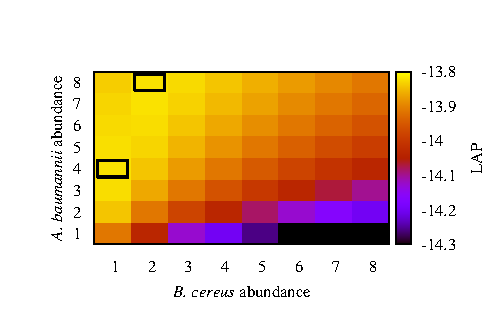
\includegraphics[width=4in]{ref_abun_1} \label{fig:ref_abun_1}}
\hfil
\subfigure[\emph{B. cereus} (4 copies, 5.2MB) and \emph{A. odontolyticus} (7 copies, 2.4MB).]{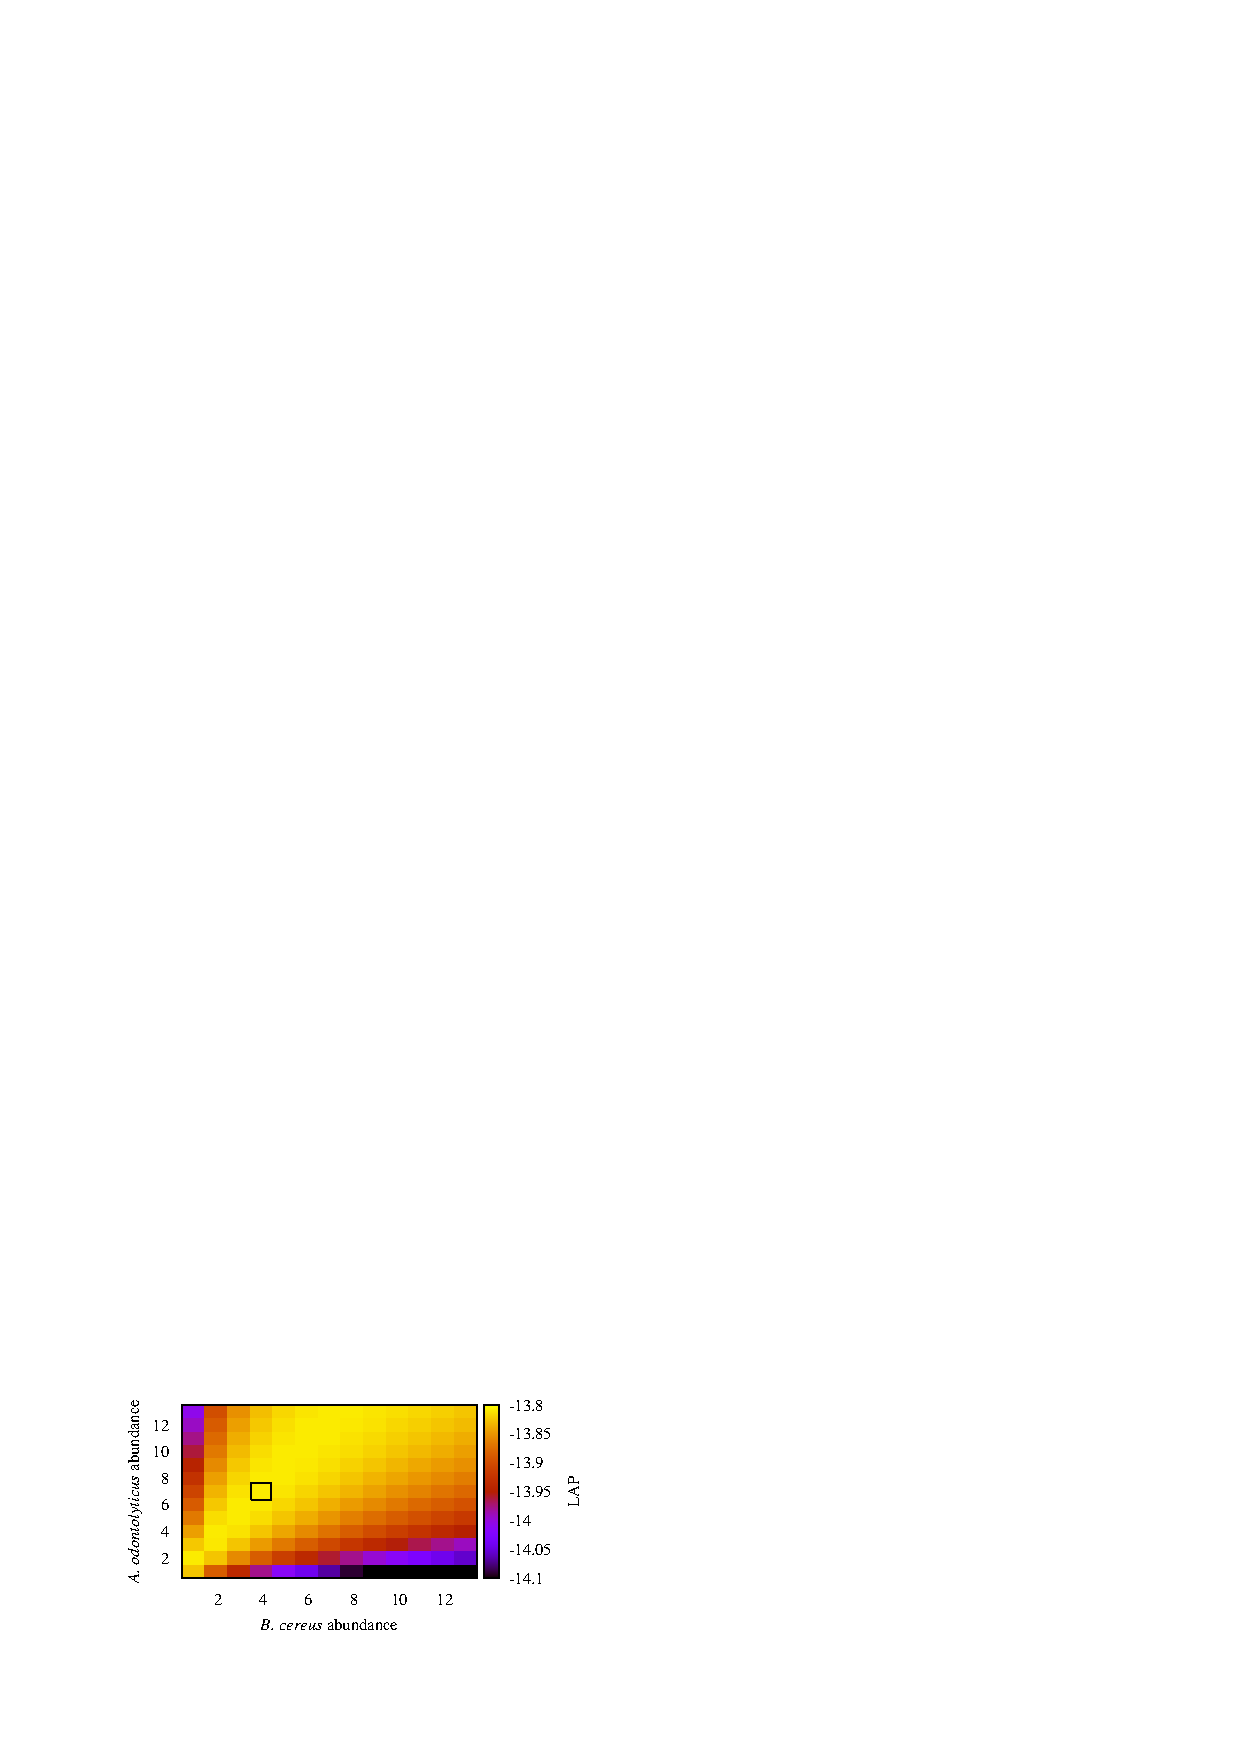
\includegraphics[width=4in]{ref_abun_2} \label{fig:ref_abun_2}}
\end{center}
\renewcommand{\baselinestretch}{1}
\small\normalsize
\begin{quote}
\caption[LAP scores for simulated metagenomic communities.] {LAP scores for simulated metagenomic communities. Each cell (x,y) represents the LAP score for a mixture of \emph{x} copies of the x-label bacteria and \emph{y} copies of the y-label bacteria.  In both groups, the true abundance ratios maximize the LAP score (indicated by a black rectangle in respective plots). \label{fig:ref_abun}}
\end{quote}
\end{figure}
\renewcommand{\baselinestretch}{2}
\small\normalsize
\newpage

\subsection{Extending LAP to metagenomic assemblies}

An important simplifying assumption of our framework is that the sequencing process is uniform in coverage.
In metagenomics, however, the relative abundances of organisms are rarely uniform~\cite{carrigg2007dna,krsek1999comparison,morgan2010metagenomic,temperton2009bias}, reflecting the difference in abundance between the different organisms within a community.
Here we show that taking this abundance information into account allows us to extend the LAP framework to metagenomic data.
%This feature makes using the LAP score incorrect out of the box.
%Later steps in the pipelines often deal with abundance estimation and phylogenetic classification.
We now assume that while the abundances of each organism may vary dramatically, the sequencing process still has uniform coverage across the \emph{entire} community.
%It is important to note while the abundances of each organism may vary dramatically, the sequencing process still produces a uniform coverage of the complete environment.
For example, consider a simple community containing two organisms (A and B), one which is twice as abundant as the other.
This community, thus, comprises twice as much of A's DNA than that of B.
Assume, for simplicity, that the community contains exactly three chromosomes (two of A and one of B).
A random sequencing process would sample each of these equally, and an ideal metagenomic assembler would produce two contigs, one covered twice as deep as the other.
%the case where we have three bacteria in an environment (1 copy of strain \emph{A}, 2 copies of strain \emph{B}).
%Now, lets assume we performed enough sequencing to produce a 1x coverage of each individual bacterium.
%An assembler would only output both bacteria strains, despite the difference in coverage.



In essence, we view the collection of individual genomes and their relative abundances as a single \emph{metagenome} where each genome is duplicated based on their abundance (\figurename \ref{fig:metagenome}).
%Thus, we now assume we have uniform coverage across the entire metagenome.
This setting is similar to that of repeats in single genome assembly, where a repetitive element can now include an entire genome.
Like in the case of single genomes, the assembler that correctly estimates these repeat counts maximizes the LAP score.
In other words, in order to accurately evaluate the metagenomic assemblies using our LAP framework, the abundance (or copy number) of each contig is needed.
%The assembler that figures out the correct copy number of repeats (in this case, contigs) will have the highest LAP score.
As most metagenomic assemblers do not report this information, 
here we use the average coverage of the contig (provided by the MetAMOS pipeline) to represent the copy number.

%In order to accurately calculate the LAP of a metagenomic assembly, in addition to the actual assemblies, we need the abundances.
In the error-free model, we compute the probability of a read, $p_r$, given the assembled sequence and abundance as:
%
\begin{equation}
  \label{meta_read_probability}
  p_r = \frac{\sum_{c \in \text{Contigs}}\text{abun}(c)*n_{rc}}{2\hat{L}}
\end{equation}
%
\begin{equation}
  \label{meta_read_length}
  \hat{L} = \sum_{c \in \text{Contigs}}\text{abun}(c)*L_{c}
\end{equation}
%
where $\text{abun}(c)$ is the abundance of contig c, $n_{rc}$ is the number of times read $r$ occurs in contig $c$, and $\hat{L}$ is the adjusted total assembly length.  In the case where the abundance of each contig is 1, calculating $p_r$ is identical to the original LAP (single genome) formulation.  A similar modification can be done to handle sequencing errors outlined in \cite{LAP}.

Our prior work has shown we can approximate the probabilities using fast and memory efficient search alignment programs (e.g., Bowtie2~\cite{langmead2012fast}) when it is impractical to calculate the exact probabilities for large read sets.
We can apply the metagenomics modification above to the alignment tool-based method:
%
\begin{equation}
\label{}
p_{r} = \frac{\sum_{j \in S_r} \text{abun}(j_{\text{contig}})*p_{r,j_{\text{subs}}}}{2\hat{L}}
\end{equation}
where $S_r$ is the set of alignments in the SAM file for the read $r$ and the probability of alignment, $p_{r,j_{\text{subs}}}$, is approximated by $\epsilon^{subs}(1 - \epsilon)^{l - subs}$ where $\epsilon$ is the probability of an error (a mismatch, an insertion, or a deletion).



%allow the assembler to tell us what copy number it expects for each contig - that is the average coverage for the contig (provided in our analysis by the MetAMOS pipeline). 
%Our LAP framework uses the average per basepair coverage of assembled contigs provided by MetAMOS.

An important factor in any likelihood-based assembly evaluation framework is the handling of reads that do not align well to the given assembly.
In practice, unalignable reads are often the result of sequencing errors and contaminants.
If these reads are given a probability close to 0, then the best assembler would be the one that incorporates the most reads.
In our original LAP framework, a read that does not align well does not decrease the overall assembly probability more than the probability of an assembly that contains the appended read as an independent contig.
This does not change when we handle metagenomic data, since the average coverage of the ``new'' contig is one.

%However, commonly used metagenomic abundance tools are often targeted at taxonomic classification~\cite{segata2012metagenomic,brady2009phymm,liu2010metaphyler,huson2007megan}.
%One strategy to estimate contig abundances is to first perform taxonomic classification on the reads and then align the contigs with the taxonomic database, transitively applying the taxonomic abundances to the contigs.
%In lieu of taxonomic abundances, our LAP framework uses the average per basepair coverage of assembled contigs provided by MetAMOS.
%We use modified version of Sailfish\cite{sailfish}, a tool to quickly calculate transcript abundances using RNA-seq data, to estimate contig abundances.
%One of the underlying assumptions of Sailfish is that the coverage

\begin{table*}[tbp]
\renewcommand{\arraystretch}{1.2}
\caption{Comparison of assembly statistics for HMP mock Even and mock Staggered datasets.\protect\footnotemark  }
\label{table_example}
\centering
\begin{tabular}{{l}{l}{c}{c}{c}{c}{c}{c}{c}{c}{c}{c}{c}}
\hline
\bfseries Dataset & \bfseries Assembler & \bfseries LAP & \bfseries \#ctgs &  \bfseries Good ctgs & \bfseries Total aln & \bfseries Slt & \bfseries Hvy & \bfseries Ch & \bfseries Size @ 10 Mbp &\bfseries Max ctg size & \bfseries Err per Mbp & \bfseries Aligned reads \\
\hline\hline

mockE & SOAPdenovo & \textbf{-27.031} & 63107 & \textbf{99.3\%} & \textbf{51} & \textbf{166} & 131          & \textbf{1} & 28,208          & 249,819          & \textbf{5.8}  & \textbf{85.75\%} \\
mockE & Velvet     & -28.537          & 12,830 & 96.2\%          & 41          & 256          & \textbf{100} & 2          & 42,269          & 179,673          & 8.7  & 83.30\%        \\
mockE & MetaVelvet & -27.102          & 22,772 & 96.8\%          & 49          & 462          & 156          & 4          & \textbf{62,138} & \textbf{367,458} & 12.7    & 85.65\%      \\
mockE & Meta-IDBA  & -31.166          & 22,032 & 95.4\%          & 47          & 362          & 151          & 3          & 26,141          & 249,069          & 11  & 81.81\%\\
\\
mockS & SOAPdenovo & -60.161          & 44,928 & \textbf{98.8\%} & \textbf{28} & 135          & 98           & \textbf{0} & 5,672           & 186,064          & \textbf{8.3} & 69.78\%  \\
mockS & Velvet     & -60.711          & 21,050 & 95.8\%          & \textbf{28} & 485          & 115          & 1          & 6,060           & 119,120          & 21.5          & 67.26\% \\
mockS & MetaVelvet & -60.442          & 20,551 & 95.3\%          & \textbf{28} & 517          & 143          & 3          & 6,685           & \textbf{217,330} & 20.1         & 67.72\% \\
mockS & Meta-IDBA  & \textbf{-58.851} & 4,559  & 92.5\%          & 18          & \textbf{101} & \textbf{83}  & \textbf{0} & \textbf{13,150} & 119,604          & 10.2  & \textbf{70.67\%}\\
\\
Tongue  & SOAPdenovo & \textbf{-13.844} & 35,230 & \textbf{89.10\%} & \textbf{11} & 1,138 & 2,618 & \textbf{0} & 11,359 & \textbf{238,051} & \textbf{341.5} & \textbf{88.14\%}\\
Tongue  & Meta-IDBA & -21.368 & 25,698 & 88.70\% & 7 & \textbf{710} & \textbf{2,087} & \textbf{0} & 4,215 & 59,188 & 399.6 & 58.89\% \\

\hline
\end{tabular}
\label{tab:hmp}
\end{table*}


\begin{figure}[b!]
\centering
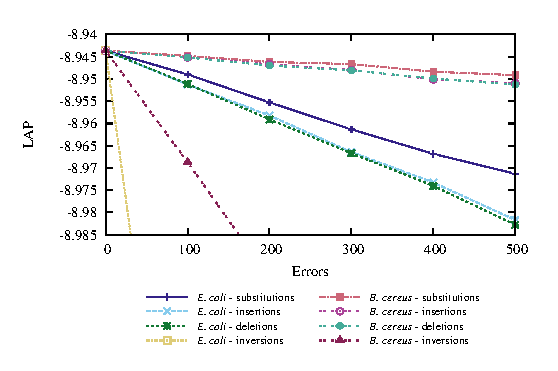
\includegraphics[width=3.5in]{errors}
\caption{Synthetic errors in simulated \emph{E. coli} (5 copies, 4.9Mbp) \emph{B. cereus} (1 copy, 5.2Mbp) community.}
\label{fig:errors}
\end{figure}


\subsection{Integration into MetAMOS}

In addition to being a standalone framework, the software implementing our metagenomic LAP approach comes packaged with the MetAMOS pipeline.
This allows users the option to run MetAMOS with different assemblers and have our framework automatically select the assembly with the highest LAP score without any prior knowledge from the user.
The first step of the MetAMOS pipeline is to \verb!Preprocess! the reads, optionally filtering out low quality reads.
Those reads are used by the next step \verb!Assemble!.
Users specify the desired assembler using the \verb!-a! parameter of \verb!runPipeline!.
We modified MetAMOS so users can now specify multiple assemblers (comma-separated) after the \verb!-a! parameter, and \verb!runPipeline! will run all assemblers and select the assembly yielding the highest LAP score to be used in downstream analyses.
%The software implementing our approach is made available, open-source and free of charge, at: \url{http://assembly-eval.sourceforge.net/} and with the MetAMOS package: \url{https://github.com/treangen/MetAMOS}.


\footnotetext{Numbers in bold represent the best value for the specific dataset.}

\section{Results}
\subsection{Likelihood score maximized using correct abundances}
A key property of our framework is that the correct copy numbers (abundances) and assemblies maximizes our LAP score.
To illustrate this property, we simulated two metagenomic communities and calculated the LAP of the reference genomes with a combination of abundances.
The first simulated community consisted of \emph{Bacillus cereus} and \emph{Acinetobacter baumannii} at a ratio of 1:4.
We generated 200bp reads at 20x coverage of the metagenome (20x of \emph{B. cereus} and 80x of \emph{A baumannii}).
We calculated the LAP scores of the error-free reference genomes for all combinations of abundances (ranging from 1 copy to 8 copies) for each bacteria.
%We calculated the LAP score on error-free reference assemblies with all combinations of abundances from 1 copy to 8 copies for each bacteria.
The second simulated community consisted of \emph{Bacillus cereus} and \emph{Actinomyces odontolyticus} at a ratio of 4:7.
We generated 200bp reads at 20x coverage of the metagenome (80x of \emph{B. cereus} and 140x of \emph{A odontolyticus}).
We calculated the LAP scores of the error-free reference genomes for all combinations of abundances (ranging from 1 copy to 13 copies) for each bacteria.


%\begin{figure}[!t]
%\centering
%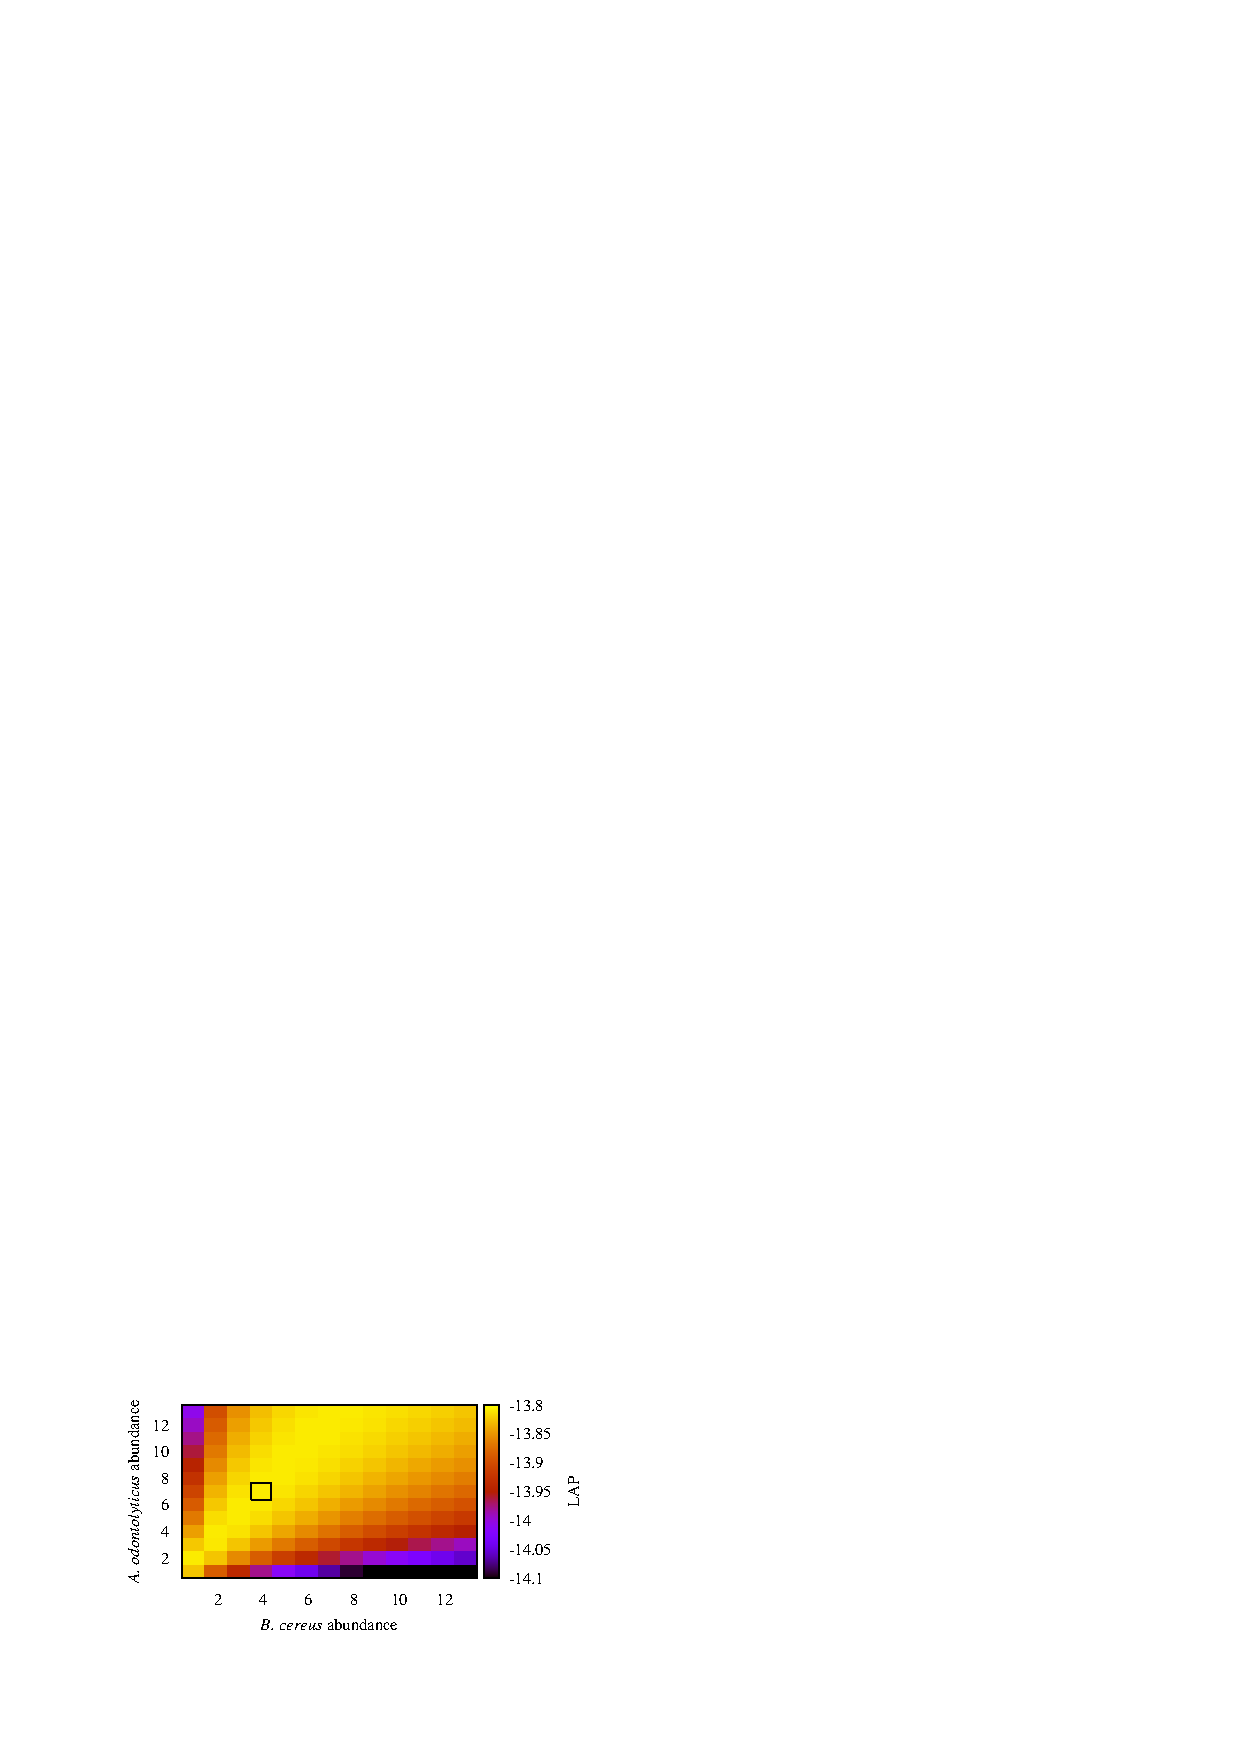
\includegraphics[width=3in]{ref_abun_2}
% where an .eps filename suffix will be assumed under latex, 
% and a .pdf suffix will be assumed for pdflatex; or what has been declared
% via \DeclareGraphicsExtensions.
%\caption{LAP scores for simulated B. cereus (4x, 5.2MB) and A. odontolyticus (7x, 2.4MB)}
%\label{fig:ref_abun_2}
%\end{figure}

We expect the highest LAP scores for the assemblies that contain the correct abundance ratios (1:4 or 2:8 in the first community, and 4:7 in the second community).
%1:4 , 2:8 boxes to be highest in figure A, and 4:7, 8:14, etc. in panel 2.  Y
As seen in Figs. \ref{fig:ref_abun_1} and \ref{fig:ref_abun_2}, our LAP score is able to accurately reflect the varying organism abundance ratios present in the sample.
The LAP score increases as the estimates approach the true abundance ratios, with the true ratio yielding the highest LAP scores in both communities.


\subsection{Impact of errors on synthetic metagenomes}

One of the often overlooked aspects of metagenomic assembly evaluation is the weighing of errors that occur in contigs with different abundances.
%In single genome assembly, errors are often not weighted since the genome has uniform coverage.
%When detecting errors with the aid of a reference, all substitution errors occurring within a genome are weighted the same (ignoring additional information, such as whether it occurs in a genic or regulatory element).
%When organism abundances are uniform, the weight of an assembly error is also uniform.
In metagenomic samples the relative organism abundances can vary by orders of magnitudes.
A typical reference-based evaluation would equally weight the errors irrespective of the abundance of the erroneous contigs.
The proposed metagenomic LAP score, however, automatically handles this situation and appropriately weighs errors according to genome abundance.
%Thus, errors in highly abundant organisms will have more of an impact on the LAP score than errors in organism of lower abundance.
To illustrate this, we simulated a small metagenomic community consisting of \emph{Escherichia coli} and \emph{Bacillus cereus} at a 5:1 ratio.
We introduced an increasing number of common assembly errors (single-base substitutions, insertions, deletions, and inversions) into the two organisms assemblies and observed the resulting LAP score.

As shown in \figurename \ref{fig:errors}, the higher the number of synthetic errors, the lower the LAP score.
Insertions/deletions were more deleterious to the LAP score than substitutions, since in addition to causing a mismatch, an insertion/deletion changes the overall genome size.
Although inversions did not change the overall genome size (and would therefore not be detected by simplistic measures such as N50), these errors had the greatest impact on the LAP score because they prevented the alignment of reads across the boundaries of the inversions.
%With substitutions and indels, reads were still able to align across the error and only incurred the additional mismatch penalty.
%Conversely, read alignment tools will fail to detect read alignments that span the borders of the inversions.

%Whereas substitutions, insertions, and deletions still allowed reads to align albeit with a lower probability, reads that inversions are essentially treated as complete

As expected, errors introduced into the more abundant organism, \emph{E. coli}, had a greater affect on the LAP score than those inserted into \emph{B. cereus}.
Our LAP score was able to accurately weigh the errors by the abundance of each organism.


\subsection{Likelihood scores correlate with reference-based metrics}
%c|c|c|c|c|c


With real metagenomic samples, it is difficult to make evaluations given the lack of high quality references.
Using purely simulated data has the issue of not accurately capturing the error and bias introduced by sequencing technology.
Thus, to evaluate our LAP score, we use two `mock' communities (Even and Staggered) provided by the Human Microbiome Project (HMP) consortium\cite{mitreva2012structure,methe2012framework}.
These communities were created using specific DNA sequences from organisms with known reference genomes (consisting of over 20 bacterial genomes and a few eukaryotes) and abundances.
The mock Even community consisted of 100,000 16S copies per organism per aliquot, while the mock Staggered community consisted of 1,000 to 1,000,000 16S copies per organism per aliquot.
Data used from the HMP mock communities are available at \url{http://www.ncbi.nlm.nih.gov/bioproject/48475}.
We calculated the LAP score on assemblies produced by MetAMOS~\cite{treangen2013metamos} using several assemblers: SOAPdenovo~\cite{SOAPdenovo}, Metavelvet~\cite{namiki2012metavelvet}, Velvet~\cite{Velvet}, and Meta-IDBA~\cite{peng2011meta}.
The additional \emph{de novo} and reference-based metrics for the assemblies were taken from MetAMOS~\cite{treangen2013metamos}.  These metrics include:
   \begin{itemize}
   \item number contigs (\# ctgs) -- total number of contigs/scaffolds in the assembly
   \item good contigs (Good Ctgs) -- fraction of contigs that mapped without errors to reference genomes
   \item total aligned (Total aln) -- total amount of sequence (in Mbp) that can be aligned to the reference genomes
   \item slight mis-assemblies (Slt) -- alignments that cover 80\% or more of the aligned contig in a single match (Slt)
   \item heavy misassemblies (Hvy) -- alignments that cover less than 80\% of the aligned contig in a single match or have two or more matches to a single reference
   \item chimeras (Ch) -- contigs with matches to two distinct reference genomes
   \item size at 10 megabases (Size @ 10 Mbp) - the size of the largest contig $c$ such that the sum of all contigs larger than $c$ is more than 10 Mbp (similar to the commonly used N50 size)
   \item max contig size (Max ctg size) -- size of the largest contig in the assembly
   \item errors per megabase (Err per Mbp) -- average number of errors per Mbp in the assembly
   \end{itemize}

Generally, the \emph{de novo} LAP scores agree with the referenced-based metrics (Table \ref{tab:hmp}).
In the mock Even dataset, SOAPdenovo has the greatest LAP score, the highest fraction of contigs that can align to a reference genome without error, total amount of sequence that can be aligned to a reference genome, while also having the lowest amount of misassemblies (including chimeric) and errors per Mbp.
It is important to note that if user selected an assembly based on the best contiguity at 10Mbp, they would select the MetaVelvet assembly, which contains double the error rate per Mbp as the SOAPdenovo assembly while aligning 2Mbp less to the references.

Since the abundances of each organism in the mock Even dataset are fairly similar, the mock Staggered abundance distribution creates a more realistic scenario encountered in metagenomic environments.
Here, the Meta-IDBA assembly has the greatest LAP score, but aligns roughly a third less sequences to the reference genomes than SOAPdenovo.
The Meta-IDBA assembly contains approximately a tenth of the amount of contigs (4,559 vs. 44,928) as SOAPdenovo.
The SOAPdenovo assembly contains a greater number of contigs at a very low abundance (\figurename \ref{fig:coverage}).
On large contigs Meta-IDBA performs better than SOAPdenovo and has a lower error rate (see \figurename 4 in \cite{treangen2013metamos}).
However, Meta-IDBA assembles a smaller fraction of the low-abundance genomes than SOAPdenovo, leading fewer sequences to align.
The LAP score penalizes misassemblies within abundant contigs in the SOAPdenovo results.


%Given how the mock Staggered community was constructed (each ratio of 16S copies per aliquot occurred roughly the same number of times), the frequency of contig abundances should be approximately uniform for the community.
%The SOAPdenovo assembly was able to align more reads, but the reads were localized in these low coverage regions.
%The distribution of contig abundances in the Meta-IDBA assembly was closer to the expected distribution than the SOAPdenovo assembly.

%The Meta-IDBA assembly a far more uniform frequency of contig abundances compared to the SOAPdenovo assembly.

Next, we applied our framework on real data where we did not know the actual genomes comprising the sample (HMP tongue dorsum female sample, SRS077736) (Table \ref{tab:hmp}).
Although we do not know for certain which organisms are present in the sample, the HMP identified a reference genome set with high similarity to the sequences within the sample (HMP Shotgun Community profiling SRS077736). 
The reference-based error metrics only consider chimeric errors due to the possibility of structural difference between an organism and its version in the reference database.
We calculated the LAP of the assemblies using a single library consisting of 42,013,917 reads.
The SOAPdenovo assembly had a far greater LAP score than the Meta-IDBA assembly.
The higher score is due to the SOAPdenovo assembly recruiting more reads (88.14\% to 58.89\%) in relation to its genome size (46Mbp to 37Mbp) than the Meta-IDBA assembly.
Furthermore, the MetAMOS metrics show that the SOAPdenovo assembly contained approximately 60 less errors per Mbp than the Meta-IDBA assembly.

%These datasets have the advantage over simulated data because it captures the error and bias introduced from the sequence technology.



\begin{figure}[tb!]
\centering
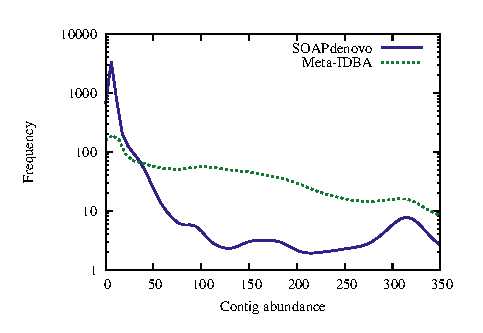
\includegraphics[width=3in]{coverage}
\caption{Frequency of contig abundances for assemblies of the HMP mock Staggered dataset.}
\label{fig:coverage}
\end{figure}


\begin{table}[b]
\caption{Self-tuning MetAMOS using \emph{C. ruddii} test dataset.}
\label{tab:metamos_lap}
\centering
\begin{tabular}{{l}{c}{c}{c}{c}}
\hline
\bfseries Assembler & \bfseries Contigs & \bfseries LAP & \bfseries N50 (Kbp) & \bfseries  Errors \\
\hline \hline
newbler  & \bf{1} & \bf{-13.064} & \bf{156} & 1 \\
SOAPdenovo & 23 & -14.238 & 9 & \bf{3} \\
Velvet & 3 & -13.157 & 92 & \bf{0} \\
MetaVelvet & 3 & -13.157 & 92 & \bf{0} \\
\hline
\end{tabular}
\end{table}



\subsection{Tuning assembly parameters for MetAMOS}
Assemblathon1~\cite{earl2011assemblathon} has shown that assembly experts can often get drastically different assemblies using the same assemblers, highlighting the difficulty of choosing the \emph{right} parameters for a given assembler.
Our metagenomic LAP framework comes packaged with the MetAMOS pipeline, allowing users the option to run MetAMOS with different assemblers and automatically select the assembly with the highest LAP score.
This step occurs without any prior knowledge from the user.

We showcase the ease of use of the automated assembler selection within MetAMOS using the \emph{Carsonella ruddii} (156Kbp) dataset packaged with MetAMOS (Table ~\ref{tab:metamos_lap}).
Errors were found using DNADIFF~\cite{phillippy2008genome} and MUMmer~\cite{delcher2003using}.
The newbler assembly produced one contig containing the complete \emph{C. ruddii} genome.
The SOAPdenovo assembly produced a severely fragmented assembly with the most number of errors.
The MetaVelvet and Velvet produced identical assemblies, containing 3 contigs of sizes 92Kbp, 65Kbp, and 1.7Kbp, but contained an additional 158bp compared to the \emph{C. ruddii} genome.
Upon closer inspection, there were overlaps between the contigs ranging from 38bp to 73bp.
This is not surprising given MetaVelvet's and Velvet's de bruijn graph-based approach could not resolve repetitive regions between the contigs.
Newbler, on the other hand, contained only a single insertion error.
The LAP score of the Newbler assembly was greater due to more reads being able to align across the regions that were broken apart in the MetaVelvet and Velvet assemblies.
Additionally, the Newbler assembly did not contain the duplicated sequence found in the other assemblies.
MetAMOS was able to select the most likely assembly without requiring any additional input from the user.

\section{Discussion}

In this paper, we have proposed an extension to our LAP framework to perform \emph{de novo} comparisons of metagenomic assemblies.
Unlike traditional \emph{de novo} metrics used for measuring assembly quality, our extended LAP score correlates well with reference-based measures of metagenomic assembly quality.
However, in this study, we have realized that there is a lack of reference-based metrics when evaluating metagenomic assemblies.
Misjoins betweens organisms may be more deleterious than misjoins within a single genome.
Furthermore, current reference-based metrics do not take into account the relative abundances of the organisms when evaluating metagenomic assemblies.
The metrics provided by MetAMOS do not factor in the contig abundances when examining assembly errors.
This made it difficult to compare our LAP score to their reference-based metrics because, intuitively, an error in a highly abundant organism should be \emph{worse} than an error in a rare, low coverage organism.
Our LAP score implicitly weighs the errors in abundant contigs more than those in lesser abundant contigs.
In our results, we have proposed one such reference-based metric that scales the errors by the relative abundance of the contig it occurs within.

It is important to note that we have only focused on the complete reconstruction of the metagenome from the set of reads.
Assembly algorithms are designed with specific biological applications in mind, such as, the conservative reconstruction of the genic regions.
Studies focusing on the genic regions may tolerate large-scale rearrangements as long as the genic regions were correctly assembled.
Conversely, other studies may want to focus on the reconstruction and detection of rare pathogenic bacteria in an environment.
These application specific assembly algorithms all attempt to optimize their formulation of the assembly problem.

Our metagenomic LAP extension relies heavily on the idea that the sequencing process of the metagenome is roughly uniform, and that the reads are independently sampled from the genome.
Biases exist in all steps of the sequencing process, from the extraction of DNA from organisms with different cell membranes/walls~\cite{carrigg2007dna,krsek1999comparison} to the sequencing protocol used~\cite{morgan2010metagenomic,temperton2009bias}.
In the future, we would like to implement a more specific model that better captures the sequencing process.

%De novo metric, more misleading in assemblies -> chimera

%We would like to stress that \emph{de novo} measures of assembly quality, such as ours, are critically needed by researchers attempting to assemble of yet unknown genomes.

Results from GAGE~\cite{salzberg2011gage} and Assemblathon~\cite{earl2011assemblathon,bradnam2013assemblathon} have shown that the specific characteristics of the data being assembled has a great impact on the performance of the assembler.
This problem is magnified in metagenomic assembly.
By integrating our LAP framework in MetAMOS, we have allowed researchers to accurately and effortlessly run and evaluate assemblies without any prior knowledge on evaluating assembly quality.

In our framework, we use the average coverage of the contig (provided by MetAMOS) to estimate abundance.
There are issues with this measure as it is possible that mis-assembled repeats within a contig will affect our estimate of depth of coverage and could impact our underlying statistics.
A better approach is to use something more robust than the mean coverage, such as the median coverage, to avoid being influenced by such regions.
While the user can supply the median coverage to our standalone framework, future work includes building this feature into MetAMOS.
Another approach involves breaking contigs at regions of differing coverage (using tools such as AMOSvalidate\cite{phillippy2008genome}), so there will be less deviation in the average coverage within the contig.

It should be noted that in some cases it may not be tractable to run the complete collection of assemblers with MetAMOS.
In such cases, we should first employ heuristics (such as \cite{chikhi2013informed}) to aid in selecting potential assemblers (and parameters) to run.
For the assembler selection process, we can use the LAP framework's sampling procedure in combination with calculating read probabilities in parallel to reduce runtime.

Our goal was to provide a global measure of how good a metagenomic assembly may be, not to detect assembly errors.
Other likelihood-based frameworks, such as ALE, use frequencies of certain sequences to aid in detection of possible chimeric contigs.
We are able to apply similar modifications to our LAP framework to find regions of possible misassembly.
Finally, we plan to extend our framework to give a more detailed breakdown of the LAP scores of segments assembled using the same subset of reads across different assemblies.
The goal would be to take high-scoring assembled segments from individual assemblies to recreate an assembly with overall greater likelihood.
This approach will be of great benefit to the field of metagenomic assembly since assemblers are often designed with different constraints and goals in mind, e.g., low memory footprint, assembling high/low coverage organisms, or tolerating population polymorphisms.
For example, on the mock Staggered dataset, Meta-IDBA best assembled the most abundant genomes while SOAPdenovo had a better representation of the low abundance organisms.
Providing a systematic way of combining assembler approaches using our LAP score will produce better assemblies for downstream analyses.


% An example of a floating figure using the graphicx package.
% Note that \label must occur AFTER (or within) \caption.
% For figures, \caption should occur after the \includegraphics.
% Note that IEEEtran v1.7 and later has special internal code that
% is designed to preserve the operation of \label within \caption
% even when the captionsoff option is in effect. However, because
% of issues like this, it may be the safest practice to put all your
% \label just after \caption rather than within \caption{}.
%
% Reminder: the "draftcls" or "draftclsnofoot", not "draft", class
% option should be used if it is desired that the figures are to be
% displayed while in draft mode.
%
%\begin{figure}[!t]
%\centering
%\includegraphics[width=2.5in]{myfigure}
% where an .eps filename suffix will be assumed under latex, 
% and a .pdf suffix will be assumed for pdflatex; or what has been declared
% via \DeclareGraphicsExtensions.
%\caption{Simulation Results}
%\label{fig_sim}
%\end{figure}

% Note that IEEE typically puts floats only at the top, even when this
% results in a large percentage of a column being occupied by floats.


% An example of a double column floating figure using two subfigures.
% (The subfig.sty package must be loaded for this to work.)
% The subfigure \label commands are set within each subfloat command, the
% \label for the overall figure must come after \caption.
% \hfil must be used as a separator to get equal spacing.
% The subfigure.sty package works much the same way, except \subfigure is
% used instead of \subfloat.
%
%\begin{figure*}[!t]
%\centerline{\subfloat[Case I]\includegraphics[width=2.5in]{subfigcase1}%
%\label{fig_first_case}}
%\hfil
%\subfloat[Case II]{\includegraphics[width=2.5in]{subfigcase2}%
%\label{fig_second_case}}}
%\caption{Simulation results}
%\label{fig_sim}
%\end{figure*}
%
% Note that often IEEE papers with subfigures do not employ subfigure
% captions (using the optional argument to \subfloat), but instead will
% reference/describe all of them (a), (b), etc., within the main caption.


% An example of a floating table. Note that, for IEEE style tables, the 
% \caption command should come BEFORE the table. Table text will default to
% \footnotesize as IEEE normally uses this smaller font for tables.
% The \label must come after \caption as always.
%
%\begin{table}[!t]
%% increase table row spacing, adjust to taste
%\renewcommand{\arraystretch}{1.3}
% if using array.sty, it might be a good idea to tweak the value of
% \extrarowheight as needed to properly center the text within the cells
%\caption{An Example of a Table}
%\label{table_example}
%\centering
%% Some packages, such as MDW tools, offer better commands for making tables
%% than the plain LaTeX2e tabular which is used here.
%\begin{tabular}{|c||c|}
%\hline
%One & Two\\
%\hline
%Three & Four\\
%\hline
%\end{tabular}
%\end{table}


% Note that IEEE does not put floats in the very first column - or typically
% anywhere on the first page for that matter. Also, in-text middle ("here")
% positioning is not used. Most IEEE journals/conferences use top floats
% exclusively. Note that, LaTeX2e, unlike IEEE journals/conferences, places
% footnotes above bottom floats. This can be corrected via the \fnbelowfloat
% command of the stfloats package.



\section{Conclusion}
In this paper we have described an extension to our \emph{de novo} assembly evaluation framework (LAP) for comparing metagenomic assemblies.
We showed that the true metagenome and correct relative abundances maximizes our extended LAP score.
Furthermore, we have integrated our framework into the metagenomic assembly pipeline MetAMOS, showing that any user is able to reproduce quality evaluations of metagenomic assemblies with relative ease.



%Chapter 2

\renewcommand{\thechapter}{3}

\chapter{Comparing Metagenomic Assemblies}
%
% \section{Abstract}
% %\boldmath
% The ever-decreasing costs of sequencing technology has led to a sharp increase in metagenomics projects over the past decade, allowing us to better understand the diversity and function of microbial communities found in the world around us.
% The first step in these analyses is to perform
% genome assembly to piece together the DNA fragments into complete, or
% near complete, genomes.
% %The first step in these analyses involves the use of tools called assemblers that piece together the DNA fragments into complete or near complete genome sequences.
% Metagenomic assemblers inherit all the difficulties of traditional single genome assembly, but with the additional complexity of trying to resolve assemblies of closely related species with drastically varying abundances.
% Assessing and comparing the quality of single genome assembly still relies on the availability of independently determined standards, such as manually curated genomic sequences.
% These standards are often not possible in metagenomic projects, where a large portion of the organisms and strains are novel.
% Thus, we must rely on \emph{de novo} methods for assessing and comparing assembly qualities.
% Here we describe an extension to our \emph{de novo} LAP framework to evaluate metagenomic assemblies.
% We will show that by modifying our likelihood calculation to take into account abundances of assembled sequences, we can accurately and efficiently compare metagenomic assemblies.
% %We evaluate our extended framework on results generated from the Human Microbiome Project (HMP) and
% We find that our extended LAP framework is able to reproduce results on data from the Human Microbiome Project (HMP) that closely match the reference-based evaluation metrics and outperforms other \emph{de novo} metrics traditionally used to measure assembly quality.
% Finally, we have integrated our LAP framework into the metagenomic analysis pipeline MetAMOS, allowing any user to reproduce quality assembly evaluations with relative ease.
% %Even without knowledge of the true reference sequences, our \emph{de novo} metric
% %Here we introduce an extension to our LAP  \emph{de novo} probabilistic measure of assembly quality, which allows for an objective comparison of multiple assemblies generated from the same set of reads.
% %We define the quality of a sequence produced by an assembler, as the conditional probability of observing the sequenced reads from the assembled sequence.
%

\section{Introduction}
% The genome sequence of an organism is a vital resource for biologists trying to better understand its function and evolution.
% Generating this sequence is not an easy task as modern sequencing technologies can only ``read'' small pieces of the genome.
% These sequences, known as \emph{reads}, have to be pieced together by tools called assemblers using a collection of different heuristics since in almost all practical cases, assemblers cannot fully and accurately reconstruct the genome~\cite{myers1995,medvedev2007computability}.
%
% Practical implementations of assembly algorithms (such as ABySS~\cite{ABySS}, SOAPdenovo~\cite{SOAPdenovo}, Velvet~\cite{Velvet}, etc.) return just an approximate solution that is often fragmented and contains numerous errors.
% Ideally, further experiments would be performed manually to correct the hundreds to thousands of errors~\cite{salzberg2005misassemblies}, and fill in the gaps between the chunks of assembled sequences (called contigs)~\cite{nagarajan2010finishing}.
% However, the additional cost and effort necessary to finish a genome is only justifiable for a few high-priority organisms (typically model organisms).
% Recent technology advances have demonstrated automatically assembled finish-grade quality bacterial genomes~\cite{chin2013nonhybrid, koren2013reducing, ribeiro2012finished}. However, the majority of genomes sequences available today are considered to be in a ``draft'' state, with no clear indication of their respective quality, possibly impacting the conclusions and experiments done on their sequences.

Despite the unresolved challenges of clonal genome assembly, the decreasing costs of sequencing technology has led to a sharp increase in metagenomics projects over the past decade.
% have been sharply on the rise over the past decade,
These projects allow us to better understand the diversity and function of microbial communities found in the environment, including the ocean\cite{rusch2007sorcerer,wu2011stalking,yooseph2007sorcerer}, Arctic regions \cite{varin2012metagenomic}, other living organisms\cite{he2013comparative} and the human body\cite{gill2006metagenomic,peterson2009nih}.
Traditional \emph{de novo} genome assemblers have trouble assembling these datasets due to the presence of closely related species and and the need to distinguish between true polymorphisms and errors arising from the sequencing technology.
Metagenomic assemblers often use heuristics based on sequencing (Meta-IDBA \cite{peng2011meta} and MetaVelvet\cite{namiki2012metavelvet}) and k-mer (Ray Meta \cite{boisvert2012ray}) coverage to split the assembly graph into subcomponents that represent different organisms, then apply traditional assembly algorithms on the individual organisms.

As the number of metagenomic assemblers available to researchers continues to increase, the development of approaches for validating and comparing the output of these tools is of critical importance.
Despite the incremental improvements in performance, none of the assembler tools available today outperforms the rest in all cases (as highlighted by recent assembly
bake-offs GAGE\cite{salzberg2011gage} and Assemblathons 1~\cite{earl2011assemblathon} and 2~\cite{bradnam2013assemblathon}).
Different assemblers ``win'' depending on the specific downstream analyses, structure of the genome, and sequencing technology used.
These competitions highlight the inherent difficulty of assessing assembly quality -- where do you set the line between increased contiguity and decreasing accuracy of the resulting sequence?
Evaluating the trade-off between increased contiguity and errors is difficult even when there is a gold standard reference genome to compare to, which is not available in most practical assembly cases.
Thus, we are forced to heavily rely on \emph{de novo} approaches based on sequence data alone.
% (including global ``sanity checks,'' such as gene density, which is expected to be high in bacterial genomes).

One objective \emph{de novo} metric, that has been used to evaluate and compare assembly quality, is based on the likelihood that the observed reads are generated from the given assembly, which can be accurately estimated by modeling the sequencing process.
This metric was proposed by Gene Myers in his pioneering work in the 1990's, where he suggested that the correct assembly must be consistent with the statistical properties of the data generation process.
This idea was extended and used by recent assembly evaluation frameworks: ALE ~\cite{clark2013ale}, CGAL~\cite{rahman2013cgal}, and LAP~\cite{LAP}.

%In pioneering work in the 1990's, Gene Myers suggested that the correct assembly given the set of reads must be consistent with the data generation process.
%This idea was extended and used by assemblers and assembly evaluation software: the arrival-rate statistic (A-statistic) in Celera
%assembler~\cite{CeleraAssembler} to identify collapsed repeats, and
%as an objective function in quasi-species (ShoRAH~\cite{SHORAH},
%ViSpA~\cite{VISPA}), metagenomic (Genovo~\cite{genovo2011}),
%general-purpose assemblers~\cite{medvedev2009maximum}, and recent assembly
%evaluation frameworks.

Most of the previous \emph{de novo} and reference-based validation methods have been designed for single genome assembly.
Currently, there are no universally-accepted reference-based metrics for evaluating metagenomic assemblies.
Despite reference sequences being available for a small fraction of organisms found in metagenomic environments \cite{angly2006marine,dinsdale2008functional}, it is not clear how to distinguish errors from genomic variants found within a population.
%In addition to chimeric contigs within a single organism, there are now potential chimeras that span multiple organisms.
Furthermore, it is not clear how to weigh errors occurring in more abundant organisms.
Likelihood-based frameworks, such as ALE ~\cite{clark2013ale}, CGAL~\cite{rahman2013cgal}, and LAP~\cite{LAP}, rely on the assumption that the sequencing process is approximately uniform across the genome; however, the sequencing depth across genomes in metagenomic samples can vary greatly~\cite{carrigg2007dna,krsek1999comparison,morgan2010metagenomic,temperton2009bias}.

%Assessing the quality of the sequence output by an assembler is of critical importance for downstream analyses and allows researchers to choose from a collection of genome assembler.

In this chapter, we describe an extension to our LAP framework to evaluate metagenomic assemblies.
We will show that by modifying our likelihood calculation to take into account contig abundances, we can accurately and efficiently evaluate metagenomic assemblies.
We evaluate our extended framework on data from the Human Microbiome Project (HMP).
Finally, we show how our LAP framework can be used automatically by the metagenomic assembly pipeline, MetAMOS\cite{treangen2013metamos}, to select the best assembler for a specific dataset, and to provide users with a measure of assembly quality.
The software implementing our approach is made available, open-source and free of charge, at: \url{http://assembly-eval.sourceforge.net/} and with the MetAMOS package: \url{https://github.com/treangen/MetAMOS}.

%\hfill mds

%\hfill July 17, 2013

%\newpage
\begin{figure}
\begin{center}
\includegraphics[width=4.572in]{metagenome}
\end{center}
\renewcommand{\baselinestretch}{1}
\small\normalsize
\begin{quote}
\caption[The metagenome of an environment]{The metagenome of an environment can be viewed as the concatenation of the organisms found in the environment whose multiplicity is determined by their abundance. \label{fig:metagenome}}
\end{quote}
\end{figure}
\renewcommand{\baselinestretch}{2}
\small\normalsize
\newpage

% \begin{figure}[!t]
% \centering
% \includegraphics[width=3in]{metagenome}
% % where an .eps filename suffix will be assumed under latex,
% % and a .pdf suffix will be assumed for pdflatex; or what has been declared
% % via \DeclareGraphicsExtensions.
% \caption{The metagenome of an environment can be viewed as the concatenation of the organisms found in the environment whose multiplicity is determined by their abundance.}
% \label{fig:metagenome}
% \end{figure}


\section{Methods}
% \subsection{Likelihood of an assembly}
%
% Our LAP framework measures the quality of an assembly as the probability that the observed reads, $R$, are generated from the given assembly, $A$: $\Pr[R|A]]$ \cite{LAP}.
% Assuming that the event of observing each read is independent, then the probability $\Pr[R|A]$ of the read set $R$ being produced from the assembly $A$, is the product of the individual read probabilities, $p_r$.  That is,
% \begin{equation}
%   \label{probability_reads_given_assembly}
%   \Pr[R \vert A]=\prod_{r \in R} p_r
% \end{equation}
%
% By modeling the data generation process, we can calculate the probability of each read, $p_r$.
% Assuming uniform coverage, where each position in the genome is covered by roughly the same amount of reads as any other position, a read may be sequenced starting from any position of the genome with equal probability.
% In the basic error-free model, if a read matches to one position in the assembly, and its reverse-complement does not match anywhere, then the probability of the read being produced from the assembly is $p_r=\frac{1}{2L}$, where $L$ is the length of the assembly.
% The length of the assembly is doubled due to the double-stranded molecules of DNA that make up the genome.
% Thus, if a read
% %and its reverse-complement
% matches at $n_r$ positions on the assembly, then
% % and its reverse-complement
% \begin{equation}
%   \label{error_free_probability}
%   p_r = \frac{n_r}{2L}
% \end{equation}
%
% Ghodsi et. al.~\cite{LAP} detail how to modify the calculation of $p_r$ to handle practical constraints, e.g., sequencing errors and mate pairs.
% They also show that the true genome maximizes $\Pr[R|A]$.
%
% %The metric used in accessing the assembly probability is the logarithm of the geometric mean of the read probabilities, referred to as the log average probability (LAP).
% Calculating $\Pr[R|A]$ can be expensive for dataset sizes commonly encountered in sequencing projects (tens to hundreds of millions of reads).
% Thus, we can approximate the likelihood of the assembly by using a random subset of the reads ($R^\prime$).
% To counteract the effect of sample size on the probability, we define the assembly quality as the geometric mean of the read probabilities:
% %
% \begin{align}
% \label{average_log_probability}
%   \operatorname{AP}(R^\prime) =
%   \left(\prod_{r \in R^\prime} p_r\right)^{\frac{1}{\left|R^\prime\right|}} \nonumber  \\
%   \operatorname{LAP}(R^\prime) = \log_{10} \left( \operatorname{AP}(R^\prime) \right) = \frac{\sum_{r \in R^\prime} \log_{10} p_r}{\left|R^\prime\right|}
% \end{align}
% %
% %For the remainder of this paper, we define the assembly quality as the average log likelihood (LAP) of the reads given the assembly.
% %This formulation allows us to estimate the
% The mean of the read probabilities over the sample is expected to be equal to the mean over all reads, but if the sample size is too small, then the accuracy of the estimation will be poor.

\begin{figure}
\begin{center}
%\begin{figure*}[tbhp!]
%\centering

\subfigure[\emph{B. cereus} (1 copy, 5.2MB) and \emph{A. baumannii} (4 copies, 4.0MB)]{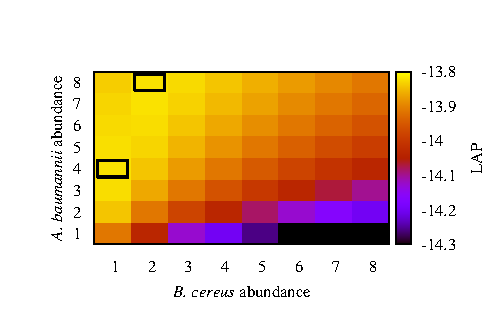
\includegraphics[width=4in]{ref_abun_1} \label{fig:ref_abun_1}}
\hfil
\subfigure[\emph{B. cereus} (4 copies, 5.2MB) and \emph{A. odontolyticus} (7 copies, 2.4MB)]{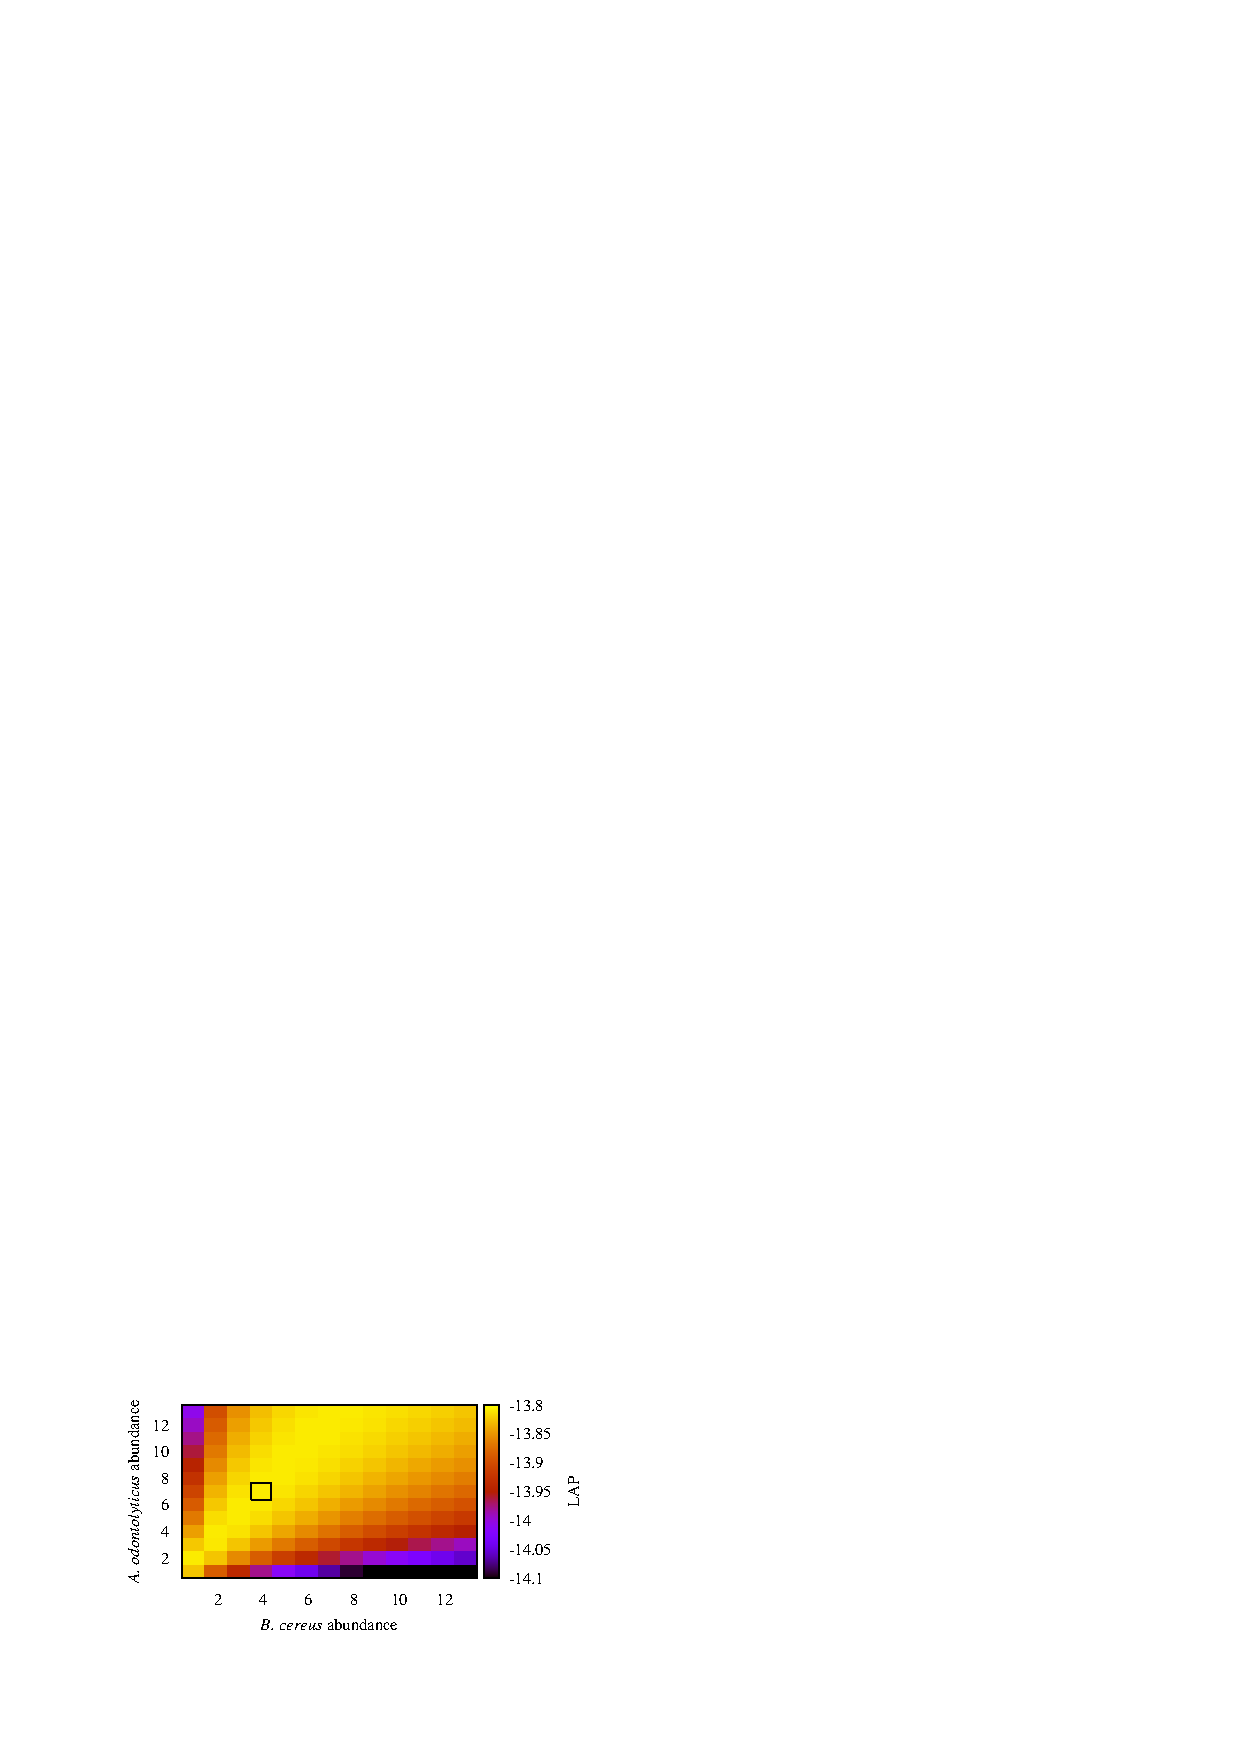
\includegraphics[width=4in]{ref_abun_2} \label{fig:ref_abun_2}}
\end{center}
\renewcommand{\baselinestretch}{1}
\small\normalsize
\begin{quote}
\caption[LAP scores for simulated metagenomic communities.] {LAP scores for simulated metagenomic communities. Each cell (x,y) represents the LAP score for a mixture of \emph{x} copies of the x-label bacteria and \emph{y} copies of the y-label bacteria.  In both groups, the true abundance ratios maximize the LAP score (indicated by a black rectangle in respective plots). \label{fig:ref_abun}}
\end{quote}
\end{figure}
\renewcommand{\baselinestretch}{2}
\small\normalsize
\newpage

\subsection{Extending LAP to metagenomic assemblies}

An important simplifying assumption of our framework is that the sequencing process is uniform in coverage.
In metagenomics, however, the relative abundances of organisms are rarely uniform~\cite{carrigg2007dna,krsek1999comparison,morgan2010metagenomic,temperton2009bias}, reflecting the difference in abundance between the different organisms within a community.
Here we show that taking this abundance information into account allows us to extend the LAP framework to metagenomic data.
%This feature makes using the LAP score incorrect out of the box.
%Later steps in the pipelines often deal with abundance estimation and phylogenetic classification.
We now assume that while the abundances of each organism may vary dramatically, the sequencing process still has uniform coverage across the \emph{entire} community.
%It is important to note while the abundances of each organism may vary dramatically, the sequencing process still produces a uniform coverage of the complete environment.
For example, consider a simple community containing two organisms (A and B), one which is twice as abundant as the other.
This community, thus, comprises twice as much of A's DNA than that of B.
Assume, for simplicity, that the community contains exactly three chromosomes (two of A and one of B).
A random sequencing process would sample each of these equally, and an ideal metagenomic assembler would produce two contigs, one covered twice as deep as the other.
%the case where we have three bacteria in an environment (1 copy of strain \emph{A}, 2 copies of strain \emph{B}).
%Now, lets assume we performed enough sequencing to produce a 1x coverage of each individual bacterium.
%An assembler would only output both bacteria strains, despite the difference in coverage.



In essence, we view the collection of individual genomes and their relative abundances as a single \emph{metagenome} where each genome is duplicated based on their abundance (\figurename~\ref{fig:metagenome}).
%Thus, we now assume we have uniform coverage across the entire metagenome.
This setting is similar to that of repeats in single genome assembly, where a repetitive element can now include an entire genome.
Like in the case of single genomes, the assembler that correctly estimates these repeat counts maximizes the LAP score.
In other words, in order to accurately evaluate the metagenomic assemblies using our LAP framework, the abundance (or copy number) of each contig is needed.
%The assembler that figures out the correct copy number of repeats (in this case, contigs) will have the highest LAP score.
As most metagenomic assemblers do not report this information,
here we use the average coverage of the contig (provided by the MetAMOS pipeline) to represent the copy number.

%In order to accurately calculate the LAP of a metagenomic assembly, in addition to the actual assemblies, we need the abundances.
In the error-free model, we compute the probability of a read, $p_r$, given the assembled sequence and abundance as:
%
\begin{equation}
  \label{meta_read_probability}
  p_r = \frac{\sum_{c \in \text{Contigs}}\text{abun}(c)*n_{rc}}{2\hat{L}}
\end{equation}
%
\begin{equation}
  \label{meta_read_length}
  \hat{L} = \sum_{c \in \text{Contigs}}\text{abun}(c)*L_{c}
\end{equation}
%
where $\text{abun}(c)$ is the abundance of contig c, $n_{rc}$ is the number of times read $r$ occurs in contig $c$, and $\hat{L}$ is the adjusted total assembly length.  In the case where the abundance of each contig is 1, calculating $p_r$ is identical to the original LAP (single genome) formulation.  A similar modification can be done to handle sequencing errors outlined in \cite{LAP}.

Our prior work has shown we can approximate the probabilities using fast and memory efficient search alignment programs (e.g., Bowtie2~\cite{langmead2012fast}) when it is impractical to calculate the exact probabilities for large read sets.
We can apply the metagenomics modification above to the alignment tool-based method:
%
\begin{equation}
\label{}
p_{r} = \frac{\sum_{j \in S_r} \text{abun}(j_{\text{contig}})*p_{r,j_{\text{subs}}}}{2\hat{L}}
\end{equation}
where $S_r$ is the set of alignments in the SAM file for the read $r$ and the probability of alignment, $p_{r,j_{\text{subs}}}$, is approximated by $\epsilon^{subs}(1 - \epsilon)^{l - subs}$ where $\epsilon$ is the probability of an error (a mismatch, an insertion, or a deletion).



%allow the assembler to tell us what copy number it expects for each contig - that is the average coverage for the contig (provided in our analysis by the MetAMOS pipeline).
%Our LAP framework uses the average per basepair coverage of assembled contigs provided by MetAMOS.

An important factor in any likelihood-based assembly evaluation framework is the handling of reads that do not align well to the given assembly.
In practice, unalignable reads are often the result of sequencing errors and contaminants.
If these reads are given a probability close to 0, then the best assembler would be the one that incorporates the most reads.
In our original LAP framework, a read that does not align well does not decrease the overall assembly probability more than the probability of an assembly that contains the appended read as an independent contig.
This does not change when we handle metagenomic data, since the average coverage of the ``new'' contig is one.

%However, commonly used metagenomic abundance tools are often targeted at taxonomic classification~\cite{segata2012metagenomic,brady2009phymm,liu2010metaphyler,huson2007megan}.
%One strategy to estimate contig abundances is to first perform taxonomic classification on the reads and then align the contigs with the taxonomic database, transitively applying the taxonomic abundances to the contigs.
%In lieu of taxonomic abundances, our LAP framework uses the average per basepair coverage of assembled contigs provided by MetAMOS.
%We use modified version of Sailfish\cite{sailfish}, a tool to quickly calculate transcript abundances using RNA-seq data, to estimate contig abundances.
%One of the underlying assumptions of Sailfish is that the coverage


% \begin{landscape}
% \renewcommand{\baselinestretch}{1}
% \small\normalsize
%
% \renewcommand{\baselinestretch}{2}
% \small\normalsize
% \end{landscape}



\subsection{Integration into MetAMOS}

In addition to being a standalone framework, the software implementing our metagenomic LAP approach comes packaged with the MetAMOS pipeline~\cite{koren2014automated}.
This allows users the option to run MetAMOS with different assemblers and have our framework automatically select the assembly with the highest LAP score without any prior knowledge from the user.
The first step of the MetAMOS pipeline is to \verb!Preprocess! the reads, optionally filtering out low quality reads.
Those reads are used by the next step \verb!Assemble!.
Users specify the desired assembler using the \verb!-a! parameter of \verb!runPipeline!.
We modified MetAMOS so users can now specify multiple assemblers (comma-separated) after the \verb!-a! parameter, and \verb!runPipeline! will run all assemblers and select the assembly yielding the highest LAP score to be used in downstream analyses.
%The software implementing our approach is made available, open-source and free of charge, at: \url{http://assembly-eval.sourceforge.net/} and with the MetAMOS package: \url{https://github.com/treangen/MetAMOS}.


\section{Results}
\subsection{Likelihood score maximized using correct abundances}
A key property of our framework is that the correct copy numbers (abundances) and assemblies maximizes our LAP score.
To illustrate this property, we simulated two metagenomic communities and calculated the LAP of the reference genomes with a combination of abundances.
The first simulated community consisted of \emph{Bacillus cereus} and \emph{Acinetobacter baumannii} at a ratio of 1:4.
We generated 200bp reads at 20x coverage of the metagenome (20x of \emph{B. cereus} and 80x of \emph{A baumannii}).
We calculated the LAP scores of the error-free reference genomes for all combinations of abundances (ranging from 1 copy to 8 copies) for each bacteria.
%We calculated the LAP score on error-free reference assemblies with all combinations of abundances from 1 copy to 8 copies for each bacteria.
The second simulated community consisted of \emph{Bacillus cereus} and \emph{Actinomyces odontolyticus} at a ratio of 4:7.
We generated 200bp reads at 20x coverage of the metagenome (80x of \emph{B. cereus} and 140x of \emph{A odontolyticus}).
We calculated the LAP scores of the error-free reference genomes for all combinations of abundances (ranging from 1 copy to 13 copies) for each bacteria.


%\begin{figure}[!t]
%\centering
%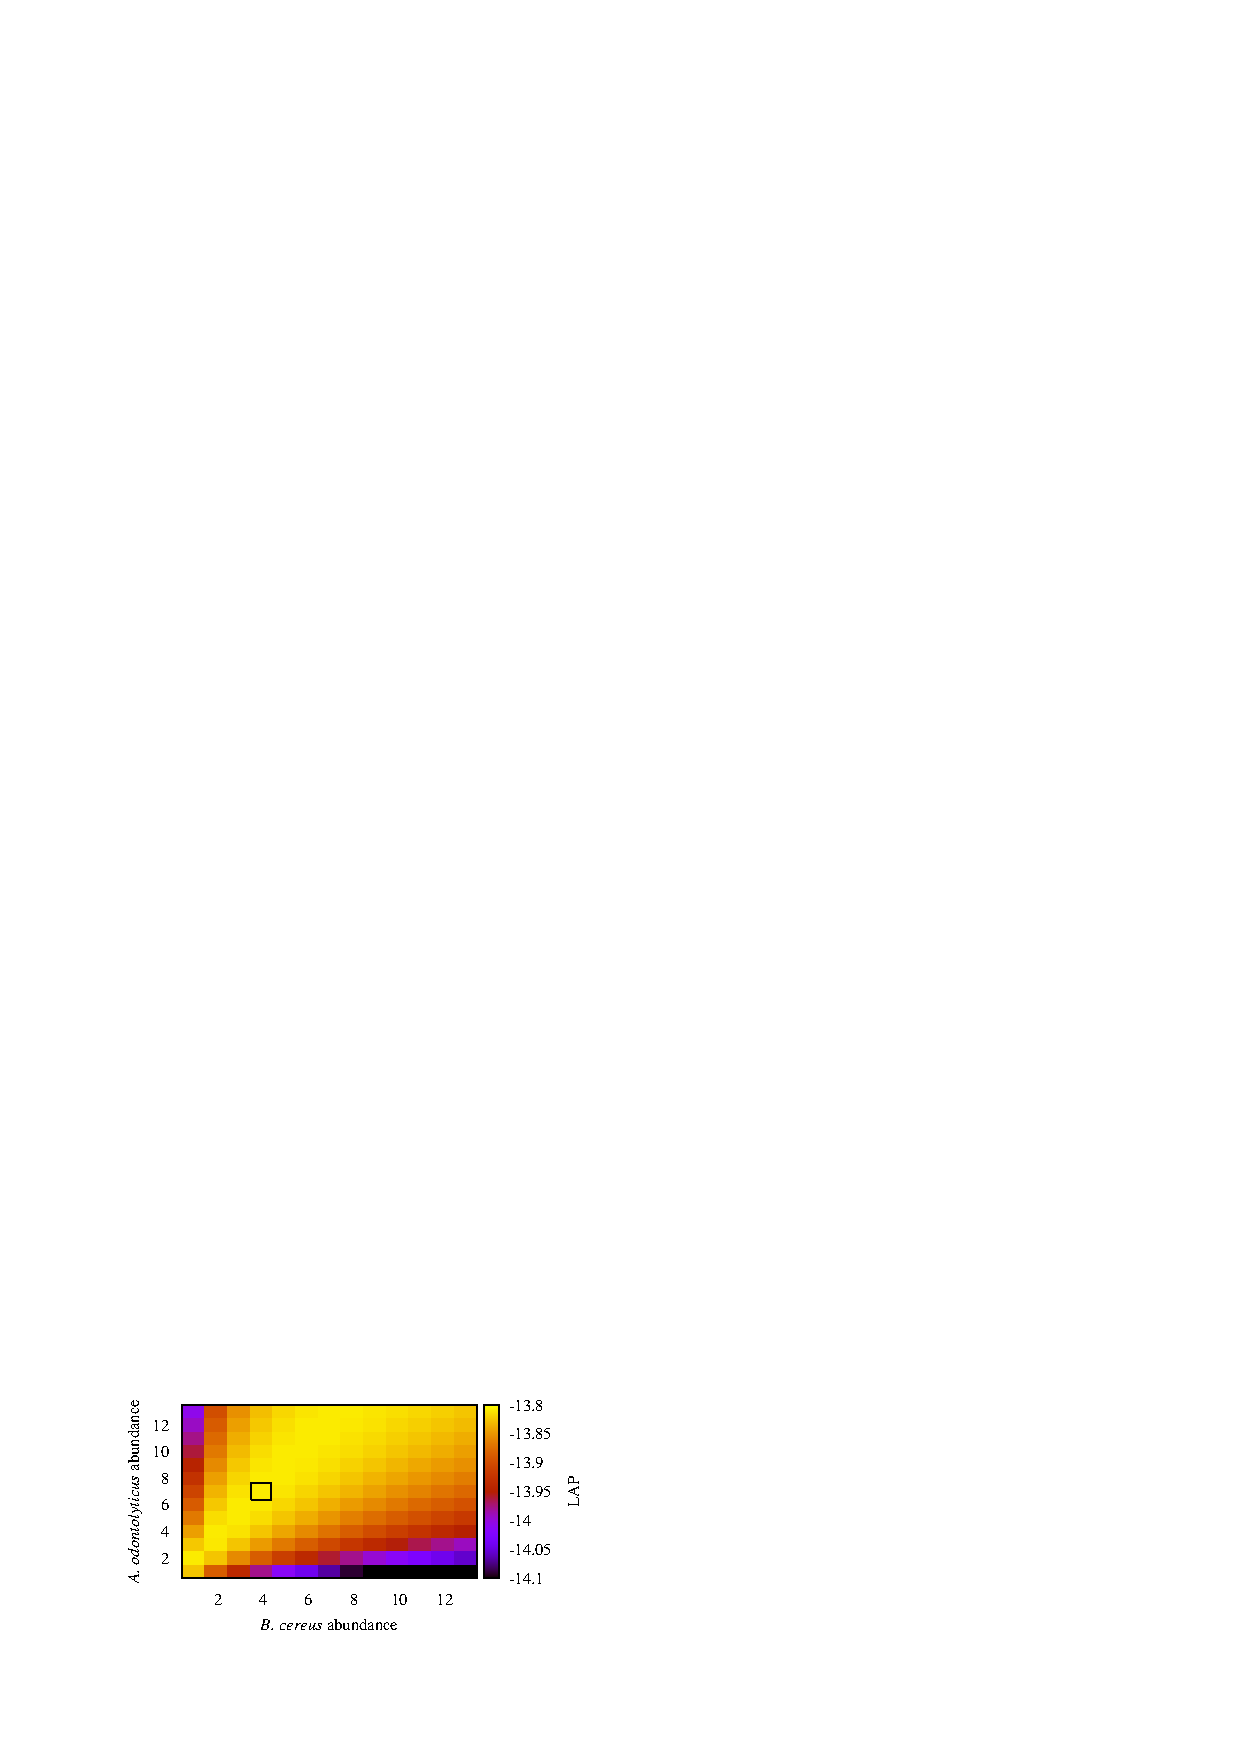
\includegraphics[width=3in]{ref_abun_2}
% where an .eps filename suffix will be assumed under latex,
% and a .pdf suffix will be assumed for pdflatex; or what has been declared
% via \DeclareGraphicsExtensions.
%\caption{LAP scores for simulated B. cereus (4x, 5.2MB) and A. odontolyticus (7x, 2.4MB)}
%\label{fig:ref_abun_2}
%\end{figure}

We expect the highest LAP scores for the assemblies that contain the correct abundance ratios (1:4 or 2:8 in the first community, and 4:7 in the second community).
%1:4 , 2:8 boxes to be highest in figure A, and 4:7, 8:14, etc. in panel 2.  Y
As seen in Figs. \ref{fig:ref_abun_1} and \ref{fig:ref_abun_2}, our LAP score is able to accurately reflect the varying organism abundance ratios present in the sample.
The LAP score increases as the estimates approach the true abundance ratios, with the true ratio yielding the highest LAP scores in both communities.

\begin{figure}[htb!]
\begin{center}
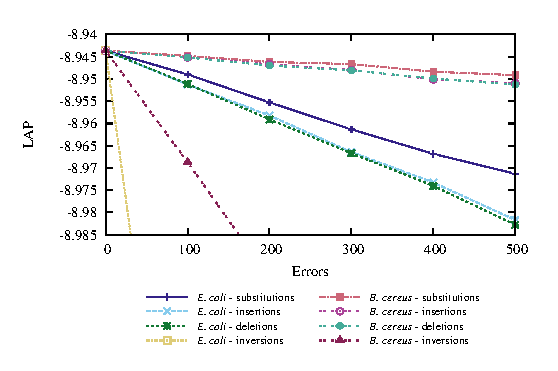
\includegraphics[width=.8\textwidth]{errors}
\end{center}
\renewcommand{\baselinestretch}{1}
\small\normalsize
\begin{quote}
\caption[Synthetic errors in simulated \emph{E. coli} and \emph{B. cereus} (1 copy, 5.2Mbp) community]{Synthetic errors in simulated \emph{E. coli} (5 copies, 4.9Mbp) \emph{B. cereus} (1 copy, 5.2Mbp) community.}
\label{fig:errors}
\end{quote}
\end{figure}
\renewcommand{\baselinestretch}{2}
\small\normalsize

\subsection{Impact of errors on synthetic metagenomes}

One of the often overlooked aspects of metagenomic assembly evaluation is the weighing of errors that occur in contigs with different abundances.
%In single genome assembly, errors are often not weighted since the genome has uniform coverage.
%When detecting errors with the aid of a reference, all substitution errors occurring within a genome are weighted the same (ignoring additional information, such as whether it occurs in a genic or regulatory element).
%When organism abundances are uniform, the weight of an assembly error is also uniform.
In metagenomic samples the relative organism abundances can vary by orders of magnitudes.
A typical reference-based evaluation would equally weight the errors irrespective of the abundance of the erroneous contigs.
The proposed metagenomic LAP score, however, automatically handles this situation and appropriately weighs errors according to genome abundance.
%Thus, errors in highly abundant organisms will have more of an impact on the LAP score than errors in organism of lower abundance.
To illustrate this, we simulated a small metagenomic community consisting of \emph{Escherichia coli} and \emph{Bacillus cereus} at a 5:1 ratio.
We introduced an increasing number of common assembly errors (single-base substitutions, insertions, deletions, and inversions) into the two organisms assemblies and observed the resulting LAP score.

As shown in \figurename~\ref{fig:errors}, the higher the number of synthetic errors, the lower the LAP score.
Insertions/deletions were more deleterious to the LAP score than substitutions, since in addition to causing a mismatch, an insertion/deletion changes the overall genome size.
Although inversions did not change the overall genome size (and would therefore not be detected by simplistic measures such as N50), these errors had the greatest impact on the LAP score because they prevented the alignment of reads across the boundaries of the inversions.
%With substitutions and indels, reads were still able to align across the error and only incurred the additional mismatch penalty.
%Conversely, read alignment tools will fail to detect read alignments that span the borders of the inversions.

%Whereas substitutions, insertions, and deletions still allowed reads to align albeit with a lower probability, reads that inversions are essentially treated as complete

As expected, errors introduced into the more abundant organism, \emph{E. coli}, had a greater affect on the LAP score than those inserted into \emph{B. cereus}.
Our LAP score was able to accurately weigh the errors by the abundance of each organism.


\subsection{Likelihood scores correlate with reference-based metrics}
%c|c|c|c|c|c


With real metagenomic samples, it is difficult to make evaluations given the lack of high quality references.
Using purely simulated data has the issue of not accurately capturing the error and bias introduced by sequencing technology.
Thus, to evaluate our LAP score, we use two `mock' communities (Even and Staggered) provided by the Human Microbiome Project (HMP) consortium\cite{mitreva2012structure,methe2012framework}.
These communities were created using specific DNA sequences from organisms with known reference genomes (consisting of over 20 bacterial genomes and a few eukaryotes) and abundances.
The mock Even community consisted of 100,000 16S copies per organism per aliquot, while the mock Staggered community consisted of 1,000 to 1,000,000 16S copies per organism per aliquot.
Data used from the HMP mock communities are available at \url{http://www.ncbi.nlm.nih.gov/bioproject/48475}.
We calculated the LAP score on assemblies produced by MetAMOS~\cite{treangen2013metamos} using several assemblers: SOAPdenovo~\cite{SOAPdenovo}, Metavelvet~\cite{namiki2012metavelvet}, Velvet~\cite{Velvet}, and Meta-IDBA~\cite{peng2011meta}.
The additional \emph{de novo} and reference-based metrics for the assemblies were taken from MetAMOS~\cite{treangen2013metamos}.  These metrics include:
   \begin{itemize}
   \item number contigs (\# ctgs) -- total number of contigs/scaffolds in the assembly
   \item good contigs (Good Ctgs) -- fraction of contigs that mapped without errors to reference genomes
   \item total aligned (Total aln) -- total amount of sequence (in Mbp) that can be aligned to the reference genomes
   \item slight mis-assemblies (Slt) -- alignments that cover 80\% or more of the aligned contig in a single match (Slt)
   \item heavy misassemblies (Hvy) -- alignments that cover less than 80\% of the aligned contig in a single match or have two or more matches to a single reference
   \item chimeras (Ch) -- contigs with matches to two distinct reference genomes
   \item size at 10 megabases (Size @ 10 Mbp) - the size of the largest contig $c$ such that the sum of all contigs larger than $c$ is more than 10 Mbp (similar to the commonly used N50 size)
   \item max contig size (Max ctg size) -- size of the largest contig in the assembly
   \item errors per megabase (Err per Mbp) -- average number of errors per Mbp in the assembly
   \end{itemize}

Generally, the \emph{de novo} LAP scores agree with the referenced-based metrics (Table \ref{tab:hmp}).
In the mock Even dataset, SOAPdenovo has the greatest LAP score, the highest fraction of contigs that can align to a reference genome without error, total amount of sequence that can be aligned to a reference genome, while also having the lowest amount of misassemblies (including chimeric) and errors per Mbp.
It is important to note that if user selected an assembly based on the best contiguity at 10Mbp, they would select the MetaVelvet assembly, which contains double the error rate per Mbp as the SOAPdenovo assembly while aligning 2Mbp less to the references.

\begin{figure}[tb!]
\begin{center}
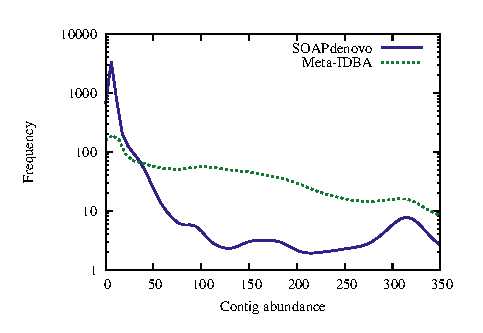
\includegraphics[width=.8\textwidth]{coverage}
\end{center}
\renewcommand{\baselinestretch}{1}
\small\normalsize
\begin{quote}
\caption[Frequency of contig abundances for assemblies of the HMP mock Staggered dataset]{Frequency of contig abundances for assemblies of the HMP mock Staggered dataset.}
\label{fig:coverage}
\end{quote}
\end{figure}
\renewcommand{\baselinestretch}{2}
\small\normalsize


\begin{landscape}
\renewcommand{\baselinestretch}{1}
\small\normalsize

\begin{table}[tbp]
\renewcommand{\arraystretch}{1.2}
\centering
\scriptsize
\begin{tabular}{{l}{l}{c}{c}{c}{c}{c}{c}{c}{c}{c}{c}{c}}
\hline
\bfseries Dataset & \bfseries Assembler & \bfseries LAP & \bfseries \#ctgs &  \bfseries Good ctgs & \bfseries Total aln & \bfseries Slt & \bfseries Hvy & \bfseries Ch & \bfseries Size @ 10 Mbp &\bfseries Max ctg size & \bfseries Err per Mbp & \bfseries Aligned reads \\
\hline\hline

mockE & SOAPdenovo & \textbf{-27.031} & 63107 & \textbf{99.3\%} & \textbf{51} & \textbf{166} & 131          & \textbf{1} & 28,208          & 249,819          & \textbf{5.8}  & \textbf{85.75\%} \\
mockE & Velvet     & -28.537          & 12,830 & 96.2\%          & 41          & 256          & \textbf{100} & 2          & 42,269          & 179,673          & 8.7  & 83.30\%        \\
mockE & MetaVelvet & -27.102          & 22,772 & 96.8\%          & 49          & 462          & 156          & 4          & \textbf{62,138} & \textbf{367,458} & 12.7    & 85.65\%      \\
mockE & Meta-IDBA  & -31.166          & 22,032 & 95.4\%          & 47          & 362          & 151          & 3          & 26,141          & 249,069          & 11  & 81.81\%\\
\\
mockS & SOAPdenovo & -60.161          & 44,928 & \textbf{98.8\%} & \textbf{28} & 135          & 98           & \textbf{0} & 5,672           & 186,064          & \textbf{8.3} & 69.78\%  \\
mockS & Velvet     & -60.711          & 21,050 & 95.8\%          & \textbf{28} & 485          & 115          & 1          & 6,060           & 119,120          & 21.5          & 67.26\% \\
mockS & MetaVelvet & -60.442          & 20,551 & 95.3\%          & \textbf{28} & 517          & 143          & 3          & 6,685           & \textbf{217,330} & 20.1         & 67.72\% \\
mockS & Meta-IDBA  & \textbf{-58.851} & 4,559  & 92.5\%          & 18          & \textbf{101} & \textbf{83}  & \textbf{0} & \textbf{13,150} & 119,604          & 10.2  & \textbf{70.67\%}\\
\\
Tongue  & SOAPdenovo & \textbf{-13.844} & 35,230 & \textbf{89.10\%} & \textbf{11} & 1,138 & 2,618 & \textbf{0} & 11,359 & \textbf{238,051} & \textbf{341.5} & \textbf{88.14\%}\\
Tongue  & Meta-IDBA & -21.368 & 25,698 & 88.70\% & 7 & \textbf{710} & \textbf{2,087} & \textbf{0} & 4,215 & 59,188 & 399.6 & 58.89\% \\

\hline
\end{tabular}
\caption[Comparison of assembly statistics for HMP mock Even and mock Staggered datasets]{Comparison of assembly statistics for HMP mock Even and mock Staggered datasets.Numbers in bold represent the best value for the specific dataset.}
\label{tab:hmp}
\end{table}

\renewcommand{\baselinestretch}{2}
\small\normalsize
\end{landscape}


Since the abundances of each organism in the mock Even dataset are fairly similar, the mock Staggered abundance distribution creates a more realistic scenario encountered in metagenomic environments.
Here, the Meta-IDBA assembly has the greatest LAP score, but aligns roughly a third less sequences to the reference genomes than SOAPdenovo.
The Meta-IDBA assembly contains approximately a tenth of the amount of contigs (4,559 vs. 44,928) as SOAPdenovo.
The SOAPdenovo assembly contains a greater number of contigs at a very low abundance (\figurename~\ref{fig:coverage}).
On large contigs Meta-IDBA performs better than SOAPdenovo and has a lower error rate (see \figurename~4 in \cite{treangen2013metamos}).
However, Meta-IDBA assembles a smaller fraction of the low-abundance genomes than SOAPdenovo, leading fewer sequences to align.
The LAP score penalizes misassemblies within abundant contigs in the SOAPdenovo results.


%Given how the mock Staggered community was constructed (each ratio of 16S copies per aliquot occurred roughly the same number of times), the frequency of contig abundances should be approximately uniform for the community.
%The SOAPdenovo assembly was able to align more reads, but the reads were localized in these low coverage regions.
%The distribution of contig abundances in the Meta-IDBA assembly was closer to the expected distribution than the SOAPdenovo assembly.

%The Meta-IDBA assembly a far more uniform frequency of contig abundances compared to the SOAPdenovo assembly.

Next, we applied our framework on real data where we did not know the actual genomes comprising the sample (HMP tongue dorsum female sample, SRS077736) (Table \ref{tab:hmp}).
Although we do not know for certain which organisms are present in the sample, the HMP identified a reference genome set with high similarity to the sequences within the sample (HMP Shotgun Community profiling SRS077736).
The reference-based error metrics only consider chimeric errors due to the possibility of structural difference between an organism and its version in the reference database.
We calculated the LAP of the assemblies using a single library consisting of 42,013,917 reads.
The SOAPdenovo assembly had a far greater LAP score than the Meta-IDBA assembly.
The higher score is due to the SOAPdenovo assembly recruiting more reads (88.14\% to 58.89\%) in relation to its genome size (46Mbp to 37Mbp) than the Meta-IDBA assembly.
Furthermore, the MetAMOS metrics show that the SOAPdenovo assembly contained approximately 60 less errors per Mbp than the Meta-IDBA assembly.

%These datasets have the advantage over simulated data because it captures the error and bias introduced from the sequence technology.


\renewcommand{\baselinestretch}{1}
\small\normalsize

\begin{table}[tb!]
\label{tab:metamos_lap}
\centering
\begin{tabular}{{l}{c}{c}{c}{c}}
\hline
\bfseries Assembler & \bfseries Contigs & \bfseries LAP & \bfseries N50 (Kbp) & \bfseries  Errors \\
\hline \hline
newbler  & \bf{1} & \bf{-13.064} & \bf{156} & 1 \\
SOAPdenovo & 23 & -14.238 & 9 & \bf{3} \\
Velvet & 3 & -13.157 & 92 & \bf{0} \\
MetaVelvet & 3 & -13.157 & 92 & \bf{0} \\
\hline
\end{tabular}
\caption[Self-tuning MetAMOS using \emph{C. ruddii} test dataset]{Self-tuning MetAMOS using \emph{C. ruddii} test dataset.}
\end{table}

\renewcommand{\baselinestretch}{2}
\small\normalsize

\subsection{Tuning assembly parameters for MetAMOS}
Assemblathon1~\cite{earl2011assemblathon} has shown that assembly experts can often get drastically different assemblies using the same assemblers, highlighting the difficulty of choosing the \emph{right} parameters for a given assembler.
Our metagenomic LAP framework comes packaged with the MetAMOS pipeline, allowing users the option to run MetAMOS with different assemblers and automatically select the assembly with the highest LAP score.
This step occurs without any prior knowledge from the user.

We showcase the ease of use of the automated assembler selection within MetAMOS using the \emph{Carsonella ruddii} (156Kbp) dataset packaged with MetAMOS (Table ~\ref{tab:metamos_lap}).
Errors were found using DNADIFF~\cite{phillippy2008genome} and MUMmer~\cite{delcher2003using}.
The newbler assembly produced one contig containing the complete \emph{C. ruddii} genome.
The SOAPdenovo assembly produced a severely fragmented assembly with the most number of errors.
The MetaVelvet and Velvet produced identical assemblies, containing 3 contigs of sizes 92Kbp, 65Kbp, and 1.7Kbp, but contained an additional 158bp compared to the \emph{C. ruddii} genome.
Upon closer inspection, there were overlaps between the contigs ranging from 38bp to 73bp.
This is not surprising given MetaVelvet's and Velvet's de bruijn graph-based approach could not resolve repetitive regions between the contigs.
Newbler, on the other hand, contained only a single insertion error.
The LAP score of the Newbler assembly was greater due to more reads being able to align across the regions that were broken apart in the MetaVelvet and Velvet assemblies.
Additionally, the Newbler assembly did not contain the duplicated sequence found in the other assemblies.
MetAMOS was able to select the most likely assembly without requiring any additional input from the user.

\section{Discussion}

In this chapter, we have proposed an extension to our LAP framework to perform \emph{de novo} comparisons of metagenomic assemblies.
Unlike traditional \emph{de novo} metrics used for measuring assembly quality, our extended LAP score correlates well with reference-based measures of metagenomic assembly quality.
However, in this study, we have realized that there is a lack of reference-based metrics when evaluating metagenomic assemblies.
Misjoins betweens organisms may be more deleterious than misjoins within a single genome.
Furthermore, current reference-based metrics do not take into account the relative abundances of the organisms when evaluating metagenomic assemblies.
The metrics provided by MetAMOS do not factor in the contig abundances when examining assembly errors.
This made it difficult to compare our LAP score to their reference-based metrics because, intuitively, an error in a highly abundant organism should be \emph{worse} than an error in a rare, low coverage organism.
Our LAP score implicitly weighs the errors in abundant contigs more than those in lesser abundant contigs.
In our results, we have proposed one such reference-based metric that scales the errors by the relative abundance of the contig it occurs within.

It is important to note that we have only focused on the complete reconstruction of the metagenome from the set of reads.
Assembly algorithms are designed with specific biological applications in mind, such as, the conservative reconstruction of the genic regions.
Studies focusing on the genic regions may tolerate large-scale rearrangements as long as the genic regions were correctly assembled.
Conversely, other studies may want to focus on the reconstruction and detection of rare pathogenic bacteria in an environment.
These application specific assembly algorithms all attempt to optimize their formulation of the assembly problem.

Our metagenomic LAP extension relies heavily on the idea that the sequencing process of the metagenome is roughly uniform, and that the reads are independently sampled from the genome.
Biases exist in all steps of the sequencing process, from the extraction of DNA from organisms with different cell membranes/walls~\cite{carrigg2007dna,krsek1999comparison} to the sequencing protocol used~\cite{morgan2010metagenomic,temperton2009bias}.
In the future, we would like to implement a more specific model that better captures the sequencing process.

%De novo metric, more misleading in assemblies -> chimera

%We would like to stress that \emph{de novo} measures of assembly quality, such as ours, are critically needed by researchers attempting to assemble of yet unknown genomes.

Results from GAGE~\cite{salzberg2011gage} and Assemblathon~\cite{earl2011assemblathon,bradnam2013assemblathon} have shown that the specific characteristics of the data being assembled has a great impact on the performance of the assembler.
This problem is magnified in metagenomic assembly.
By integrating our LAP framework in MetAMOS, we have allowed researchers to accurately and effortlessly run and evaluate assemblies without any prior knowledge on evaluating assembly quality.

In our framework, we use the average coverage of the contig (provided by MetAMOS) to estimate abundance.
There are issues with this measure as it is possible that mis-assembled repeats within a contig will affect our estimate of depth of coverage and could impact our underlying statistics.
A better approach is to use something more robust than the mean coverage, such as the median coverage, to avoid being influenced by such regions.
While the user can supply the median coverage to our standalone framework, future work includes building this feature into MetAMOS.
Another approach involves breaking contigs at regions of differing coverage (using tools such as AMOSvalidate\cite{phillippy2008genome}), so there will be less deviation in the average coverage within the contig.

It should be noted that in some cases it may not be tractable to run the complete collection of assemblers with MetAMOS.
In such cases, we should first employ heuristics (such as \cite{chikhi2013informed}) to aid in selecting potential assemblers (and parameters) to run.
For the assembler selection process, we can use the LAP framework's sampling procedure in combination with calculating read probabilities in parallel to reduce runtime.

Our goal was to provide a global measure of how good a metagenomic assembly may be, not to detect assembly errors.
Other likelihood-based frameworks, such as ALE, use frequencies of certain sequences to aid in detection of possible chimeric contigs.
We are able to apply similar modifications to our LAP framework to find regions of possible misassembly.
Finally, we plan to extend our framework to give a more detailed breakdown of the LAP scores of segments assembled using the same subset of reads across different assemblies.
The goal would be to take high-scoring assembled segments from individual assemblies to recreate an assembly with overall greater likelihood.
This approach will be of great benefit to the field of metagenomic assembly since assemblers are often designed with different constraints and goals in mind, e.g., low memory footprint, assembling high/low coverage organisms, or tolerating population polymorphisms.
For example, on the mock Staggered dataset, Meta-IDBA best assembled the most abundant genomes while SOAPdenovo had a better representation of the low abundance organisms.
Providing a systematic way of combining assembler approaches using our LAP score will produce better assemblies for downstream analyses.


% An example of a floating figure using the graphicx package.
% Note that \label must occur AFTER (or within) \caption.
% For figures, \caption should occur after the \includegraphics.
% Note that IEEEtran v1.7 and later has special internal code that
% is designed to preserve the operation of \label within \caption
% even when the captionsoff option is in effect. However, because
% of issues like this, it may be the safest practice to put all your
% \label just after \caption rather than within \caption{}.
%
% Reminder: the "draftcls" or "draftclsnofoot", not "draft", class
% option should be used if it is desired that the figures are to be
% displayed while in draft mode.
%
%\begin{figure}[!t]
%\centering
%\includegraphics[width=2.5in]{myfigure}
% where an .eps filename suffix will be assumed under latex,
% and a .pdf suffix will be assumed for pdflatex; or what has been declared
% via \DeclareGraphicsExtensions.
%\caption{Simulation Results}
%\label{fig_sim}
%\end{figure}

% Note that IEEE typically puts floats only at the top, even when this
% results in a large percentage of a column being occupied by floats.


% An example of a double column floating figure using two subfigures.
% (The subfig.sty package must be loaded for this to work.)
% The subfigure \label commands are set within each subfloat command, the
% \label for the overall figure must come after \caption.
% \hfil must be used as a separator to get equal spacing.
% The subfigure.sty package works much the same way, except \subfigure is
% used instead of \subfloat.
%
%\begin{figure*}[!t]
%\centerline{\subfloat[Case I]\includegraphics[width=2.5in]{subfigcase1}%
%\label{fig_first_case}}
%\hfil
%\subfloat[Case II]{\includegraphics[width=2.5in]{subfigcase2}%
%\label{fig_second_case}}}
%\caption{Simulation results}
%\label{fig_sim}
%\end{figure*}
%
% Note that often IEEE papers with subfigures do not employ subfigure
% captions (using the optional argument to \subfloat), but instead will
% reference/describe all of them (a), (b), etc., within the main caption.


% An example of a floating table. Note that, for IEEE style tables, the
% \caption command should come BEFORE the table. Table text will default to
% \footnotesize as IEEE normally uses this smaller font for tables.
% The \label must come after \caption as always.
%
%\begin{table}[!t]
%% increase table row spacing, adjust to taste
%\renewcommand{\arraystretch}{1.3}
% if using array.sty, it might be a good idea to tweak the value of
% \extrarowheight as needed to properly center the text within the cells
%\caption{An Example of a Table}
%\label{table_example}
%\centering
%% Some packages, such as MDW tools, offer better commands for making tables
%% than the plain LaTeX2e tabular which is used here.
%\begin{tabular}{|c||c|}
%\hline
%One & Two\\
%\hline
%Three & Four\\
%\hline
%\end{tabular}
%\end{table}


% Note that IEEE does not put floats in the very first column - or typically
% anywhere on the first page for that matter. Also, in-text middle ("here")
% positioning is not used. Most IEEE journals/conferences use top floats
% exclusively. Note that, LaTeX2e, unlike IEEE journals/conferences, places
% footnotes above bottom floats. This can be corrected via the \fnbelowfloat
% command of the stfloats package.



\section{Conclusion}
In this chapter we have described an extension to our \emph{de novo} assembly evaluation framework (LAP) for comparing metagenomic assemblies.
We showed that the true metagenome and correct relative abundances maximizes our extended LAP score.
Furthermore, we have integrated our framework into the metagenomic assembly pipeline MetAMOS, showing that any user is able to reproduce quality evaluations of metagenomic assemblies with relative ease.

%%%
%% This is file `supertabular.sty',
%% generated with the docstrip utility.
%%
%% The original source files were:
%%
%% supertabular.dtx  (with options: `package')
%% Copyright (C) 1989-2004 Johannes Braams. All rights reserved.
%% 
%% This file was generated from file(s) of the supertabular package.
%% -----------------------------------------------------------------
%% 
%% It may be distributed and/or modified under the
%% conditions of the LaTeX Project Public License, either version 1.3
%% of this license or (at your option) any later version.
%% The latest version of this license is in
%%   http://www.latex-project.org/lppl.txt
%% and version 1.3 or later is part of all distributions of LaTeX
%% version 2003/12/01 or later.
%% 
%% This work has the LPPL maintenance status "maintained".
%% 
%% The Current Maintainer of this work is Johannes Braams.
%% 
%% This file may only be distributed together with a copy of the
%% supertabular package. You may however distribute the supertabular package
%% without such generated files.
%% 
%% The list of all files belonging to the supertabular package is
%% given in the file `manifest.txt.
%% 
%% The list of derived (unpacked) files belonging to the distribution
%% and covered by LPPL is defined by the unpacking scripts (with
%% extension .ins) which are part of the distribution.
%% Sourcefile `supertabular.dtx'.
%%
%% Copyright (C) 1988 by Theo Jurriens
%% Copyright (C) 1990-2004 by Johannes Braams texniek at braams.cistron.nl
%%                            Kersengaarde 33
%%                            2723 BP Zoetermeer NL
%%                       all rights reserved.
%%
%%
\NeedsTeXFormat{LaTeX2e}
\ProvidesPackage{supertabular}
              [2004/02/20 v4.1e the supertabular environment]
\newcount\c@tracingst
\DeclareOption{errorshow}{\c@tracingst\z@}
\DeclareOption{pageshow}{\c@tracingst\tw@}
\DeclareOption{debugshow}{\c@tracingst5\relax}
\ProcessOptions
\newif\if@topcaption \@topcaptiontrue
\def\topcaption{\@topcaptiontrue\tablecaption}
\def\bottomcaption{\@topcaptionfalse\tablecaption}
\long\def\tablecaption{%
  \refstepcounter{table}\@dblarg{\@xtablecaption}}
\long\def\@xtablecaption[#1]#2{%
  \long\gdef\@process@tablecaption{\ST@caption{table}[#1]{#2}}}
\global\let\@process@tablecaption\relax
\newif\ifST@star
\newif\ifST@mp
\newdimen\ST@wd
\newskip\ST@rightskip
\newskip\ST@leftskip
\newskip\ST@parfillskip
\long\def\ST@caption#1[#2]#3{\par%
  \addcontentsline{\csname ext@#1\endcsname}{#1}%
                  {\protect\numberline{%
                      \csname the#1\endcsname}{\ignorespaces #2}}
  \begingroup
    \@parboxrestore
    \normalsize
    \if@topcaption \vskip -10\p@ \fi
    \@makecaption{\csname fnum@#1\endcsname}{\ignorespaces #3}\par
    \if@topcaption \vskip 10\p@ \fi
  \endgroup}
\newcommand\tablehead[1]{%
  \gdef\@tablehead{%
  \noalign{%
      \global\let\@savcr=\\
      \global\let\\=\org@tabularcr}%
    #1%
    \noalign{\global\let\\=\@savcr}}}
\tablehead{}
\newcommand\tablefirsthead[1]{\gdef\@table@first@head{#1}}
\newcommand\tabletail[1]{%
  \gdef\@tabletail{%
    \noalign{%
      \global\let\@savcr=\\
      \global\let\\=\org@tabularcr}%
    #1%
    \noalign{\global\let\\=\@savcr}}}
\tabletail{}
\newcommand\tablelasttail[1]{\gdef\@table@last@tail{#1}}
\newcommand\sttraceon{\c@tracingst5\relax}
\newcommand\sttraceoff{\c@tracingst\z@}
\newcommand\ST@trace[2]{%
  \ifnum\c@tracingst>#1\relax
    \GenericWarning
      {(supertabular)\@spaces\@spaces}
      {Package supertabular: #2}%
  \fi
  }
\newdimen\ST@pageleft
\newcommand*\shrinkheight[1]{%
  \noalign{\global\advance\ST@pageleft-#1\relax}}
\newcommand*\setSTheight[1]{%
  \noalign{\global\ST@pageleft=#1\relax}}
\newdimen\ST@headht
\newdimen\ST@tailht
\newdimen\ST@pagesofar
\newdimen\ST@pboxht
\newdimen\ST@lineht
\newdimen\ST@stretchht
\newdimen\ST@prevht
\newdimen\ST@toadd
\newdimen\ST@dimen
\newbox\ST@pbox
\def\ST@tabularcr{%
  {\ifnum0=`}\fi
  \@ifstar{\ST@xtabularcr}{\ST@xtabularcr}}
\def\ST@xtabularcr{%
  \@ifnextchar[%]
    {\ST@argtabularcr}%
    {\ifnum0=`{\fi}\cr\ST@cr}}
\def\ST@argtabularcr[#1]{%
  \ifnum0=`{\fi}%
  \ifdim #1>\z@
    \unskip\ST@xargarraycr{#1}
  \else
    \ST@yargarraycr{#1}%
  \fi}
\def\ST@xargarraycr#1{%
  \@tempdima #1\advance\@tempdima \dp \@arstrutbox
  \vrule \@height\z@ \@depth\@tempdima \@width\z@ \cr
  \noalign{\global\ST@toadd=#1}\ST@cr}
\def\ST@yargarraycr#1{%
  \cr\noalign{\vskip #1\global\ST@toadd=#1}\ST@cr}
\def\ST@startpbox#1{%
  \setbox\ST@pbox\vtop\bgroup\hsize#1\@arrayparboxrestore}
\def\ST@astartpbox#1{%
  \bgroup\hsize#1%
  \setbox\ST@pbox\vtop\bgroup\hsize#1\@arrayparboxrestore}
\def\ST@endpbox{%
  \@finalstrut\@arstrutbox\par\egroup
  \ST@dimen=\ht\ST@pbox
  \advance\ST@dimen by \dp\ST@pbox
  \ifnum\ST@pboxht<\ST@dimen
    \global\ST@pboxht=\ST@dimen
  \fi
  \ST@dimen=\z@
  \box\ST@pbox\hfil}
\def\ST@aendpbox{%
  \@finalstrut\@arstrutbox\par\egroup
  \ST@dimen=\ht\ST@pbox
  \advance\ST@dimen by \dp\ST@pbox
  \ifnum\ST@pboxht<\ST@dimen
    \global\ST@pboxht=\ST@dimen
  \fi
  \ST@dimen=\z@
  \unvbox\ST@pbox\egroup\hfil}
\def\estimate@lineht{%
  \ST@lineht=\arraystretch \baslineskp
  \global\advance\ST@lineht by 1\p@
  \ST@stretchht\ST@lineht\advance\ST@stretchht-\baslineskp
  \ifdim\ST@stretchht<\z@\ST@stretchht\z@\fi
  \ST@trace\tw@{Average line height: \the\ST@lineht}%
  \ST@trace\tw@{Stretched line height: \the\ST@stretchht}%
  }
\def\@calfirstpageht{%
  \ST@trace\tw@{Calculating height of tabular on first page}%
  \global\ST@pagesofar\pagetotal
  \global\ST@pageleft\@colroom
  \ST@trace\tw@{Height of text = \the\pagetotal; \MessageBreak
                Height of page = \the\ST@pageleft}%
  \if@twocolumn
    \ST@trace\tw@{two column mode}%
    \if@firstcolumn
     \ST@trace\tw@{First column}%
      \ifnum\ST@pagesofar > \ST@pageleft
        \global\ST@pageleft=2\ST@pageleft
        \ifnum\ST@pagesofar > \ST@pageleft
          \newpage\@calnextpageht
          \ST@trace\tw@{starting new page}%
        \else
          \ST@trace\tw@{Second column}%
          \global\advance\ST@pageleft -\ST@pagesofar
          \global\advance\ST@pageleft -\@colroom
        \fi
      \else
        \global\advance\ST@pageleft by -\ST@pagesofar
        \global\ST@pagesofar\z@
      \fi
    \else
      \ST@trace\tw@{Second column}
      \ifnum\ST@pagesofar > \ST@pageleft
        \ST@trace\tw@{starting new page}%
        \newpage\@calnextpageht
      \else
        \global\advance\ST@pageleft by -\ST@pagesofar
        \global\ST@pagesofar\z@
      \fi
    \fi
  \else
    \ST@trace\tw@{one column mode}%
    \ifnum\ST@pagesofar > \ST@pageleft
      \ST@trace\tw@{starting new page}%
      \newpage\@calnextpageht
    \else
      \global\advance\ST@pageleft by -\ST@pagesofar
      \global\ST@pagesofar\z@
    \fi
  \fi
  \ST@trace\tw@{Available height: \the\ST@pageleft}%
  \ifx\@@tablehead\@empty
    \ST@headht=\z@
  \else
    \setbox\@tempboxa=\vbox{\@arrayparboxrestore
      \ST@restore
      \expandafter\tabular\expandafter{\ST@tableformat}%
      \@@tablehead\endtabular}%
    \ST@headht=\ht\@tempboxa\advance\ST@headht\dp\@tempboxa
  \fi
  \ST@trace\tw@{Height of head: \the\ST@headht}%
  \ifx\@tabletail\@empty
    \ST@tailht=\z@
  \else
    \setbox\@tempboxa=\vbox{\@arrayparboxrestore
      \ST@restore
      \expandafter\tabular\expandafter{\ST@tableformat}
        \@tabletail\endtabular}
    \ST@tailht=\ht\@tempboxa\advance\ST@tailht\dp\@tempboxa
  \fi
  \advance\ST@tailht by \ST@lineht
  \ST@trace\tw@{Height of tail: \the\ST@tailht}%
  \ST@trace\tw@{Maximum height of tabular: \the\ST@pageleft}%
  \@tempdima\ST@headht
  \advance\@tempdima\ST@lineht
  \advance\@tempdima\ST@tailht
  \ST@trace\tw@{Minimum height of tabular: \the\@tempdima}%
  \ifnum\@tempdima>\ST@pageleft
    \ST@trace\tw@{starting new page}%
    \newpage\@calnextpageht
  \fi
}
\def\@calnextpageht{%
  \ST@trace\tw@{Calculating height of tabular on next page}%
  \global\ST@pageleft\@colroom
  \global\ST@pagesofar=\z@
  \ST@trace\tw@{Maximum height of tabular: \the\ST@pageleft}%
  }
\def\x@supertabular{%
  \let\org@tabular\tabular
  \let\tabular\inner@tabular
  \expandafter\let
    \csname org@tabular*\expandafter\endcsname
    \csname tabular*\endcsname
  \expandafter\let\csname tabular*\expandafter\endcsname
    \csname inner@tabular*\endcsname
  \if@topcaption \@process@tablecaption \fi
  \global\let\@oldcr=\\
  \def\baslineskp{\baselineskip}%
  \ifx\undefined\@classix
    \let\org@tabularcr\@tabularcr
    \let\@tabularcr\ST@tabularcr
    \let\org@startpbox=\@startpbox
    \let\org@endpbox=\@endpbox
    \let\@@startpbox=\ST@startpbox
    \let\@@endpbox=\ST@endpbox
  \else
    \let\org@tabularcr\@arraycr
    \let\@arraycr\ST@tabularcr
    \let\org@startpbox=\@startpbox
    \let\org@endpbox=\@endpbox
    \let\@startpbox=\ST@astartpbox
    \let\@endpbox=\ST@aendpbox
  \fi
  \ifx\@table@first@head\undefined
    \let\@@tablehead=\@tablehead
  \else
    \let\@@tablehead=\@table@first@head
  \fi
  \let\ST@skippage\ST@skipfirstpart
  \estimate@lineht
  \@calfirstpageht
  \noindent
  }
\def\supertabular{%
  \@ifnextchar[{\@supertabular}%]
               {\@supertabular[]}}
\def\@supertabular[#1]#2{%
  \def\ST@tableformat{#2}%
  \ST@trace\tw@{Starting a new supertabular}%
  \global\ST@starfalse
  \global\ST@mpfalse
  \x@supertabular
  \expandafter\org@tabular\expandafter{\ST@tableformat}%
  \@@tablehead}
\@namedef{supertabular*}#1{%
  \@ifnextchar[{\@nameuse{@supertabular*}{#1}}%
               {\@nameuse{@supertabular*}{#1}[]}%]
  }
\@namedef{@supertabular*}#1[#2]#3{%
  \ST@trace\tw@{Starting a new supertabular*}%
  \def\ST@tableformat{#3}%
  \ST@wd=#1\relax
  \global\ST@startrue
  \global\ST@mpfalse
  \x@supertabular
  \expandafter\csname org@tabular*\expandafter\endcsname
  \expandafter{\expandafter\ST@wd\expandafter}%
  \expandafter{\ST@tableformat}%
  \@@tablehead}%
\def\mpsupertabular{%
  \@ifnextchar[{\@mpsupertabular}%]
               {\@mpsupertabular[]}}
\def\@mpsupertabular[#1]#2{%
  \def\ST@tableformat{#2}%
  \ST@trace\tw@{Starting a new mpsupertabular}%
  \global\ST@starfalse
  \global\ST@mptrue
  \ST@rightskip \rightskip
  \ST@leftskip \leftskip
  \ST@parfillskip \parfillskip
  \x@supertabular
  \minipage{\columnwidth}%
  \parfillskip\ST@parfillskip
  \rightskip \ST@rightskip
  \leftskip \ST@leftskip
  \noindent\expandafter\org@tabular\expandafter{\ST@tableformat}%
  \@@tablehead}
\@namedef{mpsupertabular*}#1{%
  \@ifnextchar[{\@nameuse{@mpsupertabular*}{#1}}%
               {\@nameuse{@mpsupertabular*}{#1}[]}%]
  }
\@namedef{@mpsupertabular*}#1[#2]#3{%
  \ST@trace\tw@{Starting a new mpsupertabular*}%
  \def\ST@tableformat{#3}%
  \ST@wd=#1\relax
  \global\ST@startrue
  \global\ST@mptrue
  \ST@rightskip \rightskip
  \ST@leftskip \leftskip
  \ST@parfillskip \parfillskip
  \x@supertabular
  \minipage{\columnwidth}%
  \parfillskip\ST@parfillskip
  \rightskip \ST@rightskip
  \leftskip \ST@leftskip
  \noindent\expandafter\csname org@tabular*\expandafter\endcsname
  \expandafter{\expandafter\ST@wd\expandafter}%
  \expandafter{\ST@tableformat}%
  \@@tablehead}%
\def\endsupertabular{%
  \ifx\@table@last@tail\undefined
    \@tabletail
  \else
    \@table@last@tail
  \fi
  \csname endtabular\ifST@star*\fi\endcsname
  \ST@restore
  \if@topcaption
  \else
    \@process@tablecaption
    \@topcaptiontrue
  \fi
  \global\let\\\@oldcr
  \global\let\@process@tablecaption\relax
  \ST@trace\tw@{Ended a supertabular\ifST@star*\fi}%
  }
\expandafter\let\csname endsupertabular*\endcsname\endsupertabular
\def\endmpsupertabular{%
  \ifx\@table@last@tail\undefined
    \@tabletail
  \else
    \@table@last@tail
  \fi
  \csname endtabular\ifST@star*\fi\endcsname
  \endminipage
  \ST@restore
  \if@topcaption
  \else
    \@process@tablecaption
    \@topcaptiontrue
  \fi
  \global\let\\\@oldcr
  \global\let\@process@tablecaption\relax
  \ST@trace\tw@{Ended a mpsupertabular\ifST@star*\fi}%
  }
\expandafter\let\csname endmpsupertabular*\endcsname\endmpsupertabular
\def\ST@restore{%
  \ifx\undefined\@classix
    \let\@tabularcr\org@tabularcr
  \else
    \let\@arraycr\org@tabularcr
  \fi
  \let\@startpbox\org@startpbox
  \let\@endpbox\org@endpbox
  }
\def\inner@tabular{%
  \ST@restore
  \let\\\@oldcr
  \noindent
  \org@tabular}
\@namedef{inner@tabular*}{%
  \ST@restore
  \let\\\@oldcr
  \noindent
  \csname org@tabular*\endcsname}
\def\ST@cr{%
  \noalign{%
    \ifnum\ST@pboxht<\ST@lineht
      \global\advance\ST@pageleft -\ST@lineht
      \global\ST@prevht\ST@lineht
    \else
     \ST@trace\thr@@{Added par box with height \the\ST@pboxht}%
      \global\advance\ST@pageleft -\ST@pboxht
      \global\advance\ST@pageleft -0.1\ST@pboxht
      \global\advance\ST@pageleft -\ST@stretchht
      \global\ST@prevht\ST@pboxht
      \global\ST@pboxht\z@
    \fi
    \global\advance\ST@pageleft -\ST@toadd
    \global\ST@toadd=\z@
    \ST@trace\thr@@{Space left for tabular: \the\ST@pageleft}%
  }
  \noalign{\global\let\ST@next\@empty}%
  \ifnum\ST@pageleft<\z@
    \ST@skippage
  \else
    \noalign{\global\@tempdima\ST@tailht
      \global\advance\@tempdima\ST@prevht
    \ifST@mp
      \ifvoid\@mpfootins\else
        \global\advance\@tempdima\ht\@mpfootins
        \global\advance\@tempdima 3pt
      \fi
    \fi}
    \ifnum\ST@pageleft<\@tempdima
      \ST@newpage
    \fi
  \fi
  \ST@next}
\def\ST@skipfirstpart{%
  \noalign{%
    \ST@trace\tw@{Tabular too high, moving to next page}%
    \global\advance\ST@pageleft\pagetotal
    \global\ST@pagesofar\z@
    \newpage
    \global\let\ST@skippage\ST@newpage
    }}
\def\ST@newpage{%
  \noalign{\ST@trace\tw@{Starting new page, writing tail}}%
  \@tabletail
  \ifST@star
    \csname endtabular*\endcsname
  \else
    \endtabular
  \fi
  \ifST@mp
    \endminipage
  \fi
  \global\let\ST@skippage\ST@newpage
  \newpage\@calnextpageht
  \let\ST@next\@tablehead
  \ST@trace\tw@{writing head}%
  \ifST@mp
    \noindent\minipage{\columnwidth}%
    \parfillskip\ST@parfillskip
    \rightskip \ST@rightskip
    \leftskip \ST@leftskip
  \fi
  \noindent
  \ifST@star
    \expandafter\csname org@tabular*\expandafter\endcsname
    \expandafter{\expandafter\ST@wd\expandafter}%
    \expandafter{\ST@tableformat}%
  \else
    \expandafter\org@tabular\expandafter{\ST@tableformat}%
  \fi}
\endinput
%%
%% End of file `supertabular.sty'.

\titleformat{\chapter}
      {\normalfont\large}{Appendix \thechapter:}{1em}{}
%%Appendix -- January 2015
\appendix
\renewcommand{\thechapter}{A}
\renewcommand{\chaptername}{Appendix}

\chapter{Previous Experiments}

The understanding of nonlinear processes in optical fibers is crucial towards 
extending the capabilities of modern optical communication systems based on 
wavelength division multiplexing (WDM), where each communication channel is 
represented by a unique wavelength. One of the nonlinear processes that 
limits the information carrying capacity of a WDM system is four-wave mixing 
(FWM), which causes cross-talk between neighboring channels. This places a 
lower limit on the wavelength separation between adjacent channels and an
upper limit on the input power in each channel. In this study, we describe
a process by which the evolution of FWM processes in an optical fiber can be 
used to estimate the inhomogeneities in the fiber core material, in particular 
the fluctuations in the linear refractive index of the fiber core.  

\section{Overview}

Experiments measuring the evolution of FWM processes along a length of fiber 
were carried out by Hart {\it et al.}\ \cite{hart1} and are described in detail in 
Sec.\ 2.2. In this experiment, two input pump waves at frequencies
$\omega_1$ and $\omega_2$, interacted with each other through the third-order 
nonlinearity of the fiber material to generate first-order sidebands at frequencies 
$\omega_3 = 2\omega_1 - \omega_2$ and $\omega_4 = 2\omega_2 - \omega_1$. 
These waves further interacted to produce second-order sidebands at 
$\omega_5 = 2\omega_3 - \omega_4$ and $\omega_6 = 2\omega_4 - \omega_3$. 
Higher-order sidebands were also generated. The normalized power in the 
sideband at frequency $\omega_m$ was represented by $\rho_m$. The 
evolution of the FWM processes was characterized by the evolution of 
$\rho_m$(z) as a function of fiber length z. 

In the present work, we make a quantitative comparison between these 
experimental results and our numerical results based on efficient algorithms 
\cite{Agrawal2} to solve the nonlinear Schr\"odinger equation (NLSE) that
governs the system. The numerical model, its underlying assumptions and
the results are described in Sec.\ 2.3. A realistic description of a 
standard single mode optical fiber must take into account the random phase 
perturbations a light wave undergoes while propagating through it, without 
disturbing the underlying conservative properties of the system. The NLSE 
needs to be suitably modified in order to incorporate the stochastic nature 
of the propagation. In order to preserve the conservative properties of the 
system, the stochastic terms in the NLSE must necessarily be multiplicative in 
nature as an additive term acts as a source or a sink. An algorithm that 
achieves this with linear, Gaussian, $\delta$-correlated noise is outlined in 
Sec.\ 2.3. This algorithm preserves the unconditional stability of the 
system. At the same time, care is taken to transform the stochastic NLSE from 
its original Ito representation \cite{ito} to the computationally feasible Stratanovich 
representation \cite{stratanovich} by compensating for the 
spurious linear drift that results from integrating such stochastic 
differential equations \cite{risken,werner2,drummond1,carter3}. The dominant 
sources of phase noise are discussed in Sec.\ 2.4. 

Conclusions on the relevance of the experiments of Hart {\it et al.}\ \cite{hart1} 
and the stochastic modeling presented here are summarized in Sec.\ 2.5.    

\section{Experimental and Computational Background}

In this work, we focus on tracing the evolution of the sidebands, generated 
through FWM, along a length of optical fiber. The FWM spectral evolution along
50\,m of fiber for two input pump power regimes (2.1\,W and 5.5\,W) was
investigated \cite{hart1}. In the 2.1\,W case, the sideband evolution followed a damped 
sinusoid along the length of the fiber. The experiments also found that the 
two first-order sidebands ($\rho_3$-blueshifted and $\rho_4$-redshifted from 
the two pumps) had different evolutions along the fiber (with different 
spatial wavelengths). For the 5.5\,W case, the evolution of both first- and 
second-order sidebands was measured. The damping in the first-order sidebands 
($\rho_3$ and $\rho_4$) occured faster than in the 2.1\,W case. Experiments 
probing the dependence of the sideband power on the input power (ranging from 
2\,W to 17\,W) were also performed at a fixed output length of 50\,m of the fiber.
At the same fiber length, the optical spectra for input powers ranging from 
2\,W to 17\,W were also recorded \cite{hart1}. The spectral envelopes were observed to fit 
well to a hyperbolic secant function and the fit parameters were recorded. 
Measurements with a high-resolution wavemeter showed that one of the two pumps 
consisted of two very closely spaced longitudinal modes 
($\Delta\nu\sim$ 0.5\,GHz) which were not resolved by the spectrometer used to 
record the FWM spectra. Inclusion of this multimode nature of the pump input 
in their model was found to alter the sideband dynamics dramatically and 
partly explained the asymmetry between the blue-shifted and red-shifted 
sidebands though it did not account for the damping in the sidebands. This 
was accounted for by adding weak phase fluctuations to the waves as they 
propagated along the fiber \cite{hart1}. The physical source of these phase fluctuations 
was not known at that time. However, the inclusion of the phase fluctuations 
into the model gave excellent qualitative and quantitative agreement with 
experiment. Their model involved integration of a system of coupled ODEs 
derived from the NLSE \cite{thompson1} by a process of truncation that 
retained only the leading frequency components (the pumps and the first- and 
second-order sidebands), a process justified by the fact that the input pump 
waves are well approximated by a combination of monochromatic waves. Their 
final numerical results are based on simulations using the truncated-ODE model
with Langevin noise terms representing phase fluctuations in the fiber. 
Another physical source of stochasticity in their experiment was the inherent 
power fluctuation in the lasers used as the input pumps. The level of 
fluctuations (5-20\%) was measured and incorporated appropriately into their 
model through stochastic initial conditions. This explained the evolution of 
the level of observed fluctuations in the sideband trajectories although it 
was found to be inadequate by itself, to account for the damping of the 
trajectories. They found that all three physical characteristics mentioned 
above, namely the multimode nature of the pump input, the stochastic phase 
fluctuations along the length of the fiber, and the stochastic initial power 
fluctuations were crucial to explaining the different features of the 
experimental measurements \cite{hart1}. 

\section{Stochastic NLSE Model}

In the present work, we have developed and implemented an unconditionally 
stable scheme for integrating the NLSE that successfully incorporates phase 
noise into the SSFM. Thus, we are now in a position to harness the high 
frequency / time resolution of the SSFM together with its efficient 
convergence properties. Due to these advances, we are now able to do 
simulations with much higher frequency resolution (60\,MHz as compared to 
300\,GHz in the ODE model). This high resolution, coupled with an appropriate 
convolution scheme, enables us to compare these simulated spectra with the 
composite spectra observed by the spectrometers which had a resolution of 
$\sim$ 60\,GHz. This was not possible with the truncated ODE model as the 
resolution of the simulated spectra in that case was $\sim$ 300\,GHz. For 
exactly the same levels of phase fluctuations, and initial condition 
fluctuations as used in Ref.\ \cite{hart1}, comparisons for the present NLSE 
model with the experimental sideband evolution functions $\rho_i(z)$ show 
excellent quantitative agreement. These results, along with the algorithms 
employed, are described in detail in this section. We have identified linear 
refractive index fluctuations along the fiber length to be a strong candidate 
for a physical source of the stochastic phase fluctuations. A comparison 
between the various possible sources is given in Sec.\ 2.4.

Under the assumption that the electric field of the light in the fiber has a 
slowly varying envelope $A(z,\tau)$, and that the fiber medium has an 
instantaneous nonlinear response, the system is well described by the 
nonlinear Schr\"{o}dinger equation (NLSE) with a linear multiplicative
stochastic term
%A.1
\begin{equation}
{\partial U \over \partial z} + {i\beta^{(2)} \over 2T_0^2} 
{\partial^2 U \over \partial\tau^2} + {\alpha U \over 2}
 + i\Gamma(z,\tau)U-i\gamma P_0 |U|^2 U = 0.
\end{equation}
$Z$ is distance along the length of the fiber, 
$U(z,\tau)=A(z,\tau)/\sqrt{P_0}$ is the complex electric field envelope 
$A(z,\tau)$ normalized to the absolute amplitude of the field $\sqrt{P_0}$, 
$P_0$ is the total power in the fiber, $\tau$ is time normalized to a 
convenient time scale $T_0(\sim 1\ ns)$ measured in a reference frame 
moving with the group velocity of the pulse [$\tau=(t-z/v_g)/T_0$]. The 
simulations are carried out for exactly the same physical parameters as the 
experiments and simulations reported by Hart {\it et al}.\ \cite{hart1}, i.e., 
$\beta^{(2)}=55\,(ps)^2/km$, is the group velocity dispersion of the fiber at 
the operating wavelength $\lambda_{0}\sim$ 632\,nm 
($k_0\sim 10^7\,m^{-1}$). A loss of $\sim$ 6\,dB/km gives $\alpha$ = 0.0014\,m$^{-1}$ as the 
loss in the fiber at this wavelength. The nonlinearity coefficient 
$\gamma=0.019\,W^{-1}m^{-1}$ is given by 
%A.2
\begin{equation}
\gamma = {\omega_{ave}n_2^I \over cA_{eff}},
\end{equation}
where $A_{eff}$ is the effective core area of the fiber,
$n_2^I$ is the Kerr coefficient for the intensity-dependent refractive index, and 
$\omega_{ave}$ is the average angular frequency of the wave envelope. 
$\Gamma(z,\tau)$ is a linear multiplicative phase noise field. In this study 
the noise field is assumed to be $\delta$-correlated in both space and time. 
The evolution of the FWM dynamics is found to be sensitive to the strength of 
this noise field. It can be physically interpreted as phase noise arising due 
to fluctuations in the linear refractive index of the fiber medium. A detailed 
discussion of its physical origin is given in Sec.\ 2.4.

The system was simulated using the Split-Step Fourier Method (SSFM) 
\cite{Agrawal2}. An algorithm for appropriately incorporating stochastic
phase fluctuations along the length of the fiber in the SSFM was developed
and is summarized below.

The NLSE is composed of linear and nonlinear terms, and can be written in operator form as
%A.3
\begin{eqnarray}
{\partial U \over \partial z} & = & (\hat{D}+\hat{S}+\hat{N})U \nonumber \\
\hat{D}& = & {-i\beta^{(2)} \over 2T_0^2}
{\partial^2 \over \partial\tau^2} - {\alpha \over 2} \nonumber \\
\hat{S} & = & i\Gamma(z,\tau) \nonumber \\
\hat{N} & = & i\gamma P_0|U|^2,
\end{eqnarray}
where $\hat{D}$, $\hat{S}$ and $\hat{N}$ are linear
(dispersive), nonlinear 
and stochastic operators, respectively. It has an exact solution for 
infinitesimal $\Delta z$ given by - 
%A.4
\begin{equation}
U(z + \Delta z,\tau) = exp[\Delta z(\hat{D} + \hat{S} + \hat{N})]U(z,\tau) ,
\end{equation}
which can be approximated by
%A.5
\begin{equation}
U(z + \Delta z,\tau) \approx exp[\Delta z \hat{D}]exp[\Delta z \hat{S}]exp[\Delta z \hat{N}]U(z,\tau) .
\end{equation}

The execution of $exp[\Delta z \hat{N}]$ is carried out in $\tau$-space:
%A.6
\begin{equation}
B_1(z,\tau)=exp[\Delta z \hat{N}]U(z,\tau) .
\end{equation}

The execution of $exp[\Delta z \hat{S}]$ and $exp[\Delta z \hat{D}]$ is 
carried out in $\omega$-space.

In particular, the stochastic phase fluctuations are introduced by modifying 
the phase $\phi_j$ of each frequency component $\omega_j$ of the complex 
field according to
%A.7
\begin{eqnarray}
B_2(z,\omega) & = & {\cal{F}}[B_1(z,\tau)] \nonumber \\
B_3(z,\omega_{j}) & = & exp[i \delta\phi(z,\omega_j)]B_2(z,\omega_j) ,
\end{eqnarray}
where $\cal{F}$ represents the Fourier transform operation.

This process only modifies the phase of each complex frequency component, 
leaving its absolute value unchanged. Thus the algorithm conserves the total 
power and the unconditional stability of the system.

The stochastic phase fluctuations $\delta\phi(z,\omega_j)$ are taken to be 
$\delta$-correlated in frequency as well as spatially along the fiber length. 
The Box-Muller algorithm \cite{boxmuller} was used to generate Gaussian random
deviates from computer-generated uniform random deviates $r_{1j}$ and $r_{2j}$
at each spatial step and for each frequency component $\omega_j$. The 
fluctuations are given by
%A.8
\begin{equation}
\delta\phi(z,\omega_{j}) = \sqrt{-2\sigma_{\phi}^2 \Delta z ln(r_{1j})}cos(2 \pi r_{2j}) .
\end{equation}

This is followed by the execution of $exp[\Delta z \hat{D}]$, which is also 
carried out in Fourier space, followed by the inverse transform
%A.9
\begin{equation}
U(z + \Delta z,\tau) = {\cal{F}}^{-1}[exp[\Delta z \hat{D}(i\omega)]B_{3}(z,\omega)] .
\end{equation}

$\hat{D}(i\omega)$ is obtained by replacing $(\partial / \partial \tau)$ 
by $i \omega$.

%Figure A.1
\begin{figure}
\begin{center}
\includegraphics[0in,0in][3.25in,4.266in]{nlsetime.eps}
\end{center}
\renewcommand{\baselinestretch}{1}
\small\normalsize
\begin{quote}
\caption{Multimode pulse input to the NLSE: (a) input pulse in time
domain and (b) input spectrum.}
\label{figA.1}
\end{quote}
\end{figure}
\renewcommand{\baselinestretch}{2}
\small\normalsize

The basic form of the initial complex wave envelope function is 
%A.10
\begin {equation}
U(0,\tau) = exp \left( - {\tau^2 \over 2\tau_p^2} \right)
\left\{ 
\begin{array}{l}
exp\left( {i\Omega\tau \over 2} \right) + \\
exp\left( - {i\Omega\tau \over 2} \right)
\end{array}
\right\} ,
\end{equation}
where $\tau_p$ is the pulse width T$_p$ =5\,ns FWHM, normalized to the time scale 
T$_0$, $\Omega$=366\,GHz is the frequency detuning between the two laser 
sources normalized to a frequency scale $\Omega_0$ = 62.5\,MHz.  Figure A.1(a) 
shows a plot of this pulse $|U(0,\tau)|^2$. The overall Gaussian envelope 
has an FWHM of 5\,ns, the closely spaced dark lines are due to the 366\,GHz 
($\sim$3\,ps) beating between the two input pump frequencies. The 2\,ns 
modulations on the pulse are due to the 0.5\,GHz mode-structure in the 
blue-shifted pump wave. Figure A.1(b) shows the input spectrum of this pulse 
which consists of two highly monochromatic pump waves with a detuning of 
$\Omega$=366\,GHz. The spectrum of the blue-shifted pump, upon magnification, 
is seen to be composed of two very closely spaced peaks, with a separation of 
$\Delta\nu$=0.5\,GHz. Hart {\it et al}.\ \cite{hart1} did not use pulsed 
wave functions in their NLSE simulations as the size of the FFT required to do 
so made it computationally prohibitive at that time. The size of the FFT was 
chosen such that it would accommodate a time span of 16\,ns in order to go 
sufficiently far into the wings on the Gaussian pulse; and a frequency span of 
16\,THz in order to accommodate all the sidebands generated and prevent 
spurious effects due to the reflection boundary conditions implicit in the 
SSFM algorithm. These considerations dictated the size of the FFT to be 
$\geq$(16 THz)$\cdot$(16 ns) = 256000. The nearest power of 2 is 
2$^{18} = 262144$, which has been used throughout the present work. The 
incorporation of the pulsed nature of the light was found to be necessary in 
explaining the dynamics. From the perspective of the coupled amplitude 
equations used by Hart {\it et al}.\ \cite{hart1}, the present model is equivalent 
to a coupled-ODE model with $2^{18}$ coupled ODEs. 

%Figure A.2
\begin{figure}
\begin{center}
\includegraphics[0in,0in][6in,4.572in]{modestruc21ornot.eps}
\end{center}
\renewcommand{\baselinestretch}{1}
\small\normalsize
\begin{quote}
\caption[Short caption for Figure A.2.]
{Effects of inclusion of the multimode nature ($\Delta\nu = 0.5$\,GHz) of the blue-shifted input pump laser on the 1st order sideband evolution as a function of fiber length for P$_0 = 2.1$\,W. Dashed curves represent simulations without the multimode nature and solid curves represent simulations with the multimode nature. $\Omega = 366$\,GHz, $\gamma = 0.019$\,W$^{-1}$\,m$^{-1}$, and $\beta^{(2)} = 55$\,ps$^2$/km (a) power in the blue-shifted sideband, (b) power in the red-shifted sideband.}
\label{figA.2}
\end{quote}
\end{figure}
\renewcommand{\baselinestretch}{2}
\small\normalsize

%Figure A.3
\begin{figure}
\begin{center}
\includegraphics[0in,0in][6in,4.572in]{modestruc55ornot.eps}
\end{center}
\renewcommand{\baselinestretch}{1}
\small\normalsize
\begin{quote}
\caption[Effects of inclusion of the multimode nature]
{Effects of inclusion of the multimode nature ($\Delta\nu = 0.5$\,GHz) of the blue-shifted input pump laser on the 1st order sideband evolution as a function of fiber length for P$_0 = 5.5$\,W. Dashed curves represent simulations without the multimode nature and solid curves represent simulations with the multimode nature. $\Omega = 366$\,GHz, $\gamma = 0.019$\,W$^{-1}$\,m$^{-1}$, and $\beta^{(2)} = 55$\,ps$^2$/km (a) power in the first-order blue-shifted sideband, (b) power in the first-order red-shifted sideband, (c) power in the second-order blue-shifted sideband, (d) power in the second-order red-shifted sideband.}
\label{figA.3}
\end{quote}
\end{figure}
\renewcommand{\baselinestretch}{2}
\small\normalsize

%Figure A.4
\begin{figure}
\begin{center}
\includegraphics[0in,0in][6in,4.572in]{nlsez21cwpulse.eps}
\end{center}
\renewcommand{\baselinestretch}{1}
\small\normalsize
\begin{quote}
\caption[Effects of inclusion of the pulsed nature]
{Effects of inclusion of the pulsed nature (5\,ns FWHM) of the input pump laser light on the first-order sideband evolution as a function of fiber length for P$_0 = 2.1$\,W. Dashed curves represent cw simulations and solid curves represent pulsed simulations. $\Omega = 366$\,GHz, $\Delta\nu = 0.5$, $\gamma = 0.019$\,W$^{-1}$m$^{-1}$, and $\beta^{(2)} = 55$\,ps$^2$/,km (a) power in the blue-shifted sideband, (b) power in the red-shifted sideband.}
\label{figA.4}
\end{quote}
\end{figure}
\renewcommand{\baselinestretch}{1}
\small\normalsize

%Figure A.5
\begin{figure}
\begin{center}
\includegraphics[0in,0in][6in,4.572in]{nlsez55cwpulse.eps}
\end{center}
\renewcommand{\baselinestretch}{1}
\small\normalsize
\begin{quote}
\caption
[Other effects of inclusion of the pulsed nature]
{Effects of inclusion of the pulsed nature (5\,ns FWHM) of the input pump laser on the first- and second-order sideband evolution as a function of fiber length for P$_0 = 5.5$\,W. Dashed curves represent cw simulations and solid curves represent pulsed simulations. $\Omega = 366$\,GHz, $\Delta\nu = 0.5$, $\gamma = 0.019$\,W$^{-1}$m$^{-1}$, and $\beta^{(2)} = 55$\,ps$^2$/,km (a) power in the first-order blue-shifted sideband, (b) power in the first-order red-shifted sideband, (c) power in the second-order blue-shifted sideband, (d) power in the second-order red-shifted sideband.}
\label{figA.5}
\end{quote}
\end{figure}
\renewcommand{\baselinestretch}{2}
\small\normalsize

Upon incorporation of the multimode nature of the blue input pump laser source 
and the stochastic fluctuations in the initial power in the lasers, the 
initial wave function takes the form
%A.11
\begin {equation}
U(0,\tau) = exp\left( - {\tau^2 \over 2\tau_p^2} \right)
\left\{
\begin{array}{l}
\sqrt{{1 + \delta\rho_1 \over 2}} 
\left[ \begin{array}{l}
exp \left( {i(\Omega+\Delta\nu)\tau \over 2} \right) + \\
exp \left( {i(\Omega-\Delta\nu)\tau \over 2} \right) 
\end{array} \right]\\
+ \sqrt{1 + \delta\rho_2} exp\left( - {i\Omega\tau \over 2} \right)
\end{array}
\right\}.
\end{equation}

\

\noindent $\Delta\nu = 0.5$\,GHz is the frequency separation between the two longitudinal 
modes in the blue-shifted pump. $\delta\rho_1$ and $\delta\rho_2$ are 
Gaussian random deviates (generated using the Box-Muller algorithm 
\cite{boxmuller}) that represent the initial power fluctuations in each of the 
pump laser sources. Their standard deviations were taken to be, 
$\sigma_{\rho_1} = 0.2$, $\sigma_{\rho_2} = 0.11$ for simulations from 0\,m to 
20\,m, $\sigma_{\rho_1} = 0.12$, $\sigma_{\rho_2} = 0.05$ for simulations from 
20\,m to 50\,m along the length of the fiber. This is exactly the same 
prescription used by Hart {\it et al}.\ \cite{hart1} in their simulations and is 
dictated by their experimental measurements of the fluctuations in the pump 
laser intensities.

At this point it is worth noting the effects of the inclusion of two attributes of 
the input laser light, namely, the multimode nature of the blue-shifted pump, and 
the pulsed nature of the input light (assumed to be cw in the simulations reported by 
Hart {\it et al}.\ \cite{hart1}). 

Figure A.2 shows a comparison between simulations with (solid curves) and without (dashed curves) the multimode nature for an input pump power of 2.1 Watts. The simulations with the mode structure show the asymmetry between the blue- and red-shifted sideband evolution, in particular, the difference in spatial wavelength between the two, and a non-return to zero nature of the evolution, as observed in the experimental data (black dots with error bars). These features are absent in the simulations without mode-structure. $\rho_3$ and $\rho_4$ stands for the first order blue- and red-shifted sidebands respectively.  Figure 2.3 shows the corresponding comparison for the case of 5.5 Watts of input pump power.  Here, too, the simulations incorporating the multimode nature of the blue-shifted pump (solid curves) are seen to be an improvement over those not incorporating it (dashed curves). A feature of the experimental data (black dots with errorbars) is that for the $\rho_3$ sideband, the initial part of the evolution involves a peak followed by a shoulder, while for the $\rho_4$ sideband, the initial part of the evolution involves a shoulder followed by a peak. This feature, too, is seen to occur as a result of the inclusion of the multimode nature of the blue-shifted pump.  

The effect of inclusion of the pulsed nature of the input beam is seen in Fig.\ A.4 (for the 2.1 Watt case) and Fig.\ A.5 (for the 5.5 Watt case). The solid dashes represent simulations for a cw input beam and the solid curves represent those for a pulsed input beam. The incorporation of the pulsed nature clearly results in damping of the sideband trajectories which are seen to come closer to the experimental data \cite{hart1} (black dots with error bars). 

Use of the FFT algorithm makes evaluation relatively fast compared to other 
finite-difference schemes. The computational error is $O(\Delta z^2)$, thus 
the solution converges with decreasing spatial step-size $\Delta z$. 

The simulations were tested for the conservation of total power along the 
fiber length (by setting the loss $\alpha$ to zero) and for the conservation 
of asymmetry \cite{thompson1,hart1} given by 
%A.12
\begin{equation}
C(Z) = \sum_{i=1}^{\infty}(2i-1)[\rho_{2i-1}(Z)-\rho_{2i}(Z)] .
\end{equation}

A clearer picture of the evolution of the sidebands is obtained by plotting both the 
power in the sidebands and their standard deviations as a function of length along the fiber. Figures A.6(a) and A.6(b) show a comparison between simulation and experiment of the evolution 
of the first-order blue-shifted ($\rho_3$) and red-shifted ($\rho_4$) sidebands,  
respectively, for an input power of 2.1 W. The dashed curves represent NLSE simulations 
which include the stochastic nature of the input powers of the pump lasers but exclude 
the stochastic phase fluctuations added along the length of the fiber, an attribute 
which is included in the simulations represented by the solid curves. The black dots 
with error bars represent the experimental data. The measured sideband 
power, normalized to the total power in the fiber, is periodic in length but 
appears to be damping to a constant value. The measured data also show a clear 
difference between the spatial wavelengths of oscillation of the blue-shifted ($\rho_3$) and red-shifted ($\rho_4$) sidebands trajectories, respectively. Both these features are captured well by both the simulations. Figures A.6(c) and A.6(d) compare experimental and simulated 
measures of the evolution of the standard deviation in the sideband power 
along the fiber length. It is clearly observed that simulations with phase noise 
added to the light field along the length of the fiber (solid curves) are closer to the 
experimental data as compared to those that exclude this feature (dashed curves). This indicates
the instrumental nature of the phase fluctuations in explaining key features of the dynamics.

%Figure A.6
\begin{figure}
\begin{center}
\includegraphics[0in,0in][6in,4.572in]{nlsez21phaseornot.eps}
\end{center}
\renewcommand{\baselinestretch}{1}
\small\normalsize
\begin{quote}
\caption
[Comparison between experiments measurements]
{Comparison between the experimental measurements \cite{hart1}(black), the random initial condition NLSE model excluding phase noise (dashed curves) and the stochastic phase noise NLSE model (solid curves) showing the first-order sideband evolution as a function of fiber length for P$_{0} = 2.1$\,W, $\Omega = 366$\,GHz, $\Delta\nu = 0.5$\,GHz,$\gamma = 0.019$\,W$^{-1}$m$^{-1}$, and $\beta^{(2)} = 55$ps$^2$/km: dynamical evolution of the: (a) power in the blue-shifted sideband, (b) power in the red-shifted sideband, (c) fluctuations in the blue-shifted sideband, (d) fluctuations in the red-shifted sideband.}
\label{figA.6}
\end{quote}
\end{figure}
\renewcommand{\baselinestretch}{2}
\small\normalsize

The apparent damping of the periodic sideband trajectory is seen more 
dramatically in Figs.\ A.7(a) and A.7(b), which show the evolution of the 
first-order sideband power along the fiber for an input power of 5.5\,W. 
The two first-order sidebands evolve differently. They appear to 
damp to a constant value at a faster rate than for the case with an input pump 
power of 2.1\,W. Here again, NLSE simulations that incorporate phase noise along the length
of the fiber (solid curves) are much more successful in accurately capturing the dynamical features of the system than NLSE simulations that do not take this feature into account (dashed curves).  Figures A.7(c) and A.7(d) show a comparison between the simulated and measured standard deviations. Comparisons for the second-order blue-shifted ($\rho_5$) and red-shifted ($\rho_6$) sidebands, respectively, are shown in Figs.\ A.7(e) and A.7(f). 


%Figure A.7
\begin{figure}
\begin{center}
\includegraphics[0in,0in][6in,4.572in]{nlsez55phaseornot.eps}
\end{center}
\renewcommand{\baselinestretch}{1}
\small\normalsize
\begin{quote}
\caption
[This figure caption is indented and single-spaced.]
{This figure caption is indented and single-spaced.  Comparison between the experimental measurements \cite{hart1} (black), the random initial condition NLSE model excluding phase noise (dashed curves) and the stochastic phase noise NLSE model (solid curves) showing the first- and second-order sideband evolution as a function of fiber length for P$_{0} = 5.5$\,W, $\Omega = 366$\,GHz, $\Delta\nu = 0.5$\,GHz, $\gamma = 0.019$\,W$^{-1}$m$^{-1}$, and $\beta^{(2)} = 55$\,ps$^2$/km: dynamical evolution of the: (a) power in the first-order blue-shifted sideband, (b) power in the first-order red-shifted sideband, (c) fluctuations in the first-order blue-shifted sideband, (d) fluctuations in the first-order red-shifted sideband, (e) power in the second-order blue-shifted sideband, (f) power in the second-order red-shifted sideband.}
\label{figA.7}
\end{quote}
\end{figure} 
\renewcommand{\baselinestretch}{2}
\small\normalsize

The observed dynamical evolution of the sidebands is found to depend 
sensitively on the strength of the stochastic phase fluctuations. Yet, best 
agreement with the experimental results of Hart {\it et al}.\ \cite{hart1} is 
achieved with exactly the same noise strength $\sigma^2_\phi$ as used in 
their truncated ODE model, namely, $\sigma^2_\phi = 0.0067$\,m$^{-1}$. They 
report that including phase noise in their FWM calculations resulted in a 
spurious linear drift in the trajectories for the sideband power with length. 
To remove this artifact of the computations, they added a linear loss to their 
coupled ODEs. They set the loss coefficient $\alpha = 0.0046$\,m$^{-1}$ by 
finding the value that removed this increasing slope. We have observed exactly 
the same secular growth phenomenon for a wide range of the noise strength 
$\sigma^2_\phi$ and have arrived at an empirical prescription for $\alpha$ 
namely, $\alpha\sim\sigma^2_\phi$, where $\sigma^2_\phi$ is the 
variance of the added phase noise. This indicates the general nature of 
dynamics resulting from the addition of stochastic, $\delta$-correlated phase 
fluctuations to systems governed by nonlinear partial differential equations 
\cite{risken}. 

It is remarkable that the strength of the phase noise required is the same in 
both the 2.1\,W and the 5.5\,W cases. Further, it is worth noting that exactly 
the same noise strength was used by Hart {\it et al}.\ \cite{hart1}, the difference 
being that they introduced phase noise only in the pump frequencies, whereas 
we have introduced it in all the Fourier modes ($\sim2^{18}$). As a 
confirmation of this result, they also performed experiments and numerical 
simulations examining the sideband power dependence on the input power at a 
fixed length of 50.4\,m of the same fiber. We have repeated these simulations 
with the stochastic NLSE model and the results are shown in Figs.\ 2.8(a) 
(blue-shifted sideband) and 2.8(b) (red-shifted sideband). The experimental 
measurements of the sideband powers are represented by filled squares and the 
results of numerical simulations are represented by triangles (without phase 
noise) and by circles (with phase noise). The simulations are seen to follow 
the general trend seen in the experiments. As the pump power is increased, the 
triangles (without phase noise) start to disagree with experiment, whereas the 
circles (with phase noise) are much closer to experiment. The phase noise 
strength used in these simulations was exactly the same as that used in the 
simulations depicted in Figs.\ A.6 and A.7. The agreement between the phase noise 
simulations and the experimental data was (once again) highly sensitive to the 
noise strength. Since this experiment (unlike those shown in Figs.\ A.2 - A.7) 
is non-destructive, it can be used to deduce the strength of phase noise 
processes in a given optical fiber. It will be shown in Sec.\ 2.4 that a 
likely cause of the phase noise is fluctuation in the linear refractive index 
of the fiber. The noise strength deduced from the present computational study 
corresponds to a refractive index inhomogeneity of 
$\langle \Delta n^{2} \rangle \sim 10^{-16}$.   

%Figure A.8
\begin{figure}
\hspace{1.25in}
\includegraphics[0in,0in][6in,4.572in]{nlsefinal.eps}
\renewcommand{\baselinestretch}{1}
\small\normalsize
\begin{quote}
\caption
[Comparison between the experiments measurements (filled squares]
{Comparison between the experimental measurements (filled squares), simulations without stochastic phase fluctuations (open triangles) and with stochastic phase fluctuations (open circles) of the first-order sideband power versus pump input power for L=50.39\,m, and $\Omega = 366$\,GHz: power in the (a) blue-shifted sideband and (b) red-shifted sideband.}
\label{figA.8}
\end{quote}
\end{figure}
\renewcommand{\baselinestretch}{2}
\small\normalsize

%Figure A.9
\begin{figure}
\begin{center}
\includegraphics[0in,0in][6in,4.572in]{fig292.eps}
\end{center}
\renewcommand{\baselinestretch}{1}
\small\normalsize
\begin{quote}
\caption
[Evolution of the FWM spectrum]
{Evolution of the FWM spectrum along the fiber (a) P=2.1\,W, experiment, (b) P=5.5\,W, experiment, (c) P=2.1\,W, stochastic-NLSE model, (d) P=5.5\,W, stochastic-NLSE model.}
\label{figA.9}
\end{quote}
\end{figure}
\renewcommand{\baselinestretch}{2}
\small\normalsize

Till now the comparisons between our simulations of the full NLSE and the 
truncated ODE model give basically the same results, although with much better 
agreement with experiment. However, the full NLSE can also provide a detailed 
comparison with the experimental spectra. This was not available from the 
truncated ODE model. The simulations reported in this work were carried out 
with a very high frequency and time resolution in order to incorporate the 
fact that the input light was not cw, but was composed of $\sim$ 5\,ns long 
pulses; and that the number of sidebands generated required the frequency 
spread of the FFT to be $\sim$ 16\,THz, while resolving a longitudinal 
mode-structure of $\Delta\nu$ $\sim 0.5$\,GHz. The spectral resolution used was 
$\sim$ 0.05\,GHz, whereas the spectrometer used to observe the spectra had a 
resolution 1000 times larger ($\sim$ 50\,GHz). To account for this difference, 
the simulated spectra were first convolved with a Gaussian of unit peak and 
62\,GHz FWHM, before they were compared with the observed spectra.  

Figures A.9(a) and A.9(b) show three-dimensional plots of the average experimental 
FWM output spectrum along the length of the fiber for input pump powers of 2.1\,W and 5.5\,W,
 respectively (courtesy Hart {\it et al}.\ \cite{hart1}). The vertical 
axis represents the intensity, normalized to the peak power in one of the 
input pumps, plotted on a logarithmic scale. The pump frequencies are centered 
on $+/-\Omega/2$ and the fiber length is increasing into the page. Figures 
9(c) and 9(d) show the corresponding comparisons based on simulations using 
the stochastic-NLSE model. The basic features of the spectral evolution are 
captured by the simulations. 

%Figure  A.10
\begin{figure}
\begin{center}
\includegraphics[0in,0in][6in,4.573in]{nlsespec.eps}
\end{center}
\renewcommand{\baselinestretch}{1}
\small\normalsize
\begin{quote}
\caption
[Experimental FWM output spectrum]
{Experimental FWM output spectrum (solid line), convolved spectra from simulations of the stochastic NLSE model (dashed line), and hyperbolic secant envelope fit (dotted line) for pump input powers P$_0$ of (a) 2.1\,W, (b) 5.5\,W, (c) 6.7\,W, (d) 8.3\,W, (e) 12.7\,W, (f) 17.4\,W, fiber length L$= 50.39$\,m, $\Omega = 366$\,GHz, $\Delta\nu = 0.5$\,GHz, $\gamma = 0.019$\,W$^{-1}$m$^{-1}$, and $\beta^{(2)} = 55$\,ps$^2$/km.}
\label{figA.10}
\end{quote}
\end{figure}
\renewcommand{\baselinestretch}{2}
\small\normalsize

Hart {\it et al}.\ \cite{hart1} also documented the experimentally observed FWM 
output spectra for a fixed fiber length of 50.39 meters for 6 different input 
pump powers. They state the coefficients A and B of the hyperbolic secant 
envelopes that best fit the output spectra which are given by
%A.13
\begin{equation}
f(\omega) = Asech(B\omega) ,
\end{equation}
where A and B are the experimental fit parameters.

The hyperbolic secant parameters A and B, that best fit the simulated spectra 
are exactly the same as those that best fit the experimental spectra 
\cite{hart1} for all the 6 cases of input power considered. Figure 2.10 shows an 
overlap of the simulated spectra (dashed line), with the experimental spectra 
(solid line) and the experimental hyperbolic secant envelope (dotted line) for 
6 different pump powers, namely, (a) 2.1\,W, (b) 5.5\,W, (c) 6.7\,W, (d) 8.3\,W, (e) 
12.7\,W, (f) 17.4\,W. The hyperbolic secant parameters for each of these pump 
powers are (a) A=3.85 and B=0.36, (b) A=2.26 and B=0.27, (c) A=1.81, B=0.25, 
(d) A=1.56 and B=0.23, (e) A=0.98,B=0.20, and (f) A=0.81 and B=0.20. The exact 
shapes of the simulated spectra match very well with the experimental spectra 
for low input pump powers (2.1\,W and 5.5\,W), but tend to lack the "filled-in" 
character of the experimental spectra at higher powers (6.7\,W, 8.3\,W, 12.7\,W and 
17.4\,W).

\section{Discussion}

Hart {\it et al}.\ \cite{hart1} postulated that strong candidates for the possible 
physical sources of the phase fluctuations are stimulated Brillouin 
scattering, stimulated Raman scattering and fiber medium inhomogeneities. 
Brillouin scattering was eliminated as a source, since a backward propagating 
wave, which is a signature of Brillouin scattering in optical fibers, was not 
observed in the experiments. We have  modeled stimulated Raman scattering 
\cite{Agrawal8, headley} for our system and have found no evidence to
support the hypothesis that it could be a possible source of the stochastic phase 
fluctuations for fiber lengths up to 50 meters and pump power levels up to 5.5 Watts. 
A more detailed discussion of the Raman scattering simulations performed is given in Chap.\ 3.
Apart from these, quantum phase fluctuations are another well 
known, though extremely weak, source of phase noise in optical fibers 
\cite{Agrawal2,perlmutter1}.

Fiber medium inhomogeneities were identified as the major cause of the 
stochastic phase fluctuations. These inhomogeneities can manifest themselves 
through spatial and/or temporal fluctuations in the fiber parameters, namely, 
the linear refractive index $n_0$, the group velocity $v_g$, the group 
velocity dispersion $\beta^{(2)}$ and the nonlinearity 
$\gamma$ \cite{abdullaev}. Of these, the fluctuation in the linear refractive 
index was found to be the only source of phase fluctuation that had a 
significant effect on the dynamics. A relationship between the level of 
refractive index fluctuations and the  corresponding level of phase 
fluctuations has been arrived at. It is found that refractive index 
fluctuations as small as $\sigma_n^2 \sim 10^{-17}$\,m$^{-1}$ can cause the 
desired phase fluctuations. Possible sources of these refractive index 
fluctuations are discussed below.   

Consider the modified nonlinear Schr\"odinger equation (NLSE) which is
stated below, with the linear multiplicative noise term represented in terms of 
spatial and temporal fluctuations in the refractive index of the fiber.
%A.14
\begin{equation}
{\partial U \over \partial z} + {i\beta^{(2)} \over 2T_0^2} {\partial^2U \over \partial\tau^2} + {\alpha U \over 2} + ik_0 \delta n(z,\tau)U - i\gamma P_{0}|U|^2 U = 0 ,
\end{equation}
where $\delta n(z,\tau)$ is the spatial and temporal variation of the refractive 
index along the fiber. It can be caused by temperature and density 
fluctuations in the fiber \cite{glenn}. 

The thermodynamic estimate for $\Delta n$ is given by \cite{glenn}
%A.15
\begin{equation}
\langle \Delta n^{2} \rangle = {-kT\rho^2 \over V^2}  
\left( {\partial V \over \partial P} \right)_{T} 
\left( {\partial n \over \partial \rho} \right)_{T}^{2}
 + {kT^2 \over \rho VC_v} \left( {\partial n \over \partial T} \right)_{\rho}^2 .
\end{equation} 

This gives the mean-square index fluctuation in terms of the properties of 
the material. It can be rewritten as
%A.16
\begin{equation}
\langle \Delta n^{2} \rangle = {V_{\rho}+V_T \over V} = \langle \Delta n^{2} \rangle_{\rho}+\langle \Delta n^{2} \rangle_{T} .
\end{equation}

For a fiber of length z=1\,m and radius r=2.82\,$\mu$m 
(Volume V=2.5 $\times 10^{-12}$\,m$^3$), these have been calculated to be 
%A.17
\begin{eqnarray}
\langle \Delta n^2 \rangle_{\rho} \sim 10^{-21} & \equiv & \langle \Delta \rho^2 \rangle \sim 10^{-14} 
{kg^2 \over m^6}, \nonumber \\
\langle \Delta n^2 \rangle_T \sim 10^{-23} & \equiv & \langle \Delta T^2 \rangle \sim 10^{-12}~{^\circ}C^2 .
\end{eqnarray}

It should be noted that $\langle \Delta n^2 \rangle \propto (1/z) \Rightarrow \delta n \propto  (1 / \sqrt{z})$. The corresponding phase fluctuation that this would lead to in the NLSE is given by $\delta \phi=k_{0} \delta n z \propto \sqrt {z}$, which is equivalent to the prescription for incorporating phase fluctuations into the stochastic NLSE model described in Sec.\ 2.3, namely,  $\langle \Delta \phi^2 \rangle = 6.7 \times 10^{-3}z$. Hart {\it et al}.\ \cite{hart1} used the same prescription and the same noise strength in their truncated-ODE model. From this we can estimate the level of refractive index fluctuation that corresponds to the noise strength used in the simulations described in Sec.\ 2.3 
%A.18
\begin{eqnarray}
\langle \Delta n^2 \rangle = {6.7 \times 10^{-3} \over k_0^2} = 6.78 \times 10^{-17} \nonumber\\
\equiv \langle \Delta T^{2} \rangle \sim 10^{-6}~{^\circ}C^2 \equiv \Delta T \sim 10^{-3}~{^\circ}C 
\end{eqnarray}

The temperature coefficient of the refractive index of silica \cite{glenn}, 
$(\partial n / \partial T)_{\rho} \sim 10^{-5} ~{^\circ}C^{-1}$. Thus even small spatio-temporal temperature fluctuations of $\sim 10^{-3} ~{^\circ}C$ are enough to cause the inferred level of refractive index fluctuations.

The refractive index fluctuations could also be due to inhomogeneities in the 
density of the fiber material, frozen in at the time of manufacture of the 
fiber. The simulations were averaged over $\sim$ 600 iterations to get a good 
estimate of the power fluctuations in the sidebands. Initially, simulations 
were performed with a different phase noise distribution for each iteration. 
Later, a particular (arbitrary) phase noise distribution was selected and 
frozen for all the iterations.
This did not reduce the level of damping observed in the sideband trajectories 
provided that the strength of the phase noise was kept the same, thus 
indicating that density fluctuations induced during fiber manufacture could be 
a possible source. The phase noise was modeled as $\delta$-correlated in
both space and time. A more realistic approach would be to use correlated
noise. Numerical methods to incorporate linear multiplicative correlated noise 
into the NLSE have been developed by M.J. Werner {\it et al}.\ \cite{werner2}.

\section{Conclusions}

The role of stochasticity in the dynamical evolution of four-wave-mixing 
processes in an optical fiber has been investigated. This research consisted 
of theoretical and numerical computations. It focuses on tracing the evolution 
of the sidebands, generated through FWM, along a length of optical fiber. 
Detailed comparisons were made with the experimental results of 
Hart {\it et al}.\ \cite{hart1} and the agreement was excellent. The present work 
uses numerical techniques that have much higher resolution and better 
efficiency, and it presents a theoretical basis for the role of the 
stochasticity in the dynamics. The system is known to be governed by the 
nonlinear Schr\"odinger equation (NLSE) to a very good 
approximation \cite{Agrawal2}. 

A powerful technique that can be used for simulations of the stochastic NLSE 
is the Split-step Fourier Method (SSFM) \cite{Agrawal2}. An algorithm for the 
direct implementation of stochastic processes along the length of the fiber in 
the SSFM has been developed. The advantages of this approach with respect to 
the coupled-ODE approach are that we can carry out simulations with much 
higher frequency and time resolution without sacrificing computational 
efficiency.
 
The physical sources of these stochastic phase fluctuations are investigated 
quantitatively and are identified to be due to fluctuations in the linear 
refractive index of the fiber. Strong candidates for the causes of these 
refractive index fluctuations are temperature fluctuations in the fiber medium 
caused by the fluctuating temperature of the fiber environment, density 
fluctuations in the fiber medium frozen into the fiber during manufacture, and 
intrinsic thermodynamic fluctuations in the temperature and density of the 
fiber.  

The experiments performed by Hart {\it et al}.\ \cite{hart1} can be used to 
determine the level of these refractive index fluctuations in commercial 
fibers. Results described in Figs.\ 2 and 3 represent a destructive 
experiment that measures the sideband evolution with fiber length for a fixed 
input pump power, necessarily requiring the fiber to be cut repeatedly. The 
level of refractive index fluctuations can be used as a parameter in the 
simulations to best fit the experimental results. Alternatively, Fig.\ 4 
represents a non-destructive experiment that measures the sideband evolution 
with input pump power for a fixed fiber length. These experiments are found to 
be effective for estimating the refractive index fluctuations, as the dynamics 
is observed to be sensitively dependent on the strength of the phase 
fluctuations. 


%%Appendix -- January 2015
\appendix
\renewcommand{\thechapter}{B}
\renewcommand{\chaptername}{Appendix}

\chapter{New Experiments}

The understanding of nonlinear processes in optical fibers is crucial towards 
extending the capabilities of modern optical communication systems based on 
wavelength division multiplexing (WDM), where each communication channel is 
represented by a unique wavelength. One of the nonlinear processes that 
limits the information carrying capacity of a WDM system is four-wave mixing 
(FWM), which causes cross-talk between neighboring channels. This places a 
lower limit on the wavelength separation between adjacent channels and an
upper limit on the input power in each channel. In this study, we describe
a process by which the evolution of FWM processes in an optical fiber can be 
used to estimate the inhomogeneities in the fiber core material, in particular 
the fluctuations in the linear refractive index of the fiber core.  

Experiments measuring the evolution of FWM processes along a length of fiber 
were carried out by Hart {\it et al.}\ \cite{hart1} and are described in detail in 
Sec.\ 2.2. In this experiment, two input pump waves at frequencies
$\omega_1$ and $\omega_2$, interacted with each other through the third-order 
nonlinearity of the fiber material to generate first-order sidebands at frequencies 
$\omega_3 = 2\omega_1 - \omega_2$ and $\omega_4 = 2\omega_2 - \omega_1$. 
These waves further interacted to produce second-order sidebands at 
$\omega_5 = 2\omega_3 - \omega_4$ and $\omega_6 = 2\omega_4 - \omega_3$. 
Higher-order sidebands were also generated. The normalized power in the 
sideband at frequency $\omega_m$ was represented by $\rho_m$. The 
evolution of the FWM processes was characterized by the evolution of 
$\rho_m$(z) as a function of fiber length z. 

\section{Background}

In the present work, we make a quantitative comparison between these 
experimental results and our numerical results based on efficient algorithms 
\cite{Agrawal2} to solve the nonlinear Schr\"odinger equation (NLSE) that
governs the system. The numerical model, its underlying assumptions and
the results are described in Sec.\ B.3. A realistic description of a 
standard single mode optical fiber must take into account the random phase 
perturbations a light wave undergoes while propagating through it, without 
disturbing the underlying conservative properties of the system. The NLSE 
needs to be suitably modified in order to incorporate the stochastic nature 
of the propagation. In order to preserve the conservative properties of the 
system, the stochastic terms in the NLSE must necessarily be multiplicative in 
nature as an additive term acts as a source or a sink. An algorithm that 
achieves this with linear, Gaussian, $\delta$-correlated noise is outlined in 
Sec.\ B.3. This algorithm preserves the unconditional stability of the 
system. At the same time, care is taken to transform the stochastic NLSE from 
its original Ito representation \cite{ito} to the computationally feasible Stratanovich 
representation \cite{stratanovich} by compensating for the 
spurious linear drift that results from integrating such stochastic 
differential equations \cite{risken,werner2,drummond1,carter3}. The dominant 
sources of phase noise are discussed in Sec.\ B.4. 

Conclusions on the relevance of the experiments of Hart {\it et al.}\ \cite{hart1} 
and the stochastic modeling presented here are summarized in Sec.\ B.5.    

\section{Experimental and Computational Background}

In this work, we focus on tracing the evolution of the sidebands, generated 
through FWM, along a length of optical fiber. The FWM spectral evolution along
50\,m of fiber for two input pump power regimes (2.1\,W and 5.5\,W) was
investigated \cite{hart1}. In the 2.1\,W case, the sideband evolution followed a damped 
sinusoid along the length of the fiber. The experiments also found that the 
two first-order sidebands ($\rho_3$-blueshifted and $\rho_4$-redshifted from 
the two pumps) had different evolutions along the fiber (with different 
spatial wavelengths). For the 5.5\,W case, the evolution of both first- and 
second-order sidebands was measured. The damping in the first-order sidebands 
($\rho_3$ and $\rho_4$) occured faster than in the 2.1\,W case. Experiments 
probing the dependence of the sideband power on the input power (ranging from 
2\,W to 17\,W) were also performed at a fixed output length of 50\,m of the fiber.
At the same fiber length, the optical spectra for input powers ranging from 
2\,W to 17\,W were also recorded \cite{hart1}. The spectral envelopes were observed to fit 
well to a hyperbolic secant function and the fit parameters were recorded. 
Measurements with a high-resolution wavemeter showed that one of the two pumps 
consisted of two very closely spaced longitudinal modes 
($\Delta\nu\sim$ 0.5\,GHz) which were not resolved by the spectrometer used to 
record the FWM spectra. Inclusion of this multimode nature of the pump input 
in their model was found to alter the sideband dynamics dramatically and 
partly explained the asymmetry between the blue-shifted and red-shifted 
sidebands though it did not account for the damping in the sidebands. This 
was accounted for by adding weak phase fluctuations to the waves as they 
propagated along the fiber \cite{hart1}. The physical source of these phase fluctuations 
was not known at that time. However, the inclusion of the phase fluctuations 
into the model gave excellent qualitative and quantitative agreement with 
experiment. Their model involved integration of a system of coupled ODEs 
derived from the NLSE \cite{thompson1} by a process of truncation that 
retained only the leading frequency components (the pumps and the first- and 
second-order sidebands), a process justified by the fact that the input pump 
waves are well approximated by a combination of monochromatic waves. Their 
final numerical results are based on simulations using the truncated-ODE model
with Langevin noise terms representing phase fluctuations in the fiber. 
Another physical source of stochasticity in their experiment was the inherent 
power fluctuation in the lasers used as the input pumps. The level of 
fluctuations (5-20\%) was measured and incorporated appropriately into their 
model through stochastic initial conditions. This explained the evolution of 
the level of observed fluctuations in the sideband trajectories although it 
was found to be inadequate by itself, to account for the damping of the 
trajectories. They found that all three physical characteristics mentioned 
above, namely the multimode nature of the pump input, the stochastic phase 
fluctuations along the length of the fiber, and the stochastic initial power 
fluctuations were crucial to explaining the different features of the 
experimental measurements \cite{hart1}. 

\section{Stochastic NLSE Model}

In the present work, we have developed and implemented an unconditionally 
stable scheme for integrating the NLSE that successfully incorporates phase 
noise into the SSFM. Thus, we are now in a position to harness the high 
frequency / time resolution of the SSFM together with its efficient 
convergence properties. Due to these advances, we are now able to do 
simulations with much higher frequency resolution (60\,MHz as compared to 
300\,GHz in the ODE model). This high resolution, coupled with an appropriate 
convolution scheme, enables us to compare these simulated spectra with the 
composite spectra observed by the spectrometers which had a resolution of 
$\sim$ 60\,GHz. This was not possible with the truncated ODE model as the 
resolution of the simulated spectra in that case was $\sim$ 300\,GHz. For 
exactly the same levels of phase fluctuations, and initial condition 
fluctuations as used in Ref.\ \cite{hart1}, comparisons for the present NLSE 
model with the experimental sideband evolution functions $\rho_i(z)$ show 
excellent quantitative agreement. These results, along with the algorithms 
employed, are described in detail in this section. We have identified linear 
refractive index fluctuations along the fiber length to be a strong candidate 
for a physical source of the stochastic phase fluctuations. A comparison 
between the various possible sources is given in Sec.\ B.4.

Under the assumption that the electric field of the light in the fiber has a 
slowly varying envelope $A(z,\tau)$, and that the fiber medium has an 
instantaneous nonlinear response, the system is well described by the 
nonlinear Schr\"{o}dinger equation (NLSE) with a linear multiplicative
stochastic term
%B.1
\begin{equation}
{\partial U \over \partial z} + {i\beta^{(2)} \over 2T_0^2} 
{\partial^2 U \over \partial\tau^2} + {\alpha U \over 2}
 + i\Gamma(z,\tau)U-i\gamma P_0 |U|^2 U = 0.
\end{equation}
$Z$ is distance along the length of the fiber, 
$U(z,\tau)=A(z,\tau)/\sqrt{P_0}$ is the complex electric field envelope 
$A(z,\tau)$ normalized to the absolute amplitude of the field $\sqrt{P_0}$, 
$P_0$ is the total power in the fiber, $\tau$ is time normalized to a 
convenient time scale $T_0(\sim 1\ ns)$ measured in a reference frame 
moving with the group velocity of the pulse [$\tau=(t-z/v_g)/T_0$]. The 
simulations are carried out for exactly the same physical parameters as the 
experiments and simulations reported by Hart {\it et al}.\ \cite{hart1}, i.e., 
$\beta^{(2)}=55\,(ps)^2/km$, is the group velocity dispersion of the fiber at 
the operating wavelength $\lambda_{0}\sim$ 632\,nm 
($k_0\sim 10^7\,m^{-1}$). A loss of $\sim$ 6\,dB/km gives $\alpha$ = 0.0014\,m$^{-1}$ as the 
loss in the fiber at this wavelength. The nonlinearity coefficient 
$\gamma=0.019\,W^{-1}m^{-1}$ is given by 
%B.2
\begin{equation}
\gamma = {\omega_{ave}n_2^I \over cA_{eff}},
\end{equation}
where $A_{eff}$ is the effective core area of the fiber,
$n_2^I$ is the Kerr coefficient for the intensity-dependent refractive index, and 
$\omega_{ave}$ is the average angular frequency of the wave envelope. 
$\Gamma(z,\tau)$ is a linear multiplicative phase noise field. In this study 
the noise field is assumed to be $\delta$-correlated in both space and time. 
The evolution of the FWM dynamics is found to be sensitive to the strength of 
this noise field. It can be physically interpreted as phase noise arising due 
to fluctuations in the linear refractive index of the fiber medium. A detailed 
discussion of its physical origin is given in Sec.\ B.4.

The system was simulated using the Split-Step Fourier Method (SSFM) 
\cite{Agrawal2}. An algorithm for appropriately incorporating stochastic
phase fluctuations along the length of the fiber in the SSFM was developed
and is summarized below.

The NLSE is composed of linear and nonlinear terms, and can be written in operator form as
%B.3
\begin{eqnarray}
{\partial U \over \partial z} & = & (\hat{D}+\hat{S}+\hat{N})U \nonumber \\
\hat{D}& = & {-i\beta^{(2)} \over 2T_0^2}
{\partial^2 \over \partial\tau^2} - {\alpha \over 2} \nonumber \\
\hat{S} & = & i\Gamma(z,\tau) \nonumber \\
\hat{N} & = & i\gamma P_0|U|^2,
\end{eqnarray}
where $\hat{D}$, $\hat{S}$ and $\hat{N}$ are linear
(dispersive), nonlinear 
and stochastic operators, respectively. It has an exact solution for 
infinitesimal $\Delta z$ given by - 
%B.4
\begin{equation}
U(z + \Delta z,\tau) = exp[\Delta z(\hat{D} + \hat{S} + \hat{N})]U(z,\tau) ,
\end{equation}
which can be approximated by
%B.5
\begin{equation}
U(z + \Delta z,\tau) \approx exp[\Delta z \hat{D}]exp[\Delta z \hat{S}]exp[\Delta z \hat{N}]U(z,\tau) .
\end{equation}

The execution of $exp[\Delta z \hat{N}]$ is carried out in $\tau$-space:
%B.6
\begin{equation}
B_1(z,\tau)=exp[\Delta z \hat{N}]U(z,\tau) .
\end{equation}

The execution of $exp[\Delta z \hat{S}]$ and $exp[\Delta z \hat{D}]$ is 
carried out in $\omega$-space.

In particular, the stochastic phase fluctuations are introduced by modifying 
the phase $\phi_j$ of each frequency component $\omega_j$ of the complex 
field according to
%B.7
\begin{eqnarray}
B_2(z,\omega) & = & {\cal{F}}[B_1(z,\tau)] \nonumber \\
B_3(z,\omega_{j}) & = & exp[i \delta\phi(z,\omega_j)]B_2(z,\omega_j) ,
\end{eqnarray}
where $\cal{F}$ represents the Fourier transform operation.

This process only modifies the phase of each complex frequency component, 
leaving its absolute value unchanged. Thus the algorithm conserves the total 
power and the unconditional stability of the system.

The stochastic phase fluctuations $\delta\phi(z,\omega_j)$ are taken to be 
$\delta$-correlated in frequency as well as spatially along the fiber length. 
The Box-Muller algorithm \cite{boxmuller} was used to generate Gaussian random
deviates from computer-generated uniform random deviates $r_{1j}$ and $r_{2j}$
at each spatial step and for each frequency component $\omega_j$. The 
fluctuations are given by
%B.8
\begin{equation}
\delta\phi(z,\omega_{j}) = \sqrt{-2\sigma_{\phi}^2 \Delta z ln(r_{1j})}cos(2 \pi r_{2j}) .
\end{equation}

This is followed by the execution of $exp[\Delta z \hat{D}]$, which is also 
carried out in Fourier space, followed by the inverse transform
%B.9
\begin{equation}
U(z + \Delta z,\tau) = {\cal{F}}^{-1}[exp[\Delta z \hat{D}(i\omega)]B_{3}(z,\omega)] .
\end{equation}

$\hat{D}(i\omega)$ is obtained by replacing $(\partial / \partial \tau)$ 
by $i \omega$.

%Figure B.1\renewcommand{\baselinestretch}{1}

\begin{figure}
\begin{center}
\includegraphics[0in,0in][3.25in,4.266in]{nlsetime.eps}
\end{center}
\renewcommand{\baselinestretch}{1}
\small\normalsize
\begin{quote}
\caption{Multimode pulse input to the NLSE: (a) input pulse in time
domain and (b) input spectrum.}
\label{figB.1}
\end{quote}
\end{figure}
\renewcommand{\baselinestretch}{2}
\small\normalsize

The basic form of the initial complex wave envelope function is 
%B.10 
\begin {equation}
U(0,\tau) = exp \left( - {\tau^2 \over 2\tau_p^2} \right)
\left\{ 
\begin{array}{l}
exp\left( {i\Omega\tau \over 2} \right) + \\
exp\left( - {i\Omega\tau \over 2} \right)
\end{array}
\right\} ,
\end{equation}
where $\tau_p$ is the pulse width T$_p$ =5\,ns FWHM, normalized to the time scale 
T$_0$, $\Omega$=366\,GHz is the frequency detuning between the two laser 
sources normalized to a frequency scale $\Omega_0$ = 62.5\,MHz.  Figure B.1(a) 
shows a plot of this pulse $|U(0,\tau)|^2$. The overall Gaussian envelope 
has an FWHM of 5\,ns, the closely spaced dark lines are due to the 366\,GHz 
($\sim$3\,ps) beating between the two input pump frequencies. The 2\,ns 
modulations on the pulse are due to the 0.5\,GHz mode-structure in the 
blue-shifted pump wave. Figure 2.1(b) shows the input spectrum of this pulse 
which consists of two highly monochromatic pump waves with a detuning of 
$\Omega$=366\,GHz. The spectrum of the blue-shifted pump, upon magnification, 
is seen to be composed of two very closely spaced peaks, with a separation of 
$\Delta\nu$=0.5\,GHz. Hart {\it et al}.\ \cite{hart1} did not use pulsed 
wave functions in their NLSE simulations as the size of the FFT required to do 
so made it computationally prohibitive at that time. The size of the FFT was 
chosen such that it would accommodate a time span of 16\,ns in order to go 
sufficiently far into the wings on the Gaussian pulse; and a frequency span of 
16\,THz in order to accommodate all the sidebands generated and prevent 
spurious effects due to the reflection boundary conditions implicit in the 
SSFM algorithm. These considerations dictated the size of the FFT to be 
$\geq$(16 THz)$\cdot$(16 ns) = 256000. The nearest power of 2 is 
2$^{18} = 262144$, which has been used throughout the present work. The 
incorporation of the pulsed nature of the light was found to be necessary in 
explaining the dynamics. From the perspective of the coupled amplitude 
equations used by Hart {\it et al}.\ \cite{hart1}, the present model is equivalent 
to a coupled-ODE model with $2^{18}$ coupled ODEs. 

%Figure B.2
\begin{figure}
\begin{center}
\includegraphics[0in,0in][6in,4.572in]{modestruc21ornot.eps}
\end{center}
\renewcommand{\baselinestretch}{1}
\small\normalsize
\renewcommand{\baselinestretch}{1}
\small\normalsize
\begin{quote}
\caption[Short caption for Figure B.2.]
{Effects of inclusion of the multimode nature ($\Delta\nu = 0.5$\,GHz) of the blue-shifted input pump laser on the 1st order sideband evolution as a function of fiber length for P$_0 = 2.1$\,W. Dashed curves represent simulations without the multimode nature and solid curves represent simulations with the multimode nature. $\Omega = 366$\,GHz, $\gamma = 0.019$\,W$^{-1}$\,m$^{-1}$, and $\beta^{(2)} = 55$\,ps$^2$/km (a) power in the blue-shifted sideband, (b) power in the red-shifted sideband.}
\label{figB.2}
\end{quote}
\end{figure}
\renewcommand{\baselinestretch}{2}
\small\normalsize

%Figure B.3
\begin{figure}
\begin{center}
\includegraphics[0in,0in][6in,4.572in]{modestruc55ornot.eps}
\end{center}
\renewcommand{\baselinestretch}{1}
\small\normalsize
\begin{quote}
\caption[Effects of inclusion of the multimode nature]
{Effects of inclusion of the multimode nature ($\Delta\nu = 0.5$\,GHz) of the blue-shifted input pump laser on the 1st order sideband evolution as a function of fiber length for P$_0 = 5.5$\,W. Dashed curves represent simulations without the multimode nature and solid curves represent simulations with the multimode nature. $\Omega = 366$\,GHz, $\gamma = 0.019$\,W$^{-1}$\,m$^{-1}$, and $\beta^{(2)} = 55$\,ps$^2$/km (a) power in the first-order blue-shifted sideband, (b) power in the first-order red-shifted sideband, (c) power in the second-order blue-shifted sideband, (d) power in the second-order red-shifted sideband.}
\label{figB.3}
\end{quote}
\end{figure}
\renewcommand{\baselinestretch}{2}
\small\normalsize

%Figure B.4
\begin{figure}
\begin{center}
\includegraphics[0in,0in][6in,4.572in]{nlsez21cwpulse.eps}
\end{center}
\renewcommand{\baselinestretch}{1}
\small\normalsize
\begin{quote}
\caption[Effects of inclusion of the pulsed nature]
{Effects of inclusion of the pulsed nature (5\,ns FWHM) of the input pump laser light on the first-order sideband evolution as a function of fiber length for P$_0 = 2.1$\,W. Dashed curves represent cw simulations and solid curves represent pulsed simulations. $\Omega = 366$\,GHz, $\Delta\nu = 0.5$, $\gamma = 0.019$\,W$^{-1}$m$^{-1}$, and $\beta^{(2)} = 55$\,ps$^2$/,km (a) power in the blue-shifted sideband, (b) power in the red-shifted sideband.}
\label{fig24}
\end{quote}
\end{figure}
\renewcommand{\baselinestretch}{2}
\small\normalsize


%Figure B.5
\begin{figure}
\begin{center}
\includegraphics[0in,0in][6in,4.572in]{nlsez55cwpulse.eps}
\end{center}
\renewcommand{\baselinestretch}{1}
\small\normalsize
\begin{quote}
\caption
[Other effects of inclusion of the pulsed nature]
{Effects of inclusion of the pulsed nature (5\,ns FWHM) of the input pump laser on the first- and second-order sideband evolution as a function of fiber length for P$_0 = 5.5$\,W. Dashed curves represent cw simulations and solid curves represent pulsed simulations. $\Omega = 366$\,GHz, $\Delta\nu = 0.5$, $\gamma = 0.019$\,W$^{-1}$m$^{-1}$, and $\beta^{(2)} = 55$\,ps$^2$/,km (a) power in the first-order blue-shifted sideband, (b) power in the first-order red-shifted sideband, (c) power in the second-order blue-shifted sideband, (d) power in the second-order red-shifted sideband.}
\label{fig25}
\end{quote}
\end{figure}
\renewcommand{\baselinestretch}{2}
\small\normalsize

Upon incorporation of the multimode nature of the blue input pump laser source 
and the stochastic fluctuations in the initial power in the lasers, the 
initial wave function takes the form
%B.11
\begin {equation}
U(0,\tau) = exp\left( - {\tau^2 \over 2\tau_p^2} \right)
\left\{
\begin{array}{l}
\sqrt{{1 + \delta\rho_1 \over 2}} 
\left[ \begin{array}{l}
exp \left( {i(\Omega+\Delta\nu)\tau \over 2} \right) + \\
exp \left( {i(\Omega-\Delta\nu)\tau \over 2} \right) 
\end{array} \right]\\
+ \sqrt{1 + \delta\rho_2} exp\left( - {i\Omega\tau \over 2} \right)
\end{array}
\right\}.
\end{equation}

\

\noindent $\Delta\nu = 0.5$\,GHz is the frequency separation between the two longitudinal 
modes in the blue-shifted pump. $\delta\rho_1$ and $\delta\rho_2$ are 
Gaussian random deviates (generated using the Box-Muller algorithm 
\cite{boxmuller}) that represent the initial power fluctuations in each of the 
pump laser sources. Their standard deviations were taken to be, 
$\sigma_{\rho_1} = 0.2$, $\sigma_{\rho_2} = 0.11$ for simulations from 0\,m to 
20\,m, $\sigma_{\rho_1} = 0.12$, $\sigma_{\rho_2} = 0.05$ for simulations from 
20\,m to 50\,m along the length of the fiber. This is exactly the same 
prescription used by Hart {\it et al}.\ \cite{hart1} in their simulations and is 
dictated by their experimental measurements of the fluctuations in the pump 
laser intensities.

At this point it is worth noting the effects of the inclusion of two attributes of 
the input laser light, namely, the multimode nature of the blue-shifted pump, and 
the pulsed nature of the input light (assumed to be cw in the simulations reported by 
Hart {\it et al}.\ \cite{hart1}). 

Figure B.2 shows a comparison between simulations with (solid curves) and without (dashed curves) the multimode nature for an input pump power of 2.1 Watts. The simulations with the mode structure show the asymmetry between the blue- and red-shifted sideband evolution, in particular, the difference in spatial wavelength between the two, and a non-return to zero nature of the evolution, as observed in the experimental data (black dots with error bars). These features are absent in the simulations without mode-structure. $\rho_3$ and $\rho_4$ stands for the first order blue- and red-shifted sidebands respectively.  Figure 2.3 shows the corresponding comparison for the case of 5.5 Watts of input pump power.  Here, too, the simulations incorporating the multimode nature of the blue-shifted pump (solid curves) are seen to be an improvement over those not incorporating it (dashed curves). A feature of the experimental data (black dots with errorbars) is that for the $\rho_3$ sideband, the initial part of the evolution involves a peak followed by a shoulder, while for the $\rho_4$ sideband, the initial part of the evolution involves a shoulder followed by a peak. This feature, too, is seen to occur as a result of the inclusion of the multimode nature of the blue-shifted pump.  

The effect of inclusion of the pulsed nature of the input beam is seen in Fig.\ B.4 (for the 2.1 Watt case) and Fig.\ B.5 (for the 5.5 Watt case). The solid dashes represent simulations for a cw input beam and the solid curves represent those for a pulsed input beam. The incorporation of the pulsed nature clearly results in damping of the sideband trajectories which are seen to come closer to the experimental data \cite{hart1} (black dots with error bars). 

Use of the FFT algorithm makes evaluation relatively fast compared to other 
finite-difference schemes. The computational error is $O(\Delta z^2)$, thus 
the solution converges with decreasing spatial step-size $\Delta z$. 

The simulations were tested for the conservation of total power along the 
fiber length (by setting the loss $\alpha$ to zero) and for the conservation 
of asymmetry \cite{thompson1,hart1} given by 
%B.12
\begin{equation}
C(Z) = \sum_{i=1}^{\infty}(2i-1)[\rho_{2i-1}(Z)-\rho_{2i}(Z)] .
\end{equation}

A clearer picture of the evolution of the sidebands is obtained by plotting both the 
power in the sidebands and their standard deviations as a function of length along the fiber. Figures B.6(a) and B.6(b) show a comparison between simulation and experiment of the evolution 
of the first-order blue-shifted ($\rho_3$) and red-shifted ($\rho_4$) sidebands,  
respectively, for an input power of 2.1 W. The dashed curves represent NLSE simulations 
which include the stochastic nature of the input powers of the pump lasers but exclude 
the stochastic phase fluctuations added along the length of the fiber, an attribute 
which is included in the simulations represented by the solid curves. The black dots 
with error bars represent the experimental data. The measured sideband 
power, normalized to the total power in the fiber, is periodic in length but 
appears to be damping to a constant value. The measured data also show a clear 
difference between the spatial wavelengths of oscillation of the blue-shifted ($\rho_3$) and red-shifted ($\rho_4$) sidebands trajectories, respectively. Both these features are captured well by both the simulations. Figures B.6(c) and B.6(d) compare experimental and simulated 
measures of the evolution of the standard deviation in the sideband power 
along the fiber length. It is clearly observed that simulations with phase noise 
added to the light field along the length of the fiber (solid curves) are closer to the 
experimental data as compared to those that exclude this feature (dashed curves). This indicates
the instrumental nature of the phase fluctuations in explaining key features of the dynamics.

%Figure B.6
\begin{figure}
\begin{center}
\includegraphics[0in,0in][6in,4.572in]{nlsez21phaseornot.eps}
\end{center}
\renewcommand{\baselinestretch}{1}
\small\normalsize
\begin{quote}
\caption
[Comparison between experiments measurements]
{Comparison between the experimental measurements \cite{hart1}(black), the random initial condition NLSE model excluding phase noise (dashed curves) and the stochastic phase noise NLSE model (solid curves) showing the first-order sideband evolution as a function of fiber length for P$_{0} = 2.1$\,W, $\Omega = 366$\,GHz, $\Delta\nu = 0.5$\,GHz,$\gamma = 0.019$\,W$^{-1}$m$^{-1}$, and $\beta^{(2)} = 55$ps$^2$/km: dynamical evolution of the: (a) power in the blue-shifted sideband, (b) power in the red-shifted sideband, (c) fluctuations in the blue-shifted sideband, (d) fluctuations in the red-shifted sideband.}
\label{figB.6}
\end{quote}
\end{figure}
\renewcommand{\baselinestretch}{2}
\small\normalsize

The apparent damping of the periodic sideband trajectory is seen more 
dramatically in Figs.\ B.7(a) and B.7(b), which show the evolution of the 
first-order sideband power along the fiber for an input power of 5.5\,W. 
The two first-order sidebands evolve differently. They appear to 
damp to a constant value at a faster rate than for the case with an input pump 
power of 2.1\,W. Here again, NLSE simulations that incorporate phase noise along the length
of the fiber (solid curves) are much more successful in accurately capturing the dynamical features of the system than NLSE simulations that do not take this feature into account (dashed curves).  Figures B.7(c) and B.7(d) show a comparison between the simulated and measured standard deviations. Comparisons for the second-order blue-shifted ($\rho_5$) and red-shifted ($\rho_6$) sidebands, respectively, are shown in Figs.\ B.7(e) and B.7(f). 


%Figure B.7
\begin{figure}
\begin{center}
\includegraphics[0in,0in][6in,4.572in]{nlsez55phaseornot.eps}
\end{center}
\renewcommand{\baselinestretch}{1}
\small\normalsize
\begin{quote}
\caption
[This figure caption is indented and single-spaced.]
{This figure caption is indented and single-spaced.  Comparison between the experimental measurements \cite{hart1} (black), the random initial condition NLSE model excluding phase noise (dashed curves) and the stochastic phase noise NLSE model (solid curves) showing the first- and second-order sideband evolution as a function of fiber length for P$_{0} = 5.5$\,W, $\Omega = 366$\,GHz, $\Delta\nu = 0.5$\,GHz, $\gamma = 0.019$\,W$^{-1}$m$^{-1}$, and $\beta^{(2)} = 55$\,ps$^2$/km: dynamical evolution of the: (a) power in the first-order blue-shifted sideband, (b) power in the first-order red-shifted sideband, (c) fluctuations in the first-order blue-shifted sideband, (d) fluctuations in the first-order red-shifted sideband, (e) power in the second-order blue-shifted sideband, (f) power in the second-order red-shifted sideband.}
\label{figB.7}
\end{quote}
\end{figure} 
\renewcommand{\baselinestretch}{2}
\small\normalsize

The observed dynamical evolution of the sidebands is found to depend 
sensitively on the strength of the stochastic phase fluctuations. Yet, best 
agreement with the experimental results of Hart {\it et al}.\ \cite{hart1} is 
achieved with exactly the same noise strength $\sigma^2_\phi$ as used in 
their truncated ODE model, namely, $\sigma^2_\phi = 0.0067$\,m$^{-1}$. They 
report that including phase noise in their FWM calculations resulted in a 
spurious linear drift in the trajectories for the sideband power with length. 
To remove this artifact of the computations, they added a linear loss to their 
coupled ODEs. They set the loss coefficient $\alpha = 0.0046$\,m$^{-1}$ by 
finding the value that removed this increasing slope. We have observed exactly 
the same secular growth phenomenon for a wide range of the noise strength 
$\sigma^2_\phi$ and have arrived at an empirical prescription for $\alpha$ 
namely, $\alpha\sim\sigma^2_\phi$, where $\sigma^2_\phi$ is the 
variance of the added phase noise. This indicates the general nature of 
dynamics resulting from the addition of stochastic, $\delta$-correlated phase 
fluctuations to systems governed by nonlinear partial differential equations 
\cite{risken}. 

It is remarkable that the strength of the phase noise required is the same in 
both the 2.1\,W and the 5.5\,W cases. Further, it is worth noting that exactly 
the same noise strength was used by Hart {\it et al}.\ \cite{hart1}, the difference 
being that they introduced phase noise only in the pump frequencies, whereas 
we have introduced it in all the Fourier modes ($\sim2^{18}$). As a 
confirmation of this result, they also performed experiments and numerical 
simulations examining the sideband power dependence on the input power at a 
fixed length of 50.4\,m of the same fiber. We have repeated these simulations 
with the stochastic NLSE model and the results are shown in Figs.\ B.8(a) 
(blue-shifted sideband) and B.8(b) (red-shifted sideband). The experimental 
measurements of the sideband powers are represented by filled squares and the 
results of numerical simulations are represented by triangles (without phase 
noise) and by circles (with phase noise). The simulations are seen to follow 
the general trend seen in the experiments. As the pump power is increased, the 
triangles (without phase noise) start to disagree with experiment, whereas the 
circles (with phase noise) are much closer to experiment. The phase noise 
strength used in these simulations was exactly the same as that used in the 
simulations depicted in Figs.\ B.6 and B.7. The agreement between the phase noise 
simulations and the experimental data was (once again) highly sensitive to the 
noise strength. Since this experiment (unlike those shown in Figs.\ B.2 - B.7) 
is non-destructive, it can be used to deduce the strength of phase noise 
processes in a given optical fiber. It will be shown in Sec.\ B.4 that a 
likely cause of the phase noise is fluctuation in the linear refractive index 
of the fiber. The noise strength deduced from the present computational study 
corresponds to a refractive index inhomogeneity of 
$\langle \Delta n^{2} \rangle \sim 10^{-16}$.   

%Figure B.8
\begin{figure}
\hspace{1.25in}
\includegraphics[0in,0in][6in,4.572in]{nlsefinal.eps}
\renewcommand{\baselinestretch}{1}
\small\normalsize
\begin{quote}
\caption
[Comparison between the experiments measurements (filled squares]
{Comparison between the experimental measurements (filled squares), simulations without stochastic phase fluctuations (open triangles) and with stochastic phase fluctuations (open circles) of the first-order sideband power versus pump input power for L=50.39\,m, and $\Omega = 366$\,GHz: power in the (a) blue-shifted sideband and (b) red-shifted sideband.}
\label{figB.8}
\end{quote}
\end{figure}
\renewcommand{\baselinestretch}{2}
\small\normalsize


%Figure B.9
\begin{figure}
\begin{center}
\includegraphics[0in,0in][6in,4.572in]{fig292.eps}
\end{center}
\renewcommand{\baselinestretch}{1}
\small\normalsize
\begin{quote}
\caption
[Evolution of the FWM spectrum]
{Evolution of the FWM spectrum along the fiber (a) P=2.1\,W, experiment, 
(b) P=5.5\,W, experiment, (c) P=2.1\,W, stochastic-NLSE model, (d) P=5.5\,W, stochastic-NLSE model.}
\label{figB.9}
\end{quote}
\end{figure}
\renewcommand{\baselinestretch}{2}
\small\normalsize

Till now the comparisons between our simulations of the full NLSE and the 
truncated ODE model give basically the same results, although with much better 
agreement with experiment. However, the full NLSE can also provide a detailed 
comparison with the experimental spectra. This was not available from the 
truncated ODE model. The simulations reported in this work were carried out 
with a very high frequency and time resolution in order to incorporate the 
fact that the input light was not cw, but was composed of $\sim$ 5\,ns long 
pulses; and that the number of sidebands generated required the frequency 
spread of the FFT to be $\sim$ 16\,THz, while resolving a longitudinal 
mode-structure of $\Delta\nu$ $\sim 0.5$\,GHz. The spectral resolution used was 
$\sim$ 0.05\,GHz, whereas the spectrometer used to observe the spectra had a 
resolution 1000 times larger ($\sim$ 50\,GHz). To account for this difference, 
the simulated spectra were first convolved with a Gaussian of unit peak and 
62\,GHz FWHM, before they were compared with the observed spectra.  

Figures B.9(a) and B.9(b) show three-dimensional plots of the average experimental 
FWM output spectrum along the length of the fiber for input pump powers of 2.1\,W and 5.5\,W,
 respectively (courtesy Hart {\it et al}.\ \cite{hart1}). The vertical 
axis represents the intensity, normalized to the peak power in one of the 
input pumps, plotted on a logarithmic scale. The pump frequencies are centered 
on $+/-\Omega/2$ and the fiber length is increasing into the page. Figures B.9(c) 
and B.9(d) show the corresponding comparisons based on simulations using 
the stochastic-NLSE model. The basic features of the spectral evolution are 
captured by the simulations. 

%Figure B.10
\begin{figure}
\begin{center}
\includegraphics[0in,0in][6in,4.573in]{nlsespec.eps}
\end{center}
\renewcommand{\baselinestretch}{1}
\small\normalsize
\begin{quote}
\caption
[Experimental FWM output spectrum]
{Experimental FWM output spectrum (solid line), convolved spectra from simulations of the stochastic NLSE model (dashed line), and hyperbolic secant envelope fit (dotted line) for pump input powers P$_0$ of (a) 2.1\,W, (b) 5.5\,W, (c) 6.7\,W, (d) 8.3\,W, (e) 12.7\,W, (f) 17.4\,W, fiber length L$= 50.39$\,m, $\Omega = 366$\,GHz, $\Delta\nu = 0.5$\,GHz, $\gamma = 0.019$\,W$^{-1}$m$^{-1}$, and $\beta^{(2)} = 55$\,ps$^2$/km.}
\label{figB.10}
\end{quote}
\end{figure}
\renewcommand{\baselinestretch}{2}
\small\normalsize

Hart {\it et al}.\ \cite{hart1} also documented the experimentally observed FWM 
output spectra for a fixed fiber length of 50.39 meters for 6 different input 
pump powers. They state the coefficients A and B of the hyperbolic secant 
envelopes that best fit the output spectra which are given by
%B.13
\begin{equation}
f(\omega) = Asech(B\omega) ,
\end{equation}
where A and B are the experimental fit parameters.

The hyperbolic secant parameters A and B, that best fit the simulated spectra 
are exactly the same as those that best fit the experimental spectra 
\cite{hart1} for all the 6 cases of input power considered. Figure 2.10 shows an 
overlap of the simulated spectra (dashed line), with the experimental spectra 
(solid line) and the experimental hyperbolic secant envelope (dotted line) for 
6 different pump powers, namely, (a) 2.1\,W, (b) 5.5\,W, (c) 6.7\,W, (d) 8.3\,W, (e) 
12.7\,W, (f) 17.4\,W. The hyperbolic secant parameters for each of these pump 
powers are (a) A=3.85 and B=0.36, (b) A=2.26 and B=0.27, (c) A=1.81, B=0.25, 
(d) A=1.56 and B=0.23, (e) A=0.98,B=0.20, and (f) A=0.81 and B=0.20. The exact 
shapes of the simulated spectra match very well with the experimental spectra 
for low input pump powers (2.1\,W and 5.5\,W), but tend to lack the "filled-in" 
character of the experimental spectra at higher powers (6.7\,W, 8.3\,W, 12.7\,W and 
17.4\,W).

\section{Discussion}

Hart {\it et al}.\ \cite{hart1} postulated that strong candidates for the possible 
physical sources of the phase fluctuations are stimulated Brillouin 
scattering, stimulated Raman scattering and fiber medium inhomogeneities. 
Brillouin scattering was eliminated as a source, since a backward propagating 
wave, which is a signature of Brillouin scattering in optical fibers, was not 
observed in the experiments. We have  modeled stimulated Raman scattering 
\cite{Agrawal8, headley} for our system and have found no evidence to
support the hypothesis that it could be a possible source of the stochastic phase 
fluctuations for fiber lengths up to 50 meters and pump power levels up to 5.5 Watts. 
A more detailed discussion of the Raman scattering simulations performed is given in Chap.\ 3.
Apart from these, quantum phase fluctuations are another well 
known, though extremely weak, source of phase noise in optical fibers 
\cite{Agrawal2,perlmutter1}.

Fiber medium inhomogeneities were identified as the major cause of the 
stochastic phase fluctuations. These inhomogeneities can manifest themselves 
through spatial and/or temporal fluctuations in the fiber parameters, namely, 
the linear refractive index $n_0$, the group velocity $v_g$, the group 
velocity dispersion $\beta^{(2)}$ and the nonlinearity 
$\gamma$ \cite{abdullaev}. Of these, the fluctuation in the linear refractive 
index was found to be the only source of phase fluctuation that had a 
significant effect on the dynamics. A relationship between the level of 
refractive index fluctuations and the  corresponding level of phase 
fluctuations has been arrived at. It is found that refractive index 
fluctuations as small as $\sigma_n^2 \sim 10^{-17}$\,m$^{-1}$ can cause the 
desired phase fluctuations. Possible sources of these refractive index 
fluctuations are discussed below.   

Consider the modified nonlinear Schr\"odinger equation (NLSE) which is
stated below, with the linear multiplicative noise term represented in terms of 
spatial and temporal fluctuations in the refractive index of the fiber.
%B.14
\begin{equation}
{\partial U \over \partial z} + {i\beta^{(2)} \over 2T_0^2} {\partial^2U \over \partial\tau^2} + {\alpha U \over 2} + ik_0 \delta n(z,\tau)U - i\gamma P_{0}|U|^2 U = 0 ,
\end{equation}
where $\delta n(z,\tau)$ is the spatial and temporal variation of the refractive 
index along the fiber. It can be caused by temperature and density 
fluctuations in the fiber \cite{glenn}. 

The thermodynamic estimate for $\Delta n$ is given by \cite{glenn}
%B.15
\begin{equation}
\langle \Delta n^{2} \rangle = {-kT\rho^2 \over V^2}  
\left( {\partial V \over \partial P} \right)_{T} 
\left( {\partial n \over \partial \rho} \right)_{T}^{2}
 + {kT^2 \over \rho VC_v} \left( {\partial n \over \partial T} \right)_{\rho}^2 .
\end{equation} 

This gives the mean-square index fluctuation in terms of the properties of 
the material. It can be rewritten as
%B.16
\begin{equation}
\langle \Delta n^{2} \rangle = {V_{\rho}+V_T \over V} = \langle \Delta n^{2} \rangle_{\rho}+\langle \Delta n^{2} \rangle_{T} .
\end{equation}

For a fiber of length z=1\,m and radius r=2.82\,$\mu$m 
(Volume V=2.5 $\times 10^{-12}$\,m$^3$), these have been calculated to be 
%B.17
\begin{eqnarray}
\langle \Delta n^2 \rangle_{\rho} \sim 10^{-21} & \equiv & \langle \Delta \rho^2 \rangle \sim 10^{-14} 
{kg^2 \over m^6}, \nonumber \\
\langle \Delta n^2 \rangle_T \sim 10^{-23} & \equiv & \langle \Delta T^2 \rangle \sim 10^{-12}~{^\circ}C^2 .
\end{eqnarray}

It should be noted that $\langle \Delta n^2 \rangle \propto (1/z) \Rightarrow \delta n \propto  (1 / \sqrt{z})$. The corresponding phase fluctuation that this would lead to in the NLSE is given by $\delta \phi=k_{0} \delta n z \propto \sqrt {z}$, which is equivalent to the prescription for incorporating phase fluctuations into the stochastic NLSE model described in Sec.\ 2.3, namely,  $\langle \Delta \phi^2 \rangle = 6.7 \times 10^{-3}z$. Hart {\it et al}.\ \cite{hart1} used the same prescription and the same noise strength in their truncated-ODE model. From this we can estimate the level of refractive index fluctuation that corresponds to the noise strength used in the simulations described in Sec.\ 2.3 
%B.18
\begin{eqnarray}
\langle \Delta n^2 \rangle = {6.7 \times 10^{-3} \over k_0^2} = 6.78 \times 10^{-17} \nonumber\\
\equiv \langle \Delta T^{2} \rangle \sim 10^{-6}~{^\circ}C^2 \equiv \Delta T \sim 10^{-3}~{^\circ}C 
\end{eqnarray}

The temperature coefficient of the refractive index of silica \cite{glenn}, 
$(\partial n / \partial T)_{\rho} \sim 10^{-5} ~{^\circ}C^{-1}$. Thus even small spatio-temporal temperature fluctuations of $\sim 10^{-3} ~{^\circ}C$ are enough to cause the inferred level of refractive index fluctuations.

The refractive index fluctuations could also be due to inhomogeneities in the 
density of the fiber material, frozen in at the time of manufacture of the 
fiber. The simulations were averaged over $\sim$ 600 iterations to get a good 
estimate of the power fluctuations in the sidebands. Initially, simulations 
were performed with a different phase noise distribution for each iteration. 
Later, a particular (arbitrary) phase noise distribution was selected and 
frozen for all the iterations.
This did not reduce the level of damping observed in the sideband trajectories 
provided that the strength of the phase noise was kept the same, thus 
indicating that density fluctuations induced during fiber manufacture could be 
a possible source. The phase noise was modeled as $\delta$-correlated in
both space and time. A more realistic approach would be to use correlated
noise. Numerical methods to incorporate linear multiplicative correlated noise 
into the NLSE have been developed by M.J. Werner {\it et al}.\ \cite{werner2}.

\section{Conclusions}

The role of stochasticity in the dynamical evolution of four-wave-mixing 
processes in an optical fiber has been investigated. This research consisted 
of theoretical and numerical computations. It focuses on tracing the evolution 
of the sidebands, generated through FWM, along a length of optical fiber. 
Detailed comparisons were made with the experimental results of 
Hart {\it et al}.\ \cite{hart1} and the agreement was excellent. The present work 
uses numerical techniques that have much higher resolution and better 
efficiency, and it presents a theoretical basis for the role of the 
stochasticity in the dynamics. The system is known to be governed by the 
nonlinear Schr\"odinger equation (NLSE) to a very good 
approximation \cite{Agrawal2}. 

A powerful technique that can be used for simulations of the stochastic NLSE 
is the Split-step Fourier Method (SSFM) \cite{Agrawal2}. An algorithm for the 
direct implementation of stochastic processes along the length of the fiber in 
the SSFM has been developed. The advantages of this approach with respect to 
the coupled-ODE approach are that we can carry out simulations with much 
higher frequency and time resolution without sacrificing computational 
efficiency.
 
The physical sources of these stochastic phase fluctuations are investigated 
quantitatively and are identified to be due to fluctuations in the linear 
refractive index of the fiber. Strong candidates for the causes of these 
refractive index fluctuations are temperature fluctuations in the fiber medium 
caused by the fluctuating temperature of the fiber environment, density 
fluctuations in the fiber medium frozen into the fiber during manufacture, and 
intrinsic thermodynamic fluctuations in the temperature and density of the 
fiber.  

The experiments performed by Hart {\it et al}.\ \cite{hart1} can be used to 
determine the level of these refractive index fluctuations in commercial 
fibers. Results described in Figs.\ 2 and 3 represent a destructive 
experiment that measures the sideband evolution with fiber length for a fixed 
input pump power, necessarily requiring the fiber to be cut repeatedly. The 
level of refractive index fluctuations can be used as a parameter in the 
simulations to best fit the experimental results. Alternatively, Fig.\ 4 
represents a non-destructive experiment that measures the sideband evolution 
with input pump power for a fixed fiber length. These experiments are found to 
be effective for estimating the refractive index fluctuations, as the dynamics 
is observed to be sensitively dependent on the strength of the phase 
fluctuations. 



\renewcommand{\baselinestretch}{1}
\small\normalsize
%\begin{thebibliography}{99}
\setlength{\parskip}{1em}

\bibitem{Agrawal1} G.P. Agrawal, {\em Nonlinear Fiber Optics} (Academic
Press, San Diego, CA, 2001), Chap. 1.
\bibitem{Bloembergen} N. Bloembergen, {\em Nonlinear Optics} (Benjamin,
Reading, MA, 1977).
\bibitem{Shen} Y.R. Shen, {\em Principles of Nonlinear Optics} (Wiley, New
York, 1984).
\bibitem{Butcher} P.N. Butcher and D.N. Cotter, {\em The Elements of
Nonlinear Optics} (Cambridge University Press, Cambridge, UK, 1990).
\bibitem{Boyd} R.W. Boyd, {\em Nonlinear Optics} (Academic Press, San Diego,
CA, 1992).
\bibitem{Newell} A.C. Newell and J.V. Moloney {\em Nonlinear Optics (Advanced Topics in the Interdisciplinary Mathematical Sciences)} (Westview Press, Boulder, CO, April 1992). 
\bibitem{Marcuse} D. Marcuse,{\em Light Transmission Optics} (Van Nostrand
Reinhold, New York, 1982), Chaps. 8 and 12.
\bibitem{Agrawal2} G.P. Agrawal, {\em Nonlinear Fiber Optics} (Academic
Press, San Diego, CA, 2001), Chap. 2.
\bibitem{Diament} P. Diament, {\em Wave Transmission and Fiber Optics}
(Macmillan, New York, 1990).
\bibitem{Zakharov} V.E. Zakharov and A.Shabat, Sov. Phys. JETP 
\textbf{34}, 62 (1972)
\bibitem{Hardin} R.H. Hardin and F.D. Tappert, SIAM
Rev. Chronicle \textbf{15}, 423 (1973).
\bibitem{Fisher} R.A.Fisher and
W.K. Bischel, Appl. Phys. Lett. \textbf{23}, 661 (1973); J. Appl. Phys
\textbf{46}, 4921 (1975).
\bibitem{Cooley} J.W. Cooley and J.W. Tukey,
Math. Comput. \textbf{19}, 297 (1965).
\bibitem{Trebino} R. Trebino, D.J. Kane, "Using phase retrieval to measure
the intensity and phase of ultrashort pulses: frequency resolved optical gating," J. Opt. Soc. Am. B \textbf{10}, 1101 (1993). 
\bibitem{Kanejqe} D.J. Kane, R. Trebino, "Characterization of Arbitrary Femtosecond Pulses Using Frequency-Resolved Optical Gating," IEEE J. Quant. Elect. \textbf{29}, 571 (1993). 
\bibitem{Kaneoptlett} D.J. Kane, R. Trebino, "Single-shot measurement of the intensity and phase of an arbitrary ultrashort pulse  by using frequency-resolved optical gating," Opt. Lett. \textbf{10}, 1101 (1993).
\bibitem{OShealett}P. O'Shea, M. Kimmel, X. Gu, R. Trebino, "Highly simplified device for ultrashort-pulse measurement," Opt. Lett. \textbf{26}, 932 (2001).
\bibitem{Agrawal3} G.P. Agrawal, {\em Nonlinear Fiber Optics} (Academic
Press, San Diego, CA, 2001), Chap. 3.
\bibitem{Agrawal4} G.P. Agrawal, {\em Nonlinear Fiber Optics} (Academic
Press, San Diego, CA, 2001), Chap. 4.
\bibitem{Agrawal10} G.P. Agrawal, {\em Nonlinear Fiber Optics} (Academic
Press, San Diego, CA, 2001), Chap. 10.
\bibitem{Agrawal7} G.P. Agrawal, {\em Nonlinear Fiber Optics} (Academic
Press, San Diego, CA, 2001), Chap. 7.
\bibitem{Agrawal6} G.P. Agrawal, {\em Nonlinear Fiber Optics} (Academic
Press, San Diego, CA, 2001), Chap. 6.
\bibitem{Stolen} R.H. Stolen, E.P. Ippen, and A.R. Tynes,
Appl. Phys. Lett. \textbf{20}, 62 (1972). 
\bibitem{Ippen} E.P. Ippen and R.H. Stolen, Appl. Phys. Lett. \textbf{21}, 
539 (1972). 
\bibitem{Smith} R.G. Smith, Appl. Opt. \textbf{11}, 2489 (1972).
\bibitem{Agrawal9} G.P. Agrawal, {\em Nonlinear Fiber Optics} (Academic
Press, San Diego, CA, 2001), Chap. 9.
\bibitem{Agrawal8} G.P. Agrawal, {\em Nonlinear Fiber Optics} (Academic
Press, San Diego, CA, 2001), Chap. 8.
\bibitem{hart1} D.L. Hart, Arthur F. Judy, Rajarshi Roy and James W. Beletic, Phys. Rev. E \textbf{57}, 4757 (1998); D.L. Hart, Arthur F. Judy, T.A.B. Kennedy, Rajarshi Roy and K. Stoev, Phys. Rev. A \textbf{50}, 1807 (1994).   
\bibitem{ito} K. Ito, {\em Lectures on Stochastic Processes} (Tata Institute of Fundamental Research, Bombay, 1960).
\bibitem{stratanovich} R.L. Stratanovich, {\em Topics in the Theory of Random Noise}, Vols I. and II. (Gordon \& Breach, New York, 1963).
\bibitem{risken} H. Risken, {\em The Fokker-Planck Equation} (Springer-Verlag, Berlin, 1989).
\bibitem{werner2} M.J. Werner and P.D. Drummond, J. Comput. Phys. \textbf{132}, 312 (1997).
\bibitem{drummond1} P.D. Drummond and I.K. Mortimer, J. Comput. Phys. \textbf{93}, 144 (1991).
\bibitem{carter3} S.J. Carter, Phys. Rev. A. \textbf{51}, 3274 (1995).
\bibitem{thompson1} J.R. Thompson and Rajarshi Roy, Phys. Rev. A \textbf{43}, 4987 (1991).
\bibitem{boxmuller} W.H. Press, S.A. Teukolsky, W.T. Vetterling and B.P. Flannery, {\em Numerical Recipes in Fortran: The Art of Scientific Computing} (Cambridge University Press, Cambridge, 1992).
\bibitem{headley} C. Headley, G.P. Agrawal, IEEE J. Quantum Electron. \textbf{QE-31}, 2058 (1995), C. Headley, G.P. Agrawal J. Opt. Soc. Am. B. \textbf{13}, 2170 (1995).
\bibitem{perlmutter1} S.H. Perlmutter, M.D. Levenson, R.M. Shelby and
M.B. Weisman, Phys. Rev. Lett. \textbf{61} 1388, 1988.
\bibitem{abdullaev} F. Kh. Abdullaev, J.H. Hensen, S. Bischoff and M.P. Sorensen, J. Opt. Soc. Am. B. \textbf{15}, 2424 (1998); F. Kh. Abdullaev, J.G. Caputo, and Nikos Flytzanis, Phys. Rev E. \textbf{50}, 1552 (1994).
\bibitem{glenn} William H. Glenn, IEEE J. Quantum Electron. \textbf{QE-25}, 1218 (1989).
\bibitem{Trebinobook} R. Trebino. {\em Frequency-Resolved Optical Gating: The Measurement of Ultrashort Laser Pulses} (Kluwer Academic 2002).
\bibitem{Agrawal} G.P. Agrawal {\em Nonlinear Fiber Optics} (Academic,
San Diego, 2001).
\bibitem{Dudley} J.M. Dudley, X. Gu, L. Xu, M. Kimmel, E. Zeek, P. O'Shea, R. Trebino, S. Coen, R.S. Windeler, "Cross-correlation frequency resolved optical gating analysis of broadband continuum generation in photonic crystal fiber: simulations and experiments," Opt. Express \textbf{10}, 1215 (2002).
\bibitem{Liu1} Q.D. Liu, J.T. Chen, Q.Z. Wang, P.P. Ho, and R.R. Alfano, "Single pulse degenerate-cross-phase modulation in a single-mode optical fiber," Opt. Lett. \textbf{20}, 542 (1995).
\bibitem{Sylvestre} T. Sylvestre, H. Maillotte, E. Lantz, and D. Gindre "Combined spectral effects of pulse walk-off and degenerate cross-phase modulation in birefringent fibers", Journal of Nonlinear Optical Physics and Materials 6, 313-320 (1997).
\bibitem{Liu2} Q.D. Liu, L. Shi, P.P. Ho, R.R. Alfano, R.J. Essiambre, and G.P. Agrawal, "Degenerate cross-phase modulation of femtosecond laser pulses in a birefringent single-mode fiber," IEEE Photon. Tech. Lett. \textbf{9}, 1107 (1997). 
\bibitem{Omenetto1} F.G. Omenetto, B.P. Luce, D. Yarotski and A.J. Taylor, "Observation of chirped soliton dynamics at l= 1.55 mm in a single-mode optical fiber with frequency-resolved optical gating," Opt. Lett. \textbf{24}, 1392 (1999).
% 1.55 micron regime - check for more recent papers by Omenetto use both web-sci and inspec
\bibitem{Omenetto2} F.G. Omenetto, Y. Chung, D. Yarotski, T. Shaefer, I. Gabitov and A.J. Taylor, "Phase analysis of nonlinear femtosecond pulse propagation and self-frequency shift in optical fibers," Opt. Commun. \textbf{208}, 191 (2002). 
\bibitem{Omenetto3} F.G. Omenetto, J.W. Nicholson, B.P. Luce, D. Yarotski, A.J. Taylor, "Shaping, propagation and characterization of ultrafast pulses in optical fibers," Appl. Phys. B \textbf{70}[Suppl.], S143 (2000).
\bibitem{Nishizawa1} N. Nishizawa and T. Goto, "Experimental analysis of ultrashort pulse propagation in optical fibers around zero-dispersion region using cross-correlation frequency resolved optical gating," Opt. Express \textbf{8}, 328 (2001).
\bibitem{Nishizawa2} N. Nishizawa and T. Goto, "Trapped pulse generation by femtosecond soliton pulse in birefringent optical fibers," Opt. Express \textbf{10}, 256 (2002).
\bibitem{Nishizawa3} N. Nishizawa and T. Goto, "Characteristics of pulse trapping by use of ultrashort soliton pulses in optical fibers across the zero-dispersion wavelength," Opt. Express \textbf{10}, 1151 (2002).
\bibitem{Nishizawa4} N. Nishizawa and T. Goto, "Ultrafast all optical switching by use of pulse trapping across zero-dispersion wavelength," Opt. Express \textbf{11}, 359 (2003).
% All of Nishizawa and Goto papers are related to 1.3 micron experiments and simulations.
\bibitem{Ogawa}, K. Ogawa, M.D. Pelusi, "Characterization of ultrashort optical pulses in a dispersion-managed fiber link using two-photon absorption frequency-resolved optical gating," Opt. Commun. \textbf{198}, 83-87 (2001).
\bibitem{Altes} R.A. Altes, "Detection, estimation, and classification
with spectrograms," J. Acoust. Soc. Am. \textbf{67}(4), 1232 (1980).
\bibitem{Christian} A. Christian Silva, "GRENOUILLE - Practical Issues," unpublished.
\bibitem{Mejia} J. Garduno-Mejia, A.H. Greenaway, and D.T. Reid, "Designer
femtosecond pulses using adaptive optics," Opt. Express \textbf{11}
2030 (2003).
\bibitem{OSheaexpress1} P. O'Shea, M. Kimmel, X. Gu, R. Trebino, "Increased-bandwidth in ultrashort-pulse measurement using an angle-dithered nonlinear-optical crystal," Opt. Express \textbf{7}, 342 (2000).
\bibitem{OSheaexpress2} P. O'Shea, M. Kimmel, R. Trebino, "Increased phase-matching bandwidth in simple ultrashort-laser-pulse measurements," J. Opt. B \textbf{4}, 44 (2002).
\bibitem{Akturk} S. Akturk, M. Kimmel, P. O'Shea, R. Trebino, "Measuring pulse-front tilt in ultrashort pulses using GRENOUILLE", Opt. Express \textbf{11}, 491 (2003).
\bibitem{Blow} K. J. Blow, D. Wood, "Theoretical Description of Transient Stimulated Raman Scattering in Optical Fibers," IEEE J. Quant. Elect. \textbf{25}, 2665 (1989).
\bibitem{Stolen2} R.H. Stolen, J.P. Gordon, W.J. Tomlinson,
J. Opt. Soc. Am. B \textbf{6}, 1159 (1989).
\bibitem{Mamyshev} P.V. Mamyshev and S.V. Chernikov, Sov. Lightwave
Commun. \textbf{2}, 97 (1992).
\bibitem{Headleythesis} C. Headley III, \em{Ultrafast Stimulated Raman
Scattering in Optical Fibers}, Ph.D. Thesis, University of Rochester,
NY (1995).
\end{thebibliography}

%When using Bibtex, delete the previous line and use the following
%three lines.  
\newpage
\bibliographystyle{unsrt} 
\bibliography{Chapter2,Chapter3} %replace "Galactic,Dottie" with the
%                 file name(s) of your bib file(s)

\end{document}
